\documentclass[11pt]{article}
\usepackage[utf8]{inputenc}
\usepackage[spanish,es-tabla,es-nodecimaldot]{babel}

% Paquetess

\usepackage{amsmath}
\usepackage{amsthm}
\usepackage{amsfonts}
\usepackage{amssymb}
\usepackage{makeidx}
\usepackage{graphicx}
\usepackage{lmodern}
\usepackage[dvipsnames]{xcolor} 
\usepackage{fancyhdr}
\usepackage{geometry}
\usepackage{lastpage}		
\usepackage{array}			 % Para fjar tamaño de columnas
\usepackage{tikz}
\usepackage{subcaption}
\usepackage{caption}
\usepackage{pgfplots} % Para controlar la perspectiva
\RequirePackage{siunitx}
\usepackage{extramarks} % Para poder usar firstleftmarks
\usepackage[version=4]{mhchem} % Para poder usar formulas de reacciones nucleares
\usepackage{chemfig}
\usepackage{xcolor}
\RequirePackage[most]{tcolorbox}
\usepackage{enumitem}
\usepackage{physics}
%\usepackage{background}
\usepackage{eso-pic} % Para insertar imágenes de fondo específicas
\usepackage[absolute,overlay]{textpos} % Paquete para colocar elementos en posiciones absolutas
\usepackage{wrapfig}
\usepackage{booktabs}
\usepackage{float} % en el preámbulo
\usepackage{lipsum}
\usepackage{adjustbox} % en el preámbulo
\usepackage{etoolbox} % asegúrate de incluir esto
\usepackage{multicol}
\usepackage{listings}
\usepackage{courier}
\usepackage{color}
\usepackage{longtable}

\AtBeginEnvironment{table}{\scriptsize} % cambia \small por \footnotesize, \scriptsize, etc.


\setlength{\parindent}{0pt} % Elimina la sangría
\newtcolorbox{mybox}{colback=black!5!white,
	colframe=black!75!black}

\newtcolorbox{Anotacion}{colback=red!5!white,
	colframe=red!75!red}


%##############################################################################
%######### Ponemos el decimal con . ###########################################
%##############################################################################

\sisetup{output-decimal-marker={.},
	% exponentes ------------------------
	exponent-mode=threshold,
	exponent-thresholds=-3:4, % non usar exponentes 10^{-2,-1, 0, 1,2,3}
	% redondear -------------------------
	% round-mode=figures, % cifras sig
	% round-mode=places, % cantos decimales
	round-mode=uncertainty, % cifras sig da incerteza (necesario usar erro)
	round-precision=2,
	%uncertainty-mode = separate,
	print-unity-mantissa=false,
	% unidades --------------------------
	inter-unit-product = \ensuremath{{}\cdot{}}, % separacion entre unidades
	% per-mode=power-positive-first, % so furrula con metodo interpretado puro
	inline-per-mode=single-symbol,
	display-per-mode=fraction,
}

%##############################################################################
%######### Para codigo python #################################################
%##############################################################################

\definecolor{codegreen}{rgb}{0,0.6,0}
\definecolor{codegray}{rgb}{0.5,0.5,0.5}
\definecolor{codepurple}{rgb}{0.58,0,0.82}

\usepackage{listings}


\definecolor{mygreen}{rgb}{0,0.6,0}
\definecolor{mygray}{rgb}{0.5,0.5,0.5}
\definecolor{mymauve}{rgb}{0.58,0,0.82}
\lstset{ %
  backgroundcolor=\color{white},   % choose the background color; you must add \usepackage{color} or \usepackage{xcolor}
  basicstyle=\footnotesize\ttfamily,        % the size of the fonts that are used for the code
  breakatwhitespace=false,         % sets if automatic breaks should only happen at whitespace
  breaklines=true,                 % sets automatic line breaking
  captionpos=b,                    % sets the caption-position to bottom
  commentstyle=\color{mygreen},    % comment style
  deletekeywords={...},            % if you want to delete keywords from the given language
  escapeinside={\%*}{*)},          % if you want to add LaTeX within your code
  extendedchars=true,              % lets you use non-ASCII characters; for 8-bits encodings only, does not work with UTF-8
  frame=single,                    % adds a frame around the code
  keepspaces=true,                 % keeps spaces in text, useful for keeping indentation of code (possibly needs columns=flexible)
  keywordstyle=\color{blue},       % keyword style
  language=Python,                 % the language of the code
  otherkeywords={*,...},            % if you want to add more keywords to the set
  numbers=left,                    % where to put the line-numbers; possible values are (none, left, right)
  numbersep=5pt,                   % how far the line-numbers are from the code
  numberstyle=\tiny\color{mygray}, % the style that is used for the line-numbers
  rulecolor=\color{black},         % if not set, the frame-color may be changed on line-breaks within not-black text (e.g. comments (green here))
  showspaces=false,                % show spaces everywhere adding particular underscores; it overrides 'showstringspaces'
  showstringspaces=false,          % underline spaces within strings only
  showtabs=false,                  % show tabs within strings adding particular underscores
  stepnumber=2,                    % the step between two line-numbers. If it's 1, each line will be numbered
  stringstyle=\color{mymauve},     % string literal style
  tabsize=2,                       % sets default tabsize to 2 spaces
  title=\lstname                   % show the filename of files included with \lstinputlisting; also try caption instead of title
}

%%%%%%%%%%%%%%%%%%%%%%%%%%%%%%%%%%%%%%%%%%
%%%%%%%%%%%%%%%%%% BIBLIOGRAFIA %%%%%%%%%%
%%%%%%%%%%%%%%%%%%%%%%%%%%%%%%%%%%%%%%%%%%


\usepackage{biblatex} %Imports biblatex package
\addbibresource{sample.bib} %Import the bibliography file

%##############################################################################
%######### Tipo de fuente #################################################
%##############################################################################

\usepackage{newtxtext,newtxmath} % Cambia la fuente (pero mola)
%\usepackage{kpfonts}

%\usepackage{helvet} 
%\renewcommand{\familydefault}{\sfdefault}.

%\usepackage{fontspec} % Paquete necesario para seleccionar fuentes
%\setmainfont{Verdana} % Cambia la fuente principal a Verdana


%##############################################################################
%######### Geometría #################################################
%##############################################################################

\geometry{a4paper, total={169mm,245mm}, left=20mm, top=30mm}



%##############################################################################
%######### Formatos capítulo #################################################
%##############################################################################

%\usepackage[lmodern]{quotchap}
%\usepackage[options]{fncychap}
% Configuración de la imagen de fondo solo para la portada



%##############################################################################
%######### Hiperreferenias #################################################
%##############################################################################


\usepackage[colorlinks=true, linkcolor=Blue, citecolor=ForestGreen, urlcolor=BrickRed]{hyperref} % Crea las
\usepackage[nameinlink]{cleveref}
\crefname{figure}{fig.}{Figs.}
\crefname{table}{tab.}{Tabs.}

%##############################################################################
%######### Formato de pagina #################################################
%##############################################################################

\pagestyle{fancy}
\fancyhf{} % Limpia encabezados y pies
\fancyhead[L]{\small \textbf{Memoria Rayos Cósmicos Analógicos}}    % Encabezado izquierdo
\fancyhead[R]{\small \textbf{Daniel Vázquez Lago}}     % Encabezado derecho
\fancyfoot[C]{\thepage}      % Pie de página centrado con el número de página
\renewcommand{\headrulewidth}{0.4pt}  % Grosor de la línea del encabezado
\renewcommand{\footrulewidth}{0pt}    % Sin línea en el pie
\usepackage{etoolbox} % asegúrate de incluir esto

\AtBeginEnvironment{table}{\small} % cambia \small por \footnotesize, \scriptsize, etc.



%##############################################################################
%#########  Modificar caption #################################################
%##############################################################################

\usepackage{caption}  % Configura las captions

\captionsetup{font=small, justification=centering, skip=6pt, labelfont={bf,small}, textfont={small}}


%##############################################################################
%######### Comandos propios #################################################
%##############################################################################


\newcommand{\parentesis}[1]{\left( #1  \right)}
\newcommand{\parciales}[2]{\frac{\partial #1}{\partial #2}}
\newcommand{\pparciales}[2]{\parentesis{\parciales{#1}{#2}}}
\newcommand{\ccorchetes}[1]{\left[ #1  \right]}
\newcommand{\D}{\mathrm{d}}
\newcommand{\derivadas}[2]{\frac{\D #1}{\D #2}}

\newcommand{\tquad}{\quad \quad \quad}
%\newcommand{\vnabla}{\vec{\nabla}}

\newcommand{\Ocal}{\mathcal{O}}
\newcommand{\Jcal}{\mathcal{J}}
\newcommand{\Mcal}{\mathcal{M}}
\newcommand{\Fcal}{\mathcal{F}}
\newcommand{\Hcal}{\mathcal{H}}
\newcommand{\Ecal}{\mathcal{E}}
\newcommand{\Ncal}{\mathcal{N}}

\newcommand{\cmm}{\text{cm}^{-1}}
\newcommand{\fcc}{\textit{fcc}}
\newcommand{\bcc}{\textit{bcc}}
\renewcommand{\sc}{\textit{sc}}
\newcommand{\hcp}{\textit{hcp}}


\newcommand{\PZB}{\text{{\tiny PZB}}}
\newcommand{\gap}{\text{{\tiny gap}}}
\newcommand{\SZB}{\text{{\tiny SZB}}}
\newcommand{\inicial}{\text{{\tiny inicial}}}
\newcommand{\final}{\text{{\tiny final}}}
\newcommand{\atomico}{\text{{\tiny atómico}}}

\newcommand{\arctanh}{\text{{arctanh}}}



\newcommand{\Namas}{\text{Na}^+}
\newcommand{\Clmenos}{\text{Cl}^-}

\newcommand{\cm}{\text{cm}}
\newcommand{\eV}{\text{eV}}

\newcommand{\arr}{\text{arr}}
\newcommand{\diff}{\text{diff}}

\newcommand{\er}{$^{\text{er}}$}
\newcommand{\cte}{\text{cte}}
\newcommand{\expo}{\text{exp}}
\newcommand{\simu}{\text{sim}}


% Comandos vectoriales

\newcommand{\an}{\mathbf{a}}
\newcommand{\bn}{\mathbf{b}}
\newcommand{\dn}{\mathbf{d}}
\newcommand{\fn}{\mathbf{f}}
\newcommand{\jn}{\mathbf{j}}
\newcommand{\kn}{\mathbf{k}}
\newcommand{\pn}{\mathbf{p}}
\newcommand{\qn}{\mathbf{q}}
\newcommand{\rn}{\mathbf{r}}
\newcommand{\sn}{\mathbf{s}}
\newcommand{\un}{\mathbf{u}}
\newcommand{\vn}{\mathbf{v}}
\newcommand{\xn}{\mathbf{x}}
\newcommand{\wn}{\mathbf{w}}
\newcommand{\yn}{\mathbf{y}}
\newcommand{\qndot}{\dot{\qn}}

\newcommand{\alphan}{\boldsymbol{\alpha}}
\newcommand{\sigman}{\boldsymbol{\sigma}}
\newcommand{\pin}{\boldsymbol{\pi}}
\newcommand{\rhon}{\boldsymbol{\rho}}
\newcommand{\epsilonn}{\boldsymbol{\epsilon}}
\newcommand{\omegan}{\boldsymbol{\omega}}
\newcommand{\mun}{\boldsymbol{\mu}}



\newcommand{\An}{\mathbf{A}}
\newcommand{\Bn}{\mathbf{B}}
\newcommand{\En}{\mathbf{E}}
\newcommand{\Fn}{\mathbf{F}}
\newcommand{\Jn}{\mathbf{J}}
\newcommand{\Hn}{\mathbf{H}}
\newcommand{\Gn}{\mathbf{G}}
\newcommand{\Kn}{\mathbf{K}}
\newcommand{\Ln}{\mathbf{L}}
\newcommand{\Mn}{\mathbf{M}}
\newcommand{\Pn}{\mathbf{P}}
%\newcommand{\Rn}{\mathbf{R}}
\newcommand{\Sn}{\mathbf{S}}
\newcommand{\Tn}{\mathbf{T}}
\newcommand{\In}{\mathbf{1}}
\newcommand{\Encal}{\boldsymbol{\mathcal{E}}}

\newcommand{\hnn}{\hat{\mathbf{n}}}
\newcommand{\hnr}{\hat{\mathbf{r}}}
\newcommand{\hnz}{\hat{\mathbf{z}}}
\newcommand{\hnv}{\hat{\mathbf{v}}}
\newcommand{\hnx}{\hat{\mathbf{x}}}
\newcommand{\hny}{\hat{\mathbf{y}}}
\newcommand{\hnu}{\hat{\mathbf{u}}}
\newcommand{\hnR}{\hat{\mathbf{R}}}
\newcommand{\hnp}{\hat{\mathbf{p}}}
\newcommand{\hnk}{\hat{\mathbf{k}}}
\newcommand{\hni}{\hat{\mathbf{i}}}
\newcommand{\hnj}{\hat{\mathbf{j}}}
\renewcommand{\hnk}{\hat{\mathbf{k}}}

 
\title{\textbf{\Huge Cósmicos Analógicos}}
\author{\Large Daniel Vázquez Lago}
\date{\today}
\begin{document}
\maketitle
\newpage
\tableofcontents
\newpage
\setlength{\parskip}{2.2mm} % Cambia el espacio entre párrafos


\section{Introducción y objetivos}

Para entender nuestros objetivos primero debemos hacer una breve introducción de qué son los rayos cósmicos secundarios, cómo los vamos a medir y por qué tiene que ser así.

\begin{minipage}{0.59\linewidth}

	\begingroup
	\setlength{\parskip}{2.2mm} % Cambia el espacio entre párrafos
	Se le llama rayos cósmicos al conjunto de partículas subatómicas, entre los que encontramos los primarios (elecrtrones, protones, helio, carbón...)  originados en fuentes astrofíscias como estrellas y los secundarios (litio, berilio y boro) acelerados en nubes de gas por los primarios, que llega a la tierra procedente de fenómenos astrofísicas. Además de las partículas asociadas con llamaradas solares, la radiación cósmica proviene de fuera del sistema solar. Es esta dependencia con las llamaradas solares las que hacen que la intensidad de la radiación cósmica (en el rango de GeV) depende del  lugar y el instante en el que se realice el experimento \cite{EIDELMAN20041}.

	Sin embargo nosotros, en un laboratorio sobre el nivel del mar (nuestro caso) no medimos directamente estos rayos cósmicos (excepturando protones y neutrones). Nostros medimos los productos que se original tras la interacción entre los rayos cósmicos y la atmósfera, en particular medimos principalmente los muones, tal y como podemos ver en la imagen \ref{Fig:01}, que nos dice que a una altitud de el flujo entre muones y protones-neutrones difiere en dos órdenes de magnitud.  Ya en menor cantidad (3 ordenes de magnitud respecto a los muones) encontramos electrones y positrones.
	\endgroup
\end{minipage}
\hfill
\begin{minipage}{0.39\linewidth}
	\begin{center}
		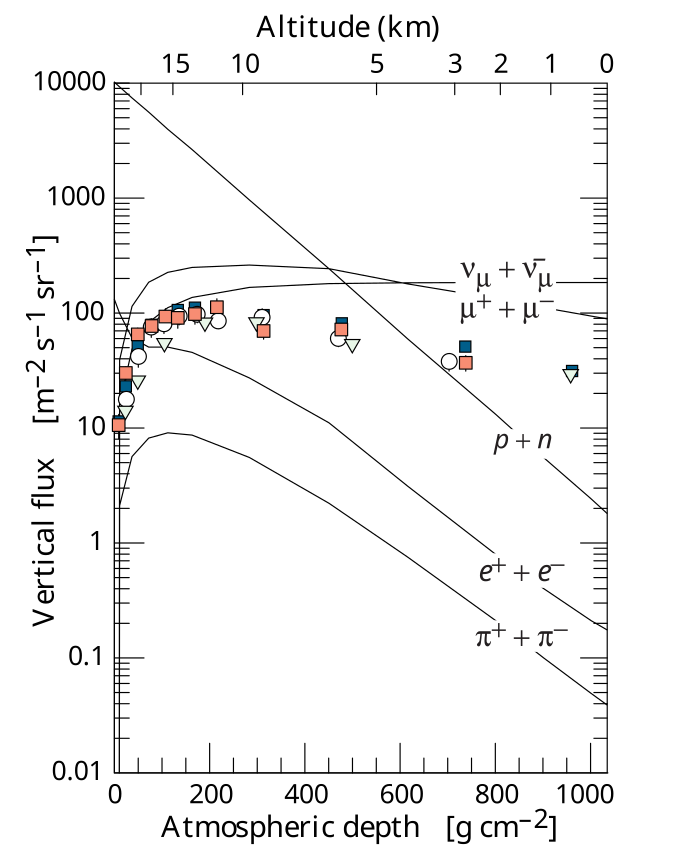
\includegraphics[width=0.95\linewidth]{../Imagenes/Cinderella.png}
		\captionof{figure}{Flujos verticales de rayos cósmicos en funcion de la altura \cite{EIDELMAN20041}.}
		\label{Fig:01}
	\end{center}
\end{minipage}

Entonces, ¿Cuáles son nuestros objetivos? Pues caracterizar la radiación cósmica incidente lo cual haremos diferenciando la \textit{componente dura} (partículas pesadas cargadas) como muones y la \textit{componente blanda} (partículas ligeras cargadas) como electrones/positrones, ver cuál es el ángulo de incidencia principal de los rayos cósmicos y ver cuál es la estadística de la radiación. Sin embargo previo a esto tendremos que hacer un estudio exaustivo de cómo realizamos las mediciones y cómo son nuestros detectores.

\section{Montaje experimental}

En el laboratorio constaremos de dos detectores plásticos de centelleo que denotaremos por ``1'' y ``2'' con fotomultiplicadores acoplados exactamente iguales colocados en paralelo tratando de superponer al máximo la superficie de entrada de la radiación y con las superficies lo más cercanas posibles (a menos que se indique lo contrario). La normal a la superficie de entrada de los detectores será normal a la normal del suelo en todas las medidas (a menos que se indique lo contrario).

Los detectores de centelleo se basan en la fluorescencia, que es el fenómeno por el cual una partícula excita los electrones del material quedando durante un pequeño periodo de tiempo en niveles superiores, de tal modo que cuando caen emiten fotones en el visible \cite{Knoll:1300754}. Cabe destacar que la energía emitida en forma de luz y la energía depositada por la partícula incidente no es estrictamente lineal (fórmula de Birk) \cite{Knoll:1300754}. Así pues los detectores de centelleo son sensibles a la energía del a partícula incidente. de tal modo que actúan como un primer discriminador: si no es capaz de excitar al electrón a una capa superior no se emite fotón de luz visible y por tanto no se detecta la partícula, además que es capaz de dar una respuesta muy corta (en nuestro caso de entorno a unos pocos nanosegundos). Esta es una de las razones por las cuales usamos los


\begin{minipage}{0.49\linewidth}
	\begingroup
	\setlength{\parskip}{2.2mm} % Cambia el espacio entre párrafos
	centelleadores, ya que nos sirven como un primer discriminador de radiación incidente, ya que nosotros buscamos principalmente muones y electrones cósmicos que tienen un rango de energía en la superficie de la tierra alto (de entorno unos GeV), tal y como se puede ver en el espectro \ref{Fig:02}.

	Sin embargo una de las razones es que nos dan una respuesta muy rápida de unos pocos nanosegundos. Esto nos permite tener una mejor resolución de las partículas incidentes en el material, ya que se minimized el tiempo de superposición entre dos rayos incidentes, de tal modo que más partículas pueden ser diferenciadas. De hecho esta rapidez también hace que perdamos eficiencia, al menos en comparación con otros centelleadores inorgánicos \cite{ElthonHo}.
	\endgroup
\end{minipage}
\hfill
\begin{minipage}{0.49\linewidth}
	\begin{center}
		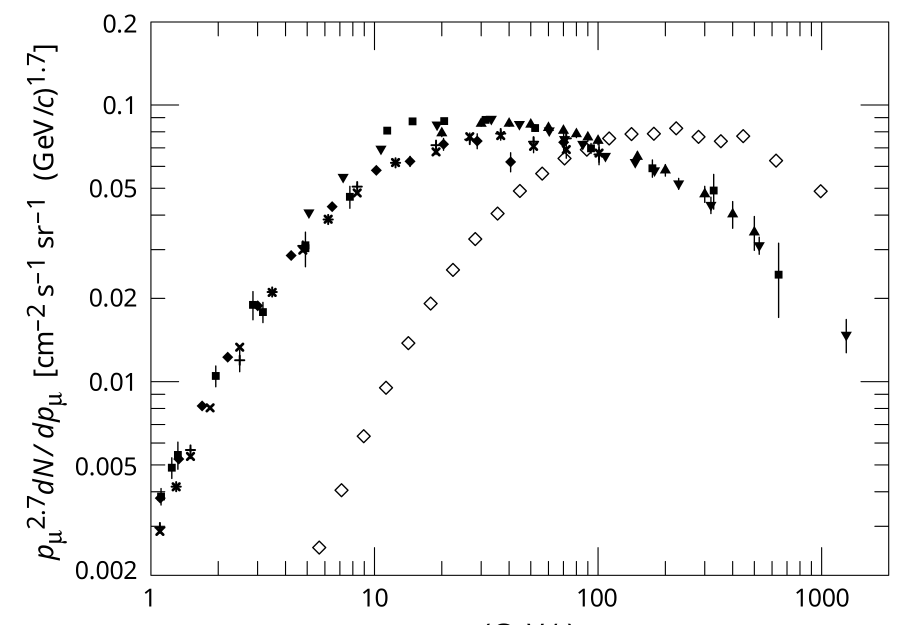
\includegraphics[width=0.95\linewidth]{../Imagenes/espectro.png}
		\captionof{figure}{Espectro de la energía muónica al nivel del mar a dos ángulos diferentes \cite{EIDELMAN20041}.}
		\label{Fig:02}
	\end{center}
\end{minipage}


A pesar de sus ventajas, por si mismo el centelleador no es capaz de producir suficientes fotones (quizás produce uno o dos) como para producir luz y mucho menos una señal medible en unidades ``macroscópicas'', por lo que es necesario que tengamos al final del mismo (en la dirección de los fotones) dos fotomultiplicadores. Su función prinicipal es aumentar el número de fotones gracias a una diferencia de potencial que llamaremos \textit{alto voltaje} o \textit{ganancia} que nos dará el módulo NIM CAEN de alto voltaje. Cuanta más alto sea este voltaje, se generarán más fotones habrá en la señal final. Esto sin embargo es un problema, ya que a partir de cierto voltaje se producirá un fenómeno de avalancha por el cual los fotones tendrán tanta energía enerǵia que podrán crear pares de electrón-positrón desvirtuando totalmente la medida,de tal modo que se pierda la proporcionalidad entre energía depositida y fotones emitidos. Este fenómeno se estudiará precisamente en el apartado \ref{Subsec:zona_trabajo}.

Tras esto lo que se hará es enviar la señal eléctrica producida por los fotones a través de un cable de unos 50-100cm de largo hacia un módulo NIM de umbral, que lo que hará es convertir la señal analógica en una señal lógica con una altura siempre que esta supere un valor regulado por el \textit{voltaje umbral} que podremos controlar en el laboratorio, y que también estudiaremos en \ref{Subsec:zona_trabajo}. Si la señal recibida es superior a la dictada por el umbral, se enviará al modulo de contaje y coincidencias, de tal modo que aumentará en una unidad el número de cuentas asociado al detector en cuestión.

Luego este módulo de contaje mostrará en una pantalla el número de cuentas que lleva tanto el detector 1 como el 2, y también enseñará el número de cuentas ``en coincidencia'', que son las realmente importantes. Las cuentas en coincidencia se definen como aquellas señales que provenientes de dos detectores diferentes llegan al modulo de contaje en un intervalo de tiempo inferior a la \textit{ventana de coincidencias}, de tal modo que si sucede las ``cuentas en coincidencia'' aumentará su valor en 1. ¿Por qué son las realmente importantes? Porque las cuentas en coincidencia son las que realmente miden los rayos cósmicos, ya que estos al tener tanta energía son capaces de depositar la energía en el detector 1 y 2 en una diferencia de tiempo de nanosegundos (son partículas  prácticamente lumínicas), de tal modo que la distancia entre una señal y otra al llegar al módulo de contaje será muy pequeña. En pocas palabras, todos los rayos cósmicos incidentes serán medibles a través de cuentas en coincidencia, mientras que otras partículas incidentes no serán medibles a traves de estas cuentas. Consecuentemente reduciremos el ruido ambiental y el ruido del detector/fotomultiplicador individual de cada detector.

Por tanto caracterizar nuestro detector significa analizar el comportamiento del número de cuentas en coincidencia variando los altos voltajes $V_1,V_2$, los voltajes umbral $U_1,U_2$ y conocer con precisión el valor de la ventana de coincidencias $\tau_{12}$, siendo esta una parte fundamental de esta memoria, particularmente porque de esta caracterización dependerá todo el análisis de los rayos cósmicos.


\section{Incertidumbre en las medidas}

\subsection{Incertidumbre de observables e incertidumbre de la tasa}

Una de las partes de mayor importancia en la práctica es el análisis de las incertidumbres, ya que como en todo experimento serán vitales para decidir si dos medidas son estadísticamente compatibles o son mutuamente descartables. Sin embargo su análisis no es trivial y mucho menos sencillo. Por eso dedicamos una sección entera a tratar las incertidumbres de cada medida que vamos a realizar: posibles fuentes, análisis sobre su tipo (A o B, \cite{GUM1995}). En el caso de dudas nos acogeremos a la sección 4.3.7 \cite{GUM1995}: <<In the absence of any knowledge about the possible values of an input quantity $X_i$ other than that they lie in an interval of width $2a$, and assuming that the values are equally probable, the rectangular distribution should be used>>. En todas las medidas, dado que no hemos hecho estadística de ninguna de ellas, la incertidumbre asiganda será de tipo B. \\

\begin{itemize}
	\begin{minipage}{0.65\linewidth}
		\item \textbf{Alto voltaje} ($V_1,V_2$): como hemos dicho hemos usado varios modulos NIM CAEN modelo 472 de alto voltaje tal y como mostramos en la imagen \ref{Fig:NIM}. Consultando el manual dado por el fabricante \cite{CAEN_N472} podemos ver que la incertidumbre asignada a las medidas para una lectura entre el 10\% y el 90\% del rango completo (siendo el máximo $6$kV), el error máximo es 1\% del valor leído. Como nostros daremos una ganancia de entorno a 1.5 a 2 kV, estamos dentro de ese rango. Así pues el valor de incertidumbre asignable a cada medida $V$, como máximo será:

		\begin{equation}
			u^{\max}_1(V) =\% 1 \ \unit{V}
		\end{equation}
		Sin embargo nosotros interpretamos que el fabricante nos da un intervalo de confianza con todos los valores dentro igual de probables, lo que se corresponde a una distribución rectangular \cite{GUM1995}. Eso nos lleva a:

		\begin{equation}
			u_1(V) = \frac{V}{\sqrt{3} \cdot 100} \ \unit{V}
		\end{equation}donde
		donde los cálculos están incluidos (sección 4.3.7 \cite{GUM1995}). Dado que para medir el valor hemos usado unos voltímetros, también tendremos que tener en cuenta la incertidumbre del voltímetro (independiente respecto al módulo). Como no conocemos al voltímetro usamos el  valor estándar asociada a uno de estos:
	\end{minipage}
	\hfill
	\begin{minipage}{0.3\linewidth}
		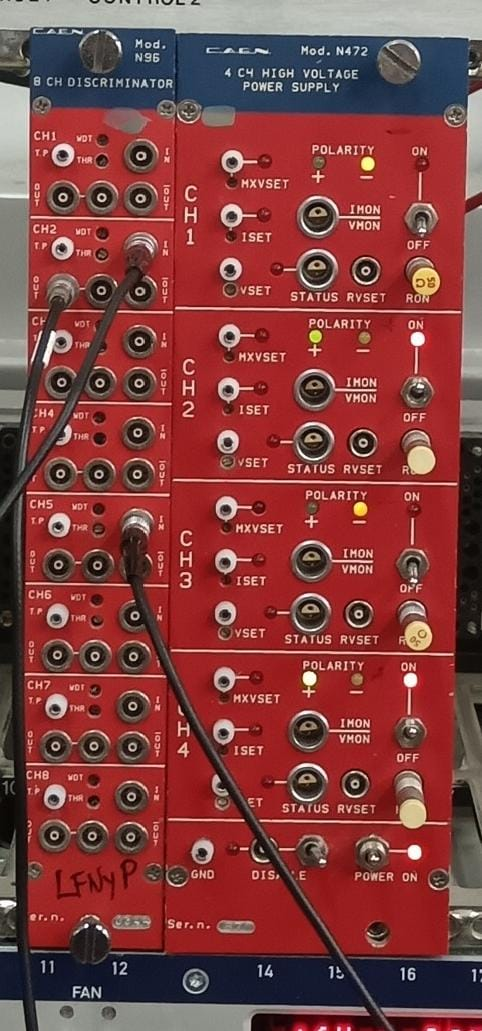
\includegraphics[width=0.94\linewidth]{../Imagenes/Modulo_NIm_Caen.jpeg}
		\captionof{figure}{Modulo NIM CAEN 472 (derecha), discriminador N96 (izquierda)}
		\label{Fig:NIM}
	\end{minipage}

	\begin{equation}
		u_2^{\max}(V) =  \% 1 + 2 \ \text{digit} \ \unit{V}  \rightarrow u_2(V) = \frac{1}{\sqrt{3}} \parentesis{  \% 1 + 2 \ \text{digit} } \label{Ec:03} \ \unit{V}
	\end{equation}
	dando como incertumbre total de la medida la combinación de ambas $u(V)=\sqrt{u_1(V)^2+u_2(V)^2}$.
	\item \textbf{Voltaje umbral} ($U_1,U_2$): para esto usamos un CAEN Mod. N96 – 8 Channel Discriminator (NIM) (véae imagen \ref{Fig:NIM}). Sin embargo no es aparece la información de la precisión o incertidumbre asociada a cada media en el manual \cite{CAEN_N96}, solo se nos dice que la precisión es de 1 mV, con lo que tendremos que conformarnos con asignar una incertidumbre a cada medida asociada con la distribución recctangular de anchura $2a$ siendo la anchura $a$ la precisión del aparato con la que la medimos, esto es, $a=0.001$ mV. Además incluiremos la precisión del polímetro igual que antes (ecuacion \ref{Ec:03} en mV), tal que
	      \begin{equation}
		      u_1 (U) = \frac{0.001}{\sqrt{3}} \ \unit{mV} \tquad u(U)=\sqrt{u_1(U)^2+u_2(U)^2} \ \unit{mV}
	      \end{equation}
	\item \textbf{Grosor de las placas} ($x$): el grosor de las placas las medimos con un calibrador analógico de precisión $0.05$ mm. Al igual que antes, solo sabemos el rango $2a$  en el que caen, asignadole una distribución uniforme tenemos:
	      \begin{equation}
		      u (x)  = \frac{0.05}{2\sqrt3} \ \unit{mm} \simeq 0.014 \ \unit{mm}
	      \end{equation}
	\item \textbf{Distancias entre detectores} ($d$): la distancia entre detectores las medimos a partir de un metro con una precisión de 1 mm. La fuente de incertidumbre con el metro no solo viene dada por su precisión, si no por su poca capacidad para mantenerse recto, añadiendo distancia ficticia debido a la posible curvatura del mismo. Le asignamos pues un valor $u_{1}=2$mm a la incertidumbre proveniente de este proceso. Además tendremos en cuenta la incertidumrbe dada por la precisión del aparato (distribución uniforme de anchura $1$ mm):
	      \begin{equation}
		      u_2 (d)  = \frac{1}{2\sqrt3} \ \unit{mm} \simeq 0.28 \ \unit{mm}
	      \end{equation}
	tal que $u(d)=\sqrt{u_1(d)^2+u_2(d)^2}=2.0$ mm.

	\item \textbf{Tamaños del detector} ($l$): ciertos tamaños como el grosor del detector los medimos con una regla de precisión 1mm. A diferencia de la distancia entre detectoroes, no tenemos ninguna razón para añadir más fuentes que incertidumbre que la precisión del aparato. Así pues: 
	\begin{equation}
		u (l)  = \frac{1}{2\sqrt3} \ \unit{mm} \simeq 0.28 \ \unit{mm}
	\end{equation}
	\item \textbf{Ángulos} ($\theta$): los ángulos los medimos con un transpondedor de ángulos de plástico de preqcisión $1^{\circ}$. No consideramos que haya otra fuente de incertidumbre, al menos en cuanto a la medición. Veamos entonces que:
	      \begin{equation}
		      u (\theta)  = \frac{1}{2\sqrt3} \ \unit{^\circ} \simeq 0.28 \ \unit{\unit{^\circ}}
	      \end{equation}
	\textcolor{blue}{En realidad la medida del ángulo sabemos que no es todo lo precisa que se indica aquí, pese a que no podamos añadir de manera explícita ningún factor de incertidumbre tipo B. Entonces lo que decidimos hacer es multplicar la incertidumbre aquí reflejada por un factor de cobertura $k=3$, correspondiente a un nivel de confianza aproximado del 99,7\%}.
	\item \textbf{Medidas de tiempo} ($t$): las medidas de tiempo son las más difíciles de analizar, ya que la precisión del aparato de medida (cronómetro de nuestros teléfonos móviles) es ridiculamente pequeña respecto al error asociado al proceso de toma de medidas.

	Para tomar una medida del número de cuentas y el tiempo lo que hacíamos era avisarnos mediante gestos verbales o visuales cuando uno apagaba la máquina del contaje para que el compañero inmediatamente parara el cronómetro. En general el proceso era advertido previamente, realizando comentarios del tipo, <<En 3, 2, 1...¡Ya!>>, de tal modo que minimizáramos el posible error, Nostros consideramos que como máximo nos podemos llegar a desviar entorno a $\Delta t=0.3$ s. Considerando que la mayor parte de las veces habrá una medida de tiempo inferior a esta, podemos consdierar que sigue una distribución triangular, de tal modo que:

	      \begin{equation}
		      u(t) = \frac{0.3}{\sqrt{6}} \approx 0.12
	      \end{equation}
	asociada a cada medida. En general esta media será despreciable frente a $\sqrt{N}$ que tendremos en cada medida de cuentas, aunque no por ello la descartaremos. Esta sería la incertidumbre de tipo B si la eligieramos hacer basado en estimaciones arbitrarias. La incertidumbre de tipo A la hacemos basado en el siguiente experimento. 

	Se han tomado dos conjuntos de datos: $x_1$, los tiempos reales medidos con cronómetro digital, y $x_2$, los tiempos anotados manualmente por un observador. A partir de ellos se construye la diferencia
	\[
	\Delta t = x_1 - x_2
	\]
	lo que nos permite estudiar el sesgo sistemático y la precisión del método manual. La gráfica: 

	\begin{figure}[h!] \centering
		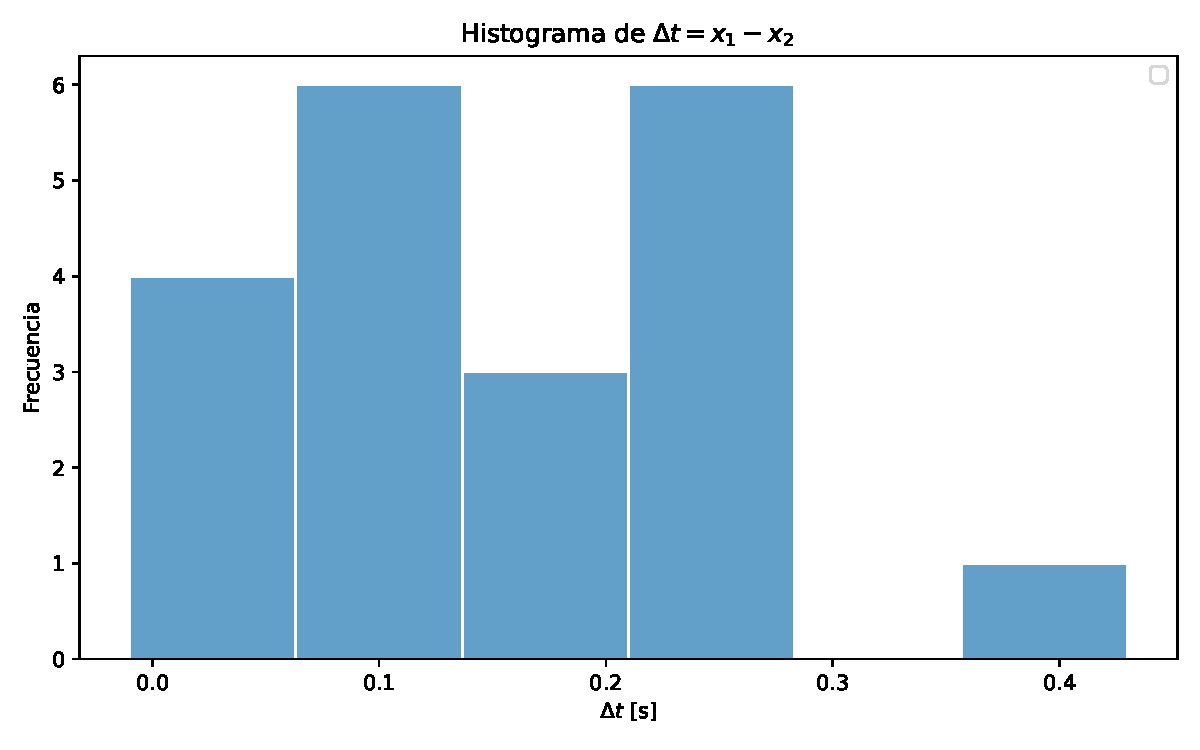
\includegraphics[width=0.6\linewidth]{../Tiempo.pdf}
	\end{figure}
	
	A partir de los 20 pares de datos obtenidos, calculamos los parámetors características de esta distribución.
	
	\begin{itemize}
		\item La media de las diferencias:
		\[
		\mu = \langle \Delta t \rangle = -0.152\ \text{s}
		\]
		Este valor indica que, en promedio, el observador tiende a anotar los tiempos con un retraso de aproximadamente 0.15 segundos respecto al valor real.
	
		\item La desviación típica:
		\[
		\sigma = \sqrt{ \frac{1}{N-1} \sum_{i=1}^{N} (\Delta t_i - \mu)^2 } = 0.111\ \text{s}
		\]
		que representa la variabilidad típica entre el valor real y el anotado manualmente. Este valor puede interpretarse como la incertidumbre tipo A asociada a cada medida individual de tiempo manual.
	
		\item La desviación estándar de la media:
		\[
		\sigma_{\mu} = \frac{\sigma}{\sqrt{N}} = 0.025\ \text{s}
		\]
		que cuantifica la incertidumbre en la estimación de $\mu$ como sesgo sistemático del procedimiento manual.
	\end{itemize}
	Podemos concluir entonces que, al menos estadísticamente, la incertidmbre asignada debiera ser $u(t)=0.11$.
	Este valor no es arbitrario, sino que refleja cuantitativamente la precisión experimental real del método empleado. La incertidumbre tipo A, basada en datos repetidos, garantiza que los errores aleatorios del procedimiento de medida estén correctamente evaluados y permite una trazabilidad estadística adecuada del experimento. Dado que hemos usado $0.12$ que no dista de este valor, y nos llevaría bastante tiempo cambiar todos los datos, decidmos mantener el uso de este 0.12, por comodidad. Una posterior revisión, con más tiempo podría incluir este factor. 
	
	

	\item \textbf{Cuentas:} este es el más importante de los observables. A un valor de cuentas $N$ le asignaremos una incertidumbre de $u(N)=\sqrt{N}$ ya que seguirá la distribución de Poisson, tal y como veremos en el apartado \ref{Sec:estadistica}. El error relativo es de $u(N)/N=1/\sqrt{N}$, y siempre tratamos de mantener que sea inferior al 5\%, lo que requiere un número de cuentas de entorno a $N=400$.
\end{itemize}
Estas son todas las medidas que realicemos. Las otros valores presentados a lo largo de la práctica será productos o funciones de estos A continuación vamos a presentar los como es la \textbf{tasa} $n=N/t$. La tasa que es un valor proveniente de dos observables con incertidumbre tendrá una incertidumbre asociada dada por la fórmula de propagación de incertidumbres (véase manual \cite{Estadistica}), tal que

\begin{equation}
	u(n) = \sqrt{\parentesis{\frac{u(N)}{t}}^2 + \parentesis{\frac{u(t)N}{t^2}}^2}
\end{equation}
el otro funcional que vamos a usar es la ventana de coincidencias $\tau$, pero como su fórmula necesita un poco de contexto lo comentaremos en su respectivo apartado \ref{Subsec:ventana_temporal}.

\subsection{Test $\chi^2$} \label{Subsec:chi_cuadrado}

El \textbf{test chi cuadrado} es una herramienta estadística que nos sirve para descartar o aceptar hipótesis realizadas sobre los datos con cierto nivel de confianza. El test de chi cuadrado se puede usar tanto para descartar o aceptar distribuciones de probabilidad, medias o bondades de ajuste (sección 3.3, \cite{Estadistica}). 

\textcolor{blue}{Nosotros vamos a usarlo en particular para descartar o aceptar las hipótesis de bondades de ajuste} (es decir, de regresiones lineales, exponenciales...). Consideremos entonces que hemos ajustado un conjunto de datos $\{  (x_i,y_i)\}_{i=1}^n$ a una ecuación $y=f(x)$. Definimos el valor $\chi^2$ de nuestro ajuste como:

\begin{equation}
	\chi^2 = \sum_{i=1}^n \frac{\ccorchetes{y_i-f(x_i)}^2}{s^2(y_i)}
\end{equation}
Sea $n-r$ el número de grados de libertad de nuestra distribución $\chi^2$ donde $r$ es el número de parámetros con los que hayamos ajutado $f(x)$. Entonces, para un nivel de confianza $\alpha$ rechazamos la hipótesis (nuestros datos se comportan tal que $y=f(x_i)$) si $\chi^2_{\alpha,n-r} \leq \chi^2$ donde $\chi^2_{\alpha,n-r}$ es el valor del percetil de la distribución con dichos grados de libertad y un nivel de confianza $\alpha$, \cite{Estadistica}. Cabe destacar que esto asume que $y_i$ se distribuye de modo gaussiano en torno a su valor medio $\bar{y}_i$. Nosotros para todos los ajustes y su $\chi^2$ usaremos C++ CERN ROOT \cite{Root}. \textcolor{blue}{En el caso del test aplicado a las distribuciones de probabilidad lo discutiremos en el apartado correspondiente.}


\section{Caracterización de los detectores}

En esta sección vamos a caracterizar los detectores, que tal y como hemos dicho, implica concoer el comportamiento de las cuentas en coincidencia respecto los valores de alto voltaje y de voltaje umbral, así como saber cual es el valor de la ventana de coincidencias. Primero determinaremos la zona de trabajo.



\subsection{Determinación de la ventana temporal} \label{Subsec:ventana_temporal}

Además de los eventos en coincidencia, cada detector producirá un número de pulsos que no pertenecerán a emisiones en coincidencia. Estos eventos no coincidentes, debido a su naturaleza aleatoria, es posible que se generen en un rango de tiempo suficientemente pequeño como para que sean detectadas como coincidencias. Nuestro objetivo claramente está en minimizar esta coincidencia aleatoria y maximiar las coincidencias reales, por ejemplo aumentando el voltaje umbral, o disminuyendo la actividad de la fuente Cap. 18 Knoll \cite{Knoll:1300754}. \textcolor{blue}{Dado que esto último es imposible, los centraremos en lo primero}. Cabe destacar que el cambio en la geometría afecta de igual manera a tanto al as accidentales como a las reales, por lo que podemos usar los valores obtenidos aquí en toda la práctica.

Entonces, ¿Cuál es el fin último de este apartado? Obtener la ventana de coincidencias, ¿Por qué? Porque es necesario conocerla para poder obtener la tasa de coincidencias accidentales en cada medida, que conociendo la tasa de coincidencias medidas nos dará un valor de la tasa de coindiencias reales, que usaremos en el resto de la práctica.

Así pues, sea $n_{acc}$ es la tasa de coincidencias accidentales, $n_1$ y $n_2$ son las tasas de cada uno de los detectores individuales, entonces $\tau$ que es la ventana de coincidencias viene dada por:
\begin{equation}
	n_{acc} = 2 \tau  n_1 n_2
\end{equation}
ecuacion 17.28 \cite{Knoll:1300754}. Despejando para obtener $\tau$:

\begin{equation}
	\tau = \frac{n_{acc}}{2 n_1 n_2}
\end{equation}
así pues, tenemos que la incertidumbre total de la ventana de coincidencias.

\begin{equation}
	u(\tau) = \sqrt{\parentesis{\frac{u(n_{acc})}{2n_1n_2}}^2+\parentesis{\frac{n_{acc}}{2n_1^2n_2} u(n_1)}^2+\parentesis{\frac{n_{acc}}{2n_1n_2^2} u(n_2)}^2}
\end{equation}
Sin embargo nosotros no podemos medir $n_{acc}$, nosotros medimos $n_{12}$. Para asegurarnos que todas las medidas de $n_{12}$ son accidentales lo que hicimos fue cruzar los detectores de tal modo que $N_{12}\approx N_{acc}$, siendo los datos obtenidos representados en la \cref{Tab:ventana_01}.

\hspace*{-1.0cm} \begin{center}
\begin{table}[H]
\caption{Ventana de coincidencias}
\label{Tab:ventana_01}
\begin{tabular}{cccccccccccccccccccccc}
\toprule
$N_1$ & $N_2$ & $N_{12}$ & $t$ (s) & $n_1$ (s$^{-1}$) & $n_2$ (s$^{-1}$) & $n_{12}$ (s$^{-1}$) & $\tau$ ($\mu$s) \\
\midrule
\num{45323.0000000000(212.8919913947)} & \num{10854.0000000000(104.1825321251)} & \num{154.0000000000(12.4096736460)} & \num{94.2100000000(0.3000000000)} & \num{481.0848105297(2.7300916193)} & \num{115.2106995011(1.1651224443)} & \num{1.6346460036(0.1318263382)} & \num{14.7461709041(1.2014395137)} \\
\num{84902.0000000000(291.3794776576)} & \num{21458.0000000000(146.4854941624)} & \num{268.0000000000(16.3707055437)} & \num{184.6800000000(0.3000000000)} & \num{459.7249296080(1.7455667243)} & \num{116.1901667750(0.8153325141)} & \num{1.4511587611(0.0886749683)} & \num{13.5836818887(0.8370943900)} \\
\num{48572.0000000000(220.3905624114)} & \num{21615.0000000000(147.0204067468)} & \num{103.0000000000(10.1488915651)} & \num{98.1000000000(0.3000000000)} & \num{495.1274209990(2.7092109749)} & \num{220.3363914373(1.6431861470)} & \num{1.0499490316(0.1035043668)} & \num{4.8121040597(0.4764626054)} \\
\num{43165.0000000000(207.7618829333)} & \num{16088.0000000000(126.8384799657)} & \num{181.0000000000(13.4536240471)} & \num{101.7400000000(0.3000000000)} & \num{424.2677413014(2.3948291109)} & \num{158.1285630037(1.3310341506)} & \num{1.7790446236(0.1323393577)} & \num{13.2588699141(0.9954110424)} \\
\bottomrule
\end{tabular}
\end{table}
\end{center}


Cabe destacar que el último valor lo medimos con dos voltajes umbrales diferentes $U_1,U_2=-0.0750(29)$ para así aumentar el número de accidentales. En el laboratorio también medimos una medida extra aquí no representada, ya que fueron mal tomados los datos. Aplicando ahora la media ponderada y la incertidumbre de la media ponderada podemos obtener un valor $\tau$: 

\begin{equation}
	\tau = 13.74 \ \unit{\mu s^{-1}} \qquad  u(\tau) = 0.57  \ \unit{\mu s^{-1}}
\end{equation}
Como podemos ver la incertidumbre obtenida por la media ponderada parece que no refleja del todo bien la distribución real de nuestros datos. Este fenómeno llamado \textbf{sobredispersión e infradispersión} y ocurre cuando usamos medias ponderadas. 
Una manera estándar de diagnosticar la sobredispersión es mediante el cálculo del estadístico de \(\chi^2\), definido como:

\begin{equation}
\chi^2 = \sum_{i=1}^{n} \frac{(x_i - \bar{x})^2}{\sigma_i^2}
\end{equation}
donde \(x_i\) son las mediciones individuales, \(\sigma_i\) sus respectivas incertidumbres, y \(\bar{x}\) la media (ponderada). Si el valor reducido \(\chi^2/\text{ndf}\) (con \(\text{ndf} = n - 1\)) es mucho mayor que uno, se considera que hay sobredispersión. En tal caso, es habitual corregir la incertidumbre de la media multiplicándola por \(\sqrt{\chi^2/\text{ndf}}\), para reflejar más fielmente la variabilidad observada. Sin embargo en nuestro caso los datos están infradispersados $\chi^2$/ndf = 0.4849 con ndf=2, y en estos casos no se suelen aplicar correcciones. 
 
Este valor es efectivamente un valor que podríamos esperar. Una ventana de coincidencias mayor haría que aumentará la tasa de coincidencias accidentales sin aumentar las verdaderas, mientras que una menor podría hacer que una tasa de coincidencias real no se midiera. ¿Como es esto último posible, si hemos dicho al principio que entre una y otra medida proveniente de un rayo cósmico hay entorno a unos pocos nanosegundos? Si, esto último es cierto, pero  hay más procesos aparte de este: la señal tiene que propagarse por el centelleador, ser multiplicada por el fotomultiplicador, y tiene que enviarse a través de cables con una posible diferencia calidad y tamaño. Una pequeña diferencia de varios centímetros en el cable ya produciría esta diferencia. Veamos numéricamente esto.

Por ejemplo, si uno de los cables que lleva la señal es unos \SI{0.5}{\meter} más largo que otro, y considerando que la señal viaja a una velocidad de aproximadamente, \( v = \SI{2e8}{\meter/\second} \), lo cual es cierto suponiendo cables coaxiales con velocidad de fase \(\sim 2/3\) de \(c\)), el retraso introducido es:

\[
\Delta t = \frac{\Delta x}{v} = \frac{0.5~\text{m}}{2 \times 10^8~\text{m/s}} = 0.25~\text{ns}
\]

A esto debemos sumar las dispersiones típicas del fotomultiplicador (\(\sim 5\)-\(10~\text{ns}\)) y la propagación interna en el centelleador (\(\sim 1\)-\(10~\text{ns}\)). El retraso total acumulado puede fácilmente situarse en el rango de:

\[
\Delta t_{\text{total}} \approx 30\text{ a }50~\text{ns}
\]

Considerando estas fluctuaciones no llegamos ni a un microsegundo de valor de la ventana. Entonces, ¿Cual puede ser la razón? El motivo tiene que ser el ancho temporal de la señal eléctrica, que estudiamos en los primeros compases de la práctica. Aunque el retardo físico entre la llegada de un mismo muón a dos detectores es del orden de los nanosegundos, el ancho temporal de la señal eléctrica generada por cada evento (principalmente determinado por la respuesta del PMT y del sistema de discriminación) puede extenderse hasta \SI{10}{\micro\second} o más. Para asegurar que los pulsos se solapen temporalmente dentro de la lógica de coincidencias, la ventana debe ser al menos tan ancha como estos pulsos. Aún así un estudio completo necesitaria más detalles y tiempo en este aspecto de la práctica.

Así pues, conocido $n_1$ y $n_2$ podemos calcular fácilmente la \textbf{tasa de coincidencias accidentales} $n_{acc}$ y obtener entonces la \textbf{tasa de coincidencias reales} $n_r$ como:

\begin{equation}
	n_{acc} = 2 \tau n_1 n_2 = 2\sqrt{(u({\tau})n_1n_2)^2 + (u(n_{1})\tau n_2)^2  (u(n_{2})\tau n_1)^2 }
\end{equation}
\begin{equation}
	n_r = n_{12} - n_{acc} \qquad u(n_r) = \sqrt{u(n_{12})^2 + u(n_{acc})^2}
\end{equation}

\subsection{Determinación de la zona de trabajo} \label{Subsec:zona_trabajo}

Es muy importante elegir bien los pares de valores $V_1,V_2,U_1$ y $U_2$. Si, por ejemplo, $V$ fuera demasiado grande, es probable que entraramos en una zona de avalancha del multiplicador perdiendo toda la información de las medidas. Por otro lado, si fuera muy pequeño, es probable que las medidas reales no fueran suficientemente amplificadas para que sean detectadas. Lo mismo ocurre con el valor umbral $U$, si es muy grande las medidas se reducirán hatsa un punto en el que no veamos nada, mientras que si es muy bajo detectaremos medidas espurias, que tienen los siguientes orígenes: 


\begin{itemize}
    \item \textbf{Ruido térmico y electrónico}: generado en los fotomultiplicadores o por la electrónica asociada. Aumenta con el voltaje de ganancia o con umbrales demasiado bajos.

    \item \textbf{Luz ambiental}: el centelleador es sensible a la luz visible, por lo que un aislamiento deficiente puede inducir falsas señales.

    \item \textbf{Radiación ambiental no cósmica}: como la radiactividad natural o fuentes externas que generan cuentas individuales que podrían coincidir aleatoriamente.

    \item \textbf{Desajustes de cableado o electrónica}: diferencias en la longitud de los cables o errores en el ajuste de la ventana temporal pueden inducir falsos positivos en las coincidencias.
	\item \textbf{Oscilaciones en la señal de la red} pueden producir estos desajustes.
    \item \textbf{Fotogeneración de portadores.} No es lo mismo que las detecciones de fotones ambientales. 
    \item \textbf{Extracción de electrones por voltaje no nulo.} Debido a fluctuaciones cuánticas. 
\end{itemize}
\textcolor{blue}{Un estudio más detallado requeriría la comprensión de cada uno de estos orígenes, correción y modelización. Para esto podríamos usar información acerca de las señales estudiadas en la primera parte de la práctica, o hacer un estudio más detallado de las coincidencias accidentales (ventana temporal) con otros montajes. }


Lo que queremos nosotros es precisamente estar en la región en la que ambos valores estén compensados: que todas las medidas de rayos cósmicos sean suficientemente amplificados y medidos, con el menor ruido. Esto que acabamos de contar de manera naif se conoce en la literatura por \textit{counting plateu}, región en la que el experimento tiene una sensitividad mínima al ruido/medidas espúreas Cap. 4 \cite{Knoll:1300754}. \textcolor{blue}{Existen varias maneras de detectar un plateu, pero el que nostros vamos a usar es estudiar la variación de $n_{acc}/n_r$, observando a partir de qué punto podemos considerar que comienzan a dominar fuertemente las coincidencias accidentales frente a las reales. El plateu estará en la región en la que dominen fuertemente las reales (idealmente $n_{acc}/n_r=0$).}


\subsubsection{Estudio de $U_1$}


En la tabla \ref{Tab:plateu_U} podemos ver las medidas tomadas, mientras que en la \cref{Fig:plateuU} vemos su representación gráfica.En el proceso de medida lo que hicimos fue coger un valor máximo  y el mínimo de $U_1$ basado en información dada por otros compañeros. Entonces decidimos coger tres de valores más en el medio, y vimos que efectivamente parecía que había un comportamiento esperado, con una una región plana y un salto exponencial en el rango de $U_1\approx 90$ mV. Los otros valores constantes fueron: $V_2=1.888$ V, $U_2=-0.101$ V y $V_1=1.899$ V.

La eleción del plateu no es trivial, y lo que nosotros decidimos fue coger un valor relativamente pequeño de $U_1\approx - 0.100$ V ya que  está en el plateu como los otros valores, y al ser un poco más laxo con el umbral consdieramos que tendríamos más cuentas. Lo que esta claro es que entre -0.100 y -0.050 es en la región donde las coincidencias accidentales comienzan a dominar, lo cual no nos intersa. 

\begin{figure}[h]
		\centering
		\caption{Cociente entre medidas accidentales y reales.}
		\label{Fig:plateuU}
		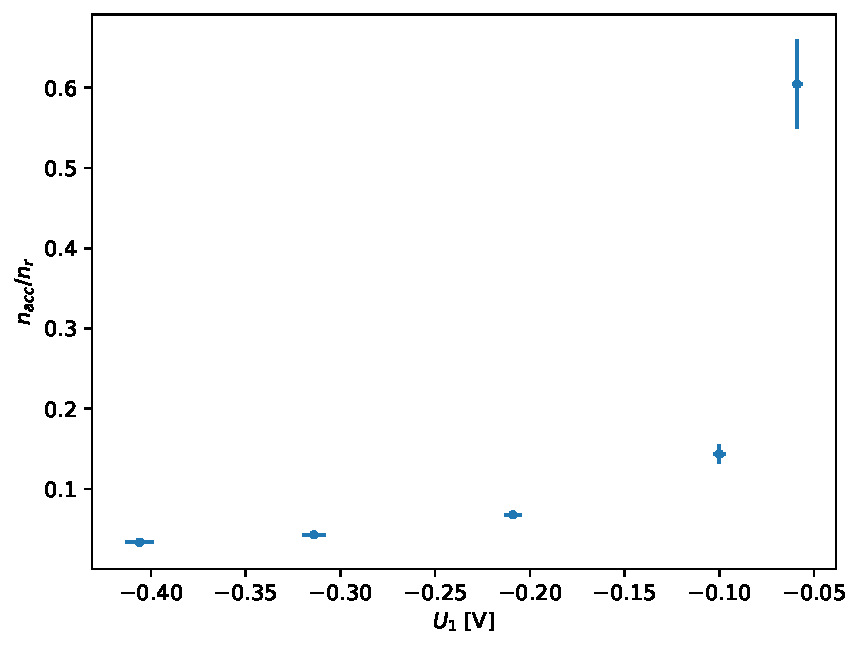
\includegraphics[width=0.6\linewidth]{../Graficas/GraficoU2.pdf}
\end{figure}

\begin{center}
\begin{table}[H]
\caption{Medidas fijando el voltaje umbral}
\label{Tab:plateu_U}
\begin{tabular}{cccccccccccccccccccccc}
\toprule
$U_1$ (V) & $N_1$ & $N_2$ & $N_{12}$ & $t$ (s) & $n_1$ (s$^{-1}$) & $n_2$ (s$^{-1}$) & $n_{12}$ (s$^{-1}$) \\
\midrule
\num{-0.0590000000(0.0100000000)} & \num{1822.0000000000(42.6848919408)} & \num{40815.0000000000(202.0272258880)} & \num{350.0000000000(18.7082869339)} & \num{15.5000000000(0.3000000000)} & \num{117.5483870968(3.5721119464)} & \num{2633.2258064516(52.6059323045)} & \num{22.5806451613(1.2836759428)} \\
\num{-0.1000000000(0.0100000000)} & \num{9944.0000000000(99.7196068985)} & \num{3040.0000000000(55.1361950084)} & \num{223.0000000000(14.9331845231)} & \num{29.7200000000(0.3000000000)} & \num{334.5895020188(4.7607781038)} & \num{102.2880215343(2.1231615365)} & \num{7.5033647376(0.5081389212)} \\
\num{-0.3140000000(0.0100000000)} & \num{3764.0000000000(61.3514466007)} & \num{6482.0000000000(80.5108688315)} & \num{318.0000000000(17.8325545001)} & \num{51.4500000000(0.3000000000)} & \num{73.1584062196(1.2664526335)} & \num{125.9863945578(1.7286913207)} & \num{6.1807580175(0.3484683485)} \\
\num{-0.2090000000(0.0100000000)} & \num{6250.0000000000(79.0569415042)} & \num{5667.0000000000(75.2794792756)} & \num{323.0000000000(17.9722007556)} & \num{47.5200000000(0.3000000000)} & \num{131.5235690236(1.8593526864)} & \num{119.2550505051(1.7539650572)} & \num{6.7971380471(0.3806294656)} \\
\num{-0.4060000000(0.0100000000)} & \num{8208.0000000000(90.5980132232)} & \num{3060.0000000000(55.3172667438)} & \num{320.0000000000(17.8885438200)} & \num{66.5100000000(0.3000000000)} & \num{123.4100135318(1.4715207894)} & \num{46.0081190798(0.8572127469)} & \num{4.8113065704(0.2698343347)} \\
\bottomrule
\end{tabular}
\end{table}
\end{center}


\begin{figure}[H]
	\centering
	\caption{Medidas accidentales, reales y totales frente $U_1$ \cite{Root}.}
	\label{Fig:plateuU2}
	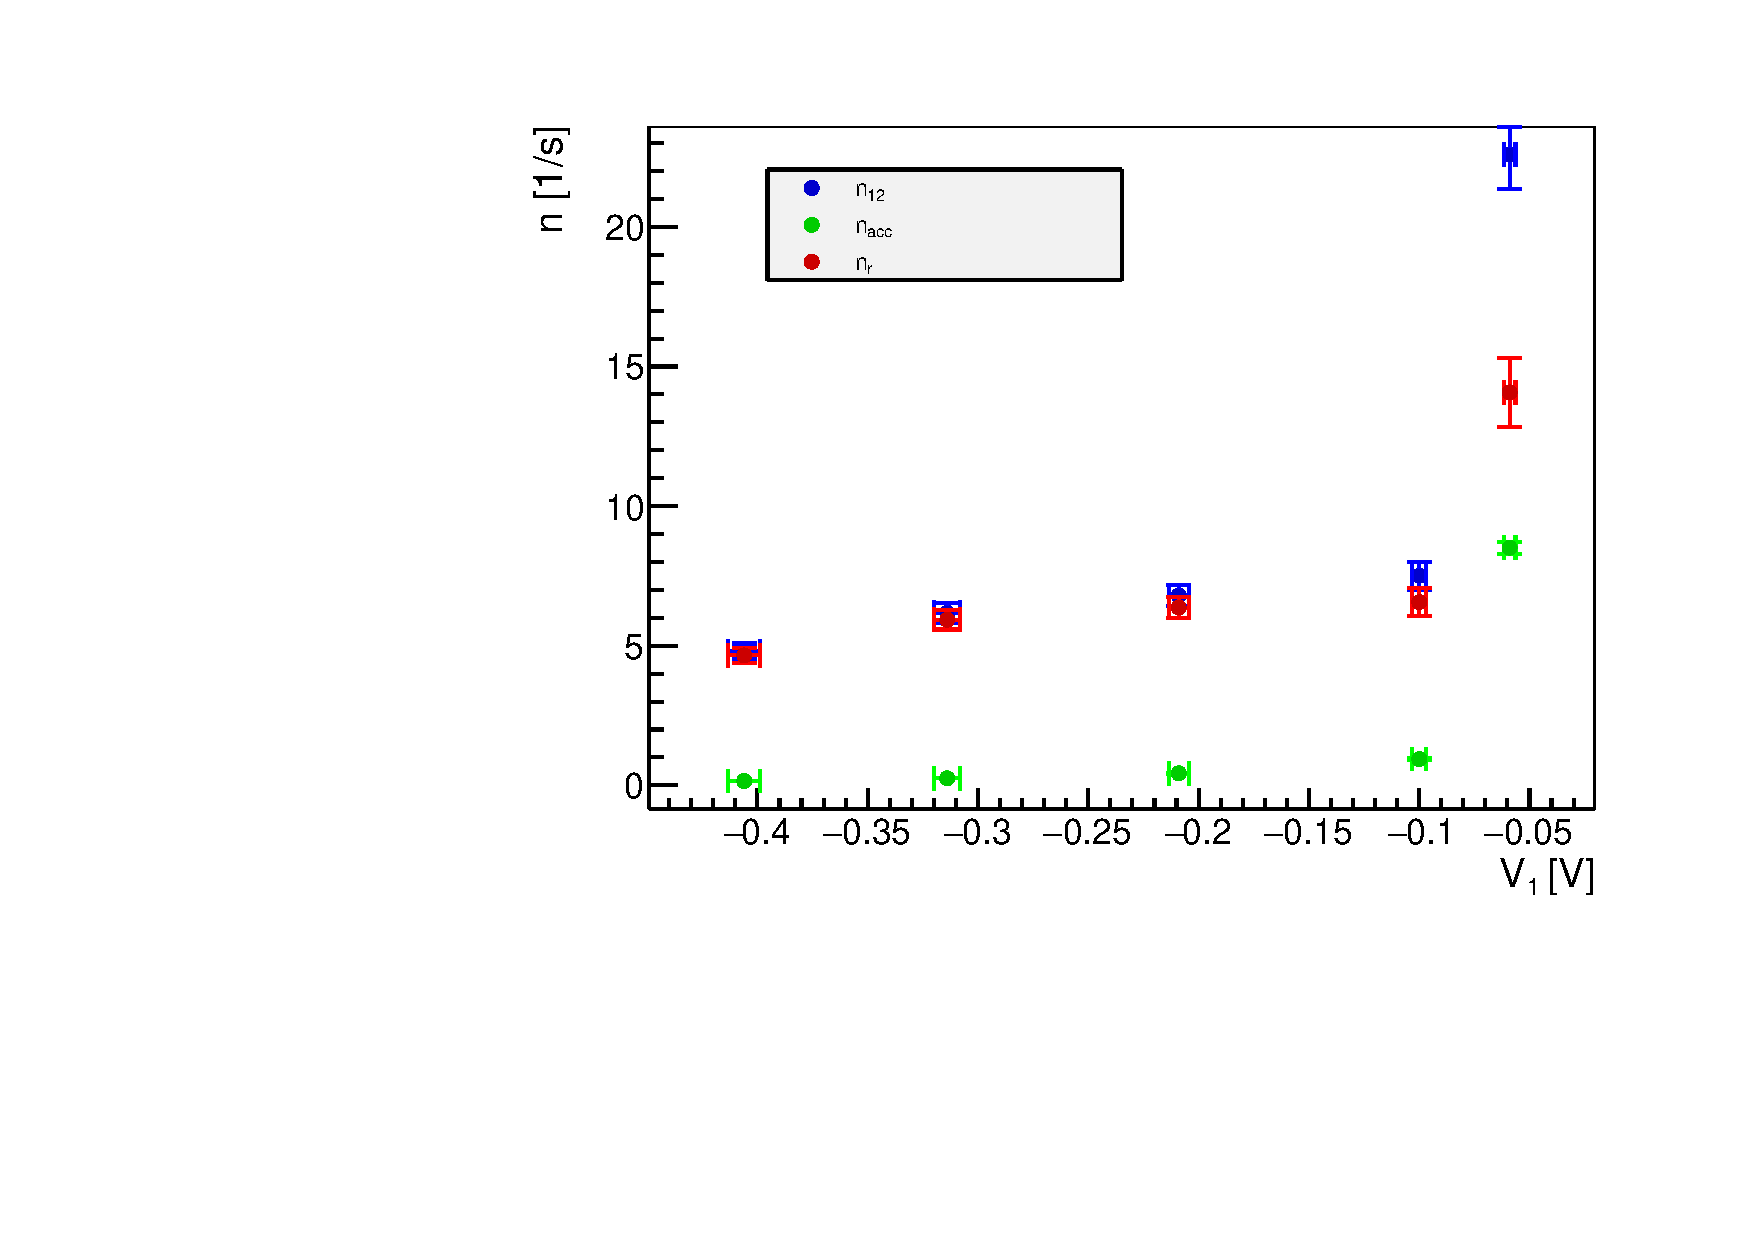
\includegraphics[width=0.6\linewidth]{../Graficas/GraficoU.pdf}
\end{figure}

\subsubsection{Estudio de $V_1$}

En la tabla \ref{Tab:plateu_V} podemos ver las medidas tomadas, mientras que en la \cref{Fig:plateuV} vemos su representación gráfica.En el proceso de medida lo que hicimos fue coger el valor máximo  y el mínimo de $V_1$ que nos dictaba la seguridad en el laborato y el aparato (respectivamente), con lo que comprobamos efectivamente que no había mucha distancia entre el $n_{12}$ de ambos. Entonces decidimos coger un par de valores en el medio y tras una rápida representación en Excel nos dimos cuenta de que no parecía comportarse como esperábamos, no hay una región particularmente plana. 

Nosotros decidimos fue coger un valor relativamente grande de $V_1\approx 1.910$ V ya que al tener más ganancia tendríamos más cuentas (tampoco podemos decir que estas medidas tienen más ruido que cualquier otra). Como podemos ver en la siguiente imagen \ref{Fig:plateuV} en general dominan las tasas de coincidencias reales, aunque a partir de 1.9 kV es cuando comienza a doinar de verdad, por lo que nuestra elección fue justo cortar en este punto con un 3 tasa accidental cada 20 reales, y aumentar el número de medidas

\begin{figure}[h!]
	\centering
	\caption{Cociente entre medidas accidentales y reales.}		\label{Fig:plateuV}
	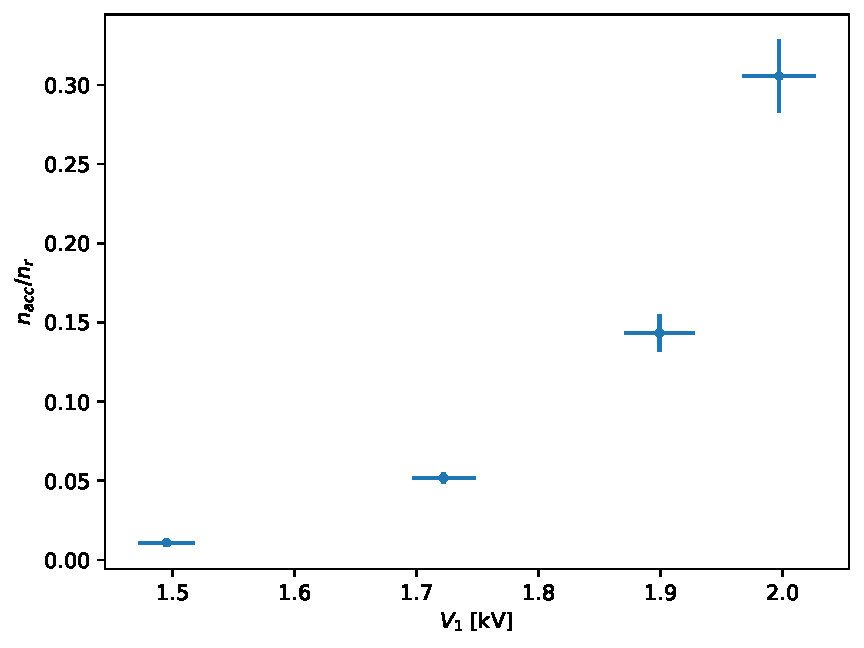
\includegraphics[width=0.6\linewidth]{../Graficas/GraficoV2.pdf}
\end{figure}

\begin{center}
\begin{table}[H]
\caption{Medidas fijando el voltaje de ganancia}
\label{Tab:plateu_V}
\begin{tabular}{cccccccccccccccccccccc}
\toprule
$V_1$ (V) & $N_1$ & $N_2$ & $N_{12}$ & $t$ (s) & $n_1$ (s$^{-1}$) & $n_2$ (s$^{-1}$) & $n_{12}$ (s$^{-1}$) \\
\midrule
\num{1.4950000000(0.0100000000)} & \num{1026.0000000000(32.0312347561)} & \num{7436.0000000000(86.2322445492)} & \num{300.0000000000(17.3205080757)} & \num{65.2900000000(0.3000000000)} & \num{15.7145045183(0.4958845879)} & \num{113.8918670547(1.4206560605)} & \num{4.5948843621(0.2661245915)} \\
\num{1.7220000000(0.0100000000)} & \num{4737.0000000000(68.8258672303)} & \num{5695.0000000000(75.4652237789)} & \num{308.0000000000(17.5499287748)} & \num{48.9200000000(0.3000000000)} & \num{96.8315617334(1.5270897701)} & \num{116.4145543745(1.6998107824)} & \num{6.2959934587(0.3608192229)} \\
\num{1.8990000000(0.0100000000)} & \num{9944.0000000000(99.7196068985)} & \num{3040.0000000000(55.1361950084)} & \num{223.0000000000(14.9331845231)} & \num{29.7200000000(0.3000000000)} & \num{334.5895020188(4.7607781038)} & \num{102.2880215343(2.1231615365)} & \num{7.5033647376(0.5081389212)} \\
\num{1.9970000000(0.0100000000)} & \num{24917.0000000000(157.8511957509)} & \num{3904.0000000000(62.4819974073)} & \num{338.0000000000(18.3847763109)} & \num{33.7900000000(0.3000000000)} & \num{737.4075170169(8.0427679934)} & \num{115.5371411660(2.1145914584)} & \num{10.0029594555(0.5512897016)} \\
\bottomrule
\end{tabular}
\end{table}
\end{center}


\begin{figure}[h!] \centering
	\caption{Medidas accidentales, reales y totales frente $V_1$ \cite{Root}.}	\label{Fig:plateuV2}
	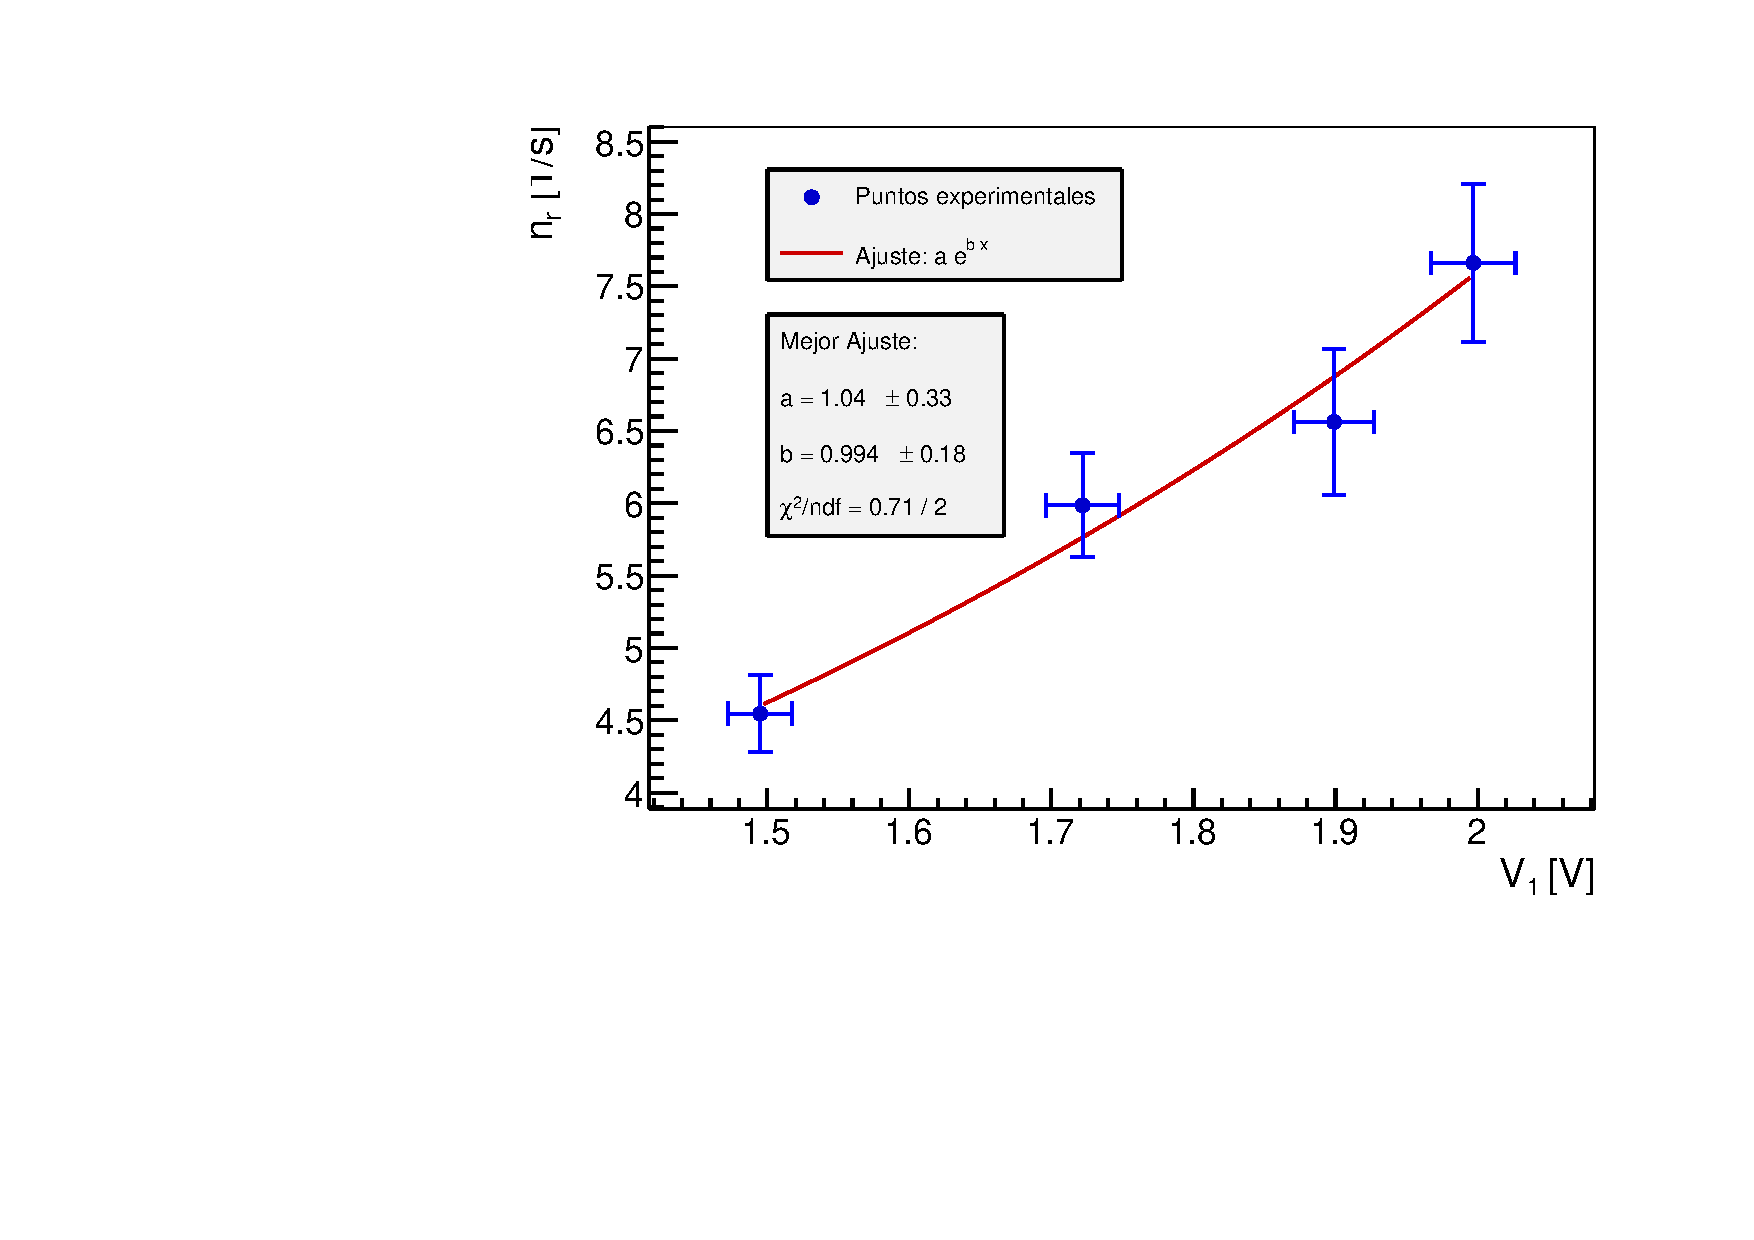
\includegraphics[width=0.6\linewidth]{../Graficas/GraficoV.pdf}
\end{figure}


\subsubsection{Elección de alto voltaje y umbral}

Finalmente elegimos los valores de $V_1,V_2=1.911(28)$ kV y $U_1=101(32)$ mV y $U_2=110(36)$ mV para el resto de valores. ¿Por qué? En primer lugar, consieramos que una valor de alto voltaje alto (sin pasarse de 1.95 kV) es conveniente ya que auemntará el número de cuentas y como hemos podido comprobar no está ``más en el plateu'' que cualqueir otro valor. Por otro lado, al auemntar los altos voltajes decidimos aumentar ligeramente los valores de $U_1$ y $U_2$ ya que podrá eliminar medidas espureas y aún estaría en el plateu. 



\section{Caracterización estadística de la radiación cósmica secundaria} \label{Sec:estadistica}

Tras caracterizar nuestro detector y su comportamiento, ahora ya podemos estudiar los rayos cósmicos secundarios. Tal y como se nos dice en el guión de la práctica \cite{P2}, en principio tanto la radiación cósmica como las coincidencias accdientales siguen una distribución de Poisson. ¿Cómo comprobamos, que, efectivamente, siguen una distribución de Poisson? Pues simplemente estudiando el número de cuentas que hay en diferentes intervalos de tiempo y luego representar el histograma de frecuencias, haciendo una bondad de ajuste a una poissoniana, para luego hacer una comprobación con el test de $\chi^2$. También incluiremos una gaussiana, por razones que serán comentadas posteriormente. Primero comentaremos un poco la adquisición de datos que realizamos, ya que es peculiar; luego realizaremos un análisis detallado sobre el test $\chi^2$ aplicado a este problema y sobre la distribucción de Poisson. Posteriormente comentaremos la tendencia a la distribución de gauss cuando el número de cuentas es elevado y finalmente analizaremos los resultados. 

\subsection{Análisis del vídeo: red neuronal}

El estudio aquí presente se realizo analizando una aproximadamente hora y veinte minutos de vídeo, lo cual, en cuentas con un intervalo de 1 segundo serían aproximadamente unos 5250 datos. Lógicamente nos parecía inviable tomar cada uno de estos a mano, parando el video cada segundo. Lo que hicimos fue con un programa de python (a través de los módulos \href{https://pypi.org/project/opencv-python/}{cv2} y \href{https://pypi.org/project/pytesseract/}{pytesseract}) que nos sacaba imágenes de los fotogramas que quisiéramos (así, podíamos ir desde 1 segundo a 0.1 segundos, si quisiéramos). Además no solo contabamos con obtener fotogramas, si no que podíamos cortar la imagen y seleccionar un cacho del video \cref{Fig:video} y trasformarlo en blanco y negro \cref{Fig:fotograma}, lo cual es óptimo para el reconocimiento por una red neuronal.

\begin{minipage}[t]{0.45\linewidth}
	\begin{center}
	\captionof{figure}{Fotograma aleatorio del video.}  
	\label{Fig:video}
	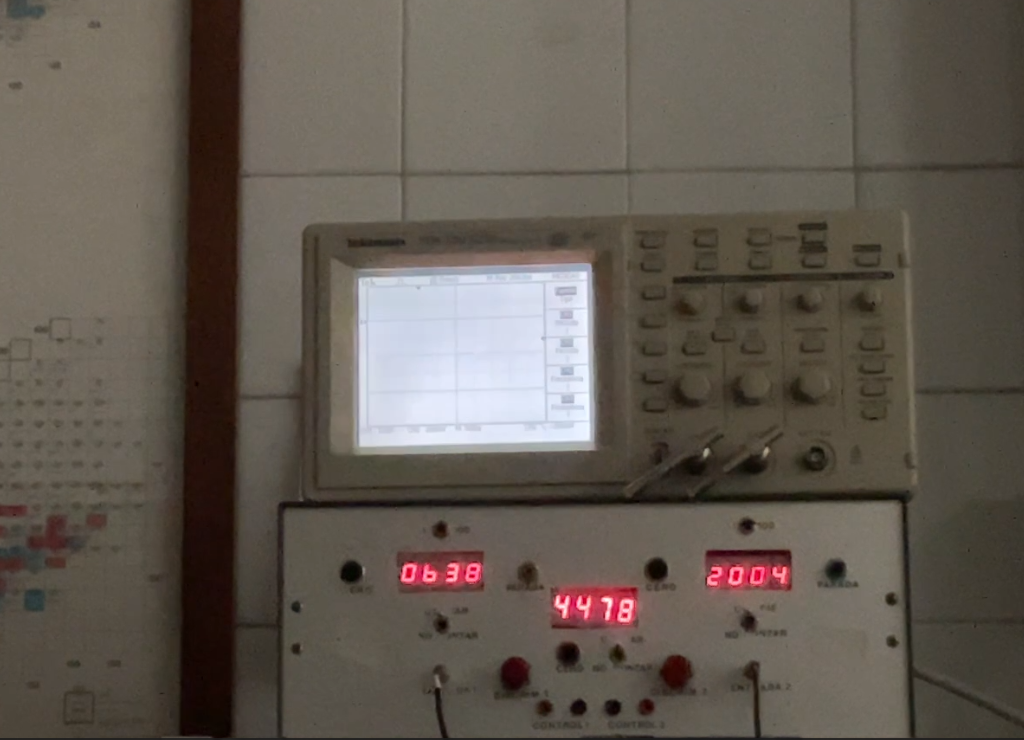
\includegraphics[width=0.75\linewidth]{../Imagenes/VideoOriginal.png}
	\end{center}
\end{minipage}	
\hfill
\begin{minipage}[t]{0.5\linewidth}
\begin{center}
	\captionof{figure}{Fotogramas individuales}  
	\label{Fig:fotograma}
	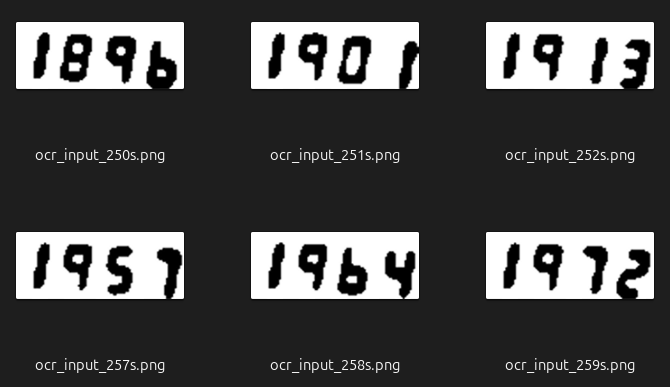
\includegraphics[width=0.88\linewidth]{../Imagenes/Fotogramas.png}
\end{center}
\end{minipage}	

\vspace{1em}

 Dado que no queríamos perder varias horas copiando y pegando datos, hicimos una red neuronal convolucional (CNN) a través de \href{https://www.tensorflow.org/}{tensorflow} \cite{tensorflow2015-whitepaper} que reconocía las imágenes de los números una vez segmentadas de cada fotograma (con más de un 99.5\% de precisión). {\textbf{Para entrenarla, se etiquetaron (a mano) sobre 800 imágenes de 4 dígitos cada una, siendo segmentados en los diferentes dígitos, lo que ofrece un total de 3200 dígitos, lo que significa que cada dígito fue entrenado con aproximadamente 320 imágenes,} lo cual nos llevo en total 3 horas.} Luego se aplico el modelo resultante del entrenamiento a la totalidad de las imagenes (5200) (véase \cref{Fig:foto1} y \ref{Fig:foto2}) que fueron exportadas a un fichero csv, y luego tratadas en python y C++ Root.
\begin{minipage}[t]{0.45\linewidth}
	\begin{center}
	\captionof{figure}{Fotograma analizado por la red neuronal.}  
	\label{Fig:foto1}
	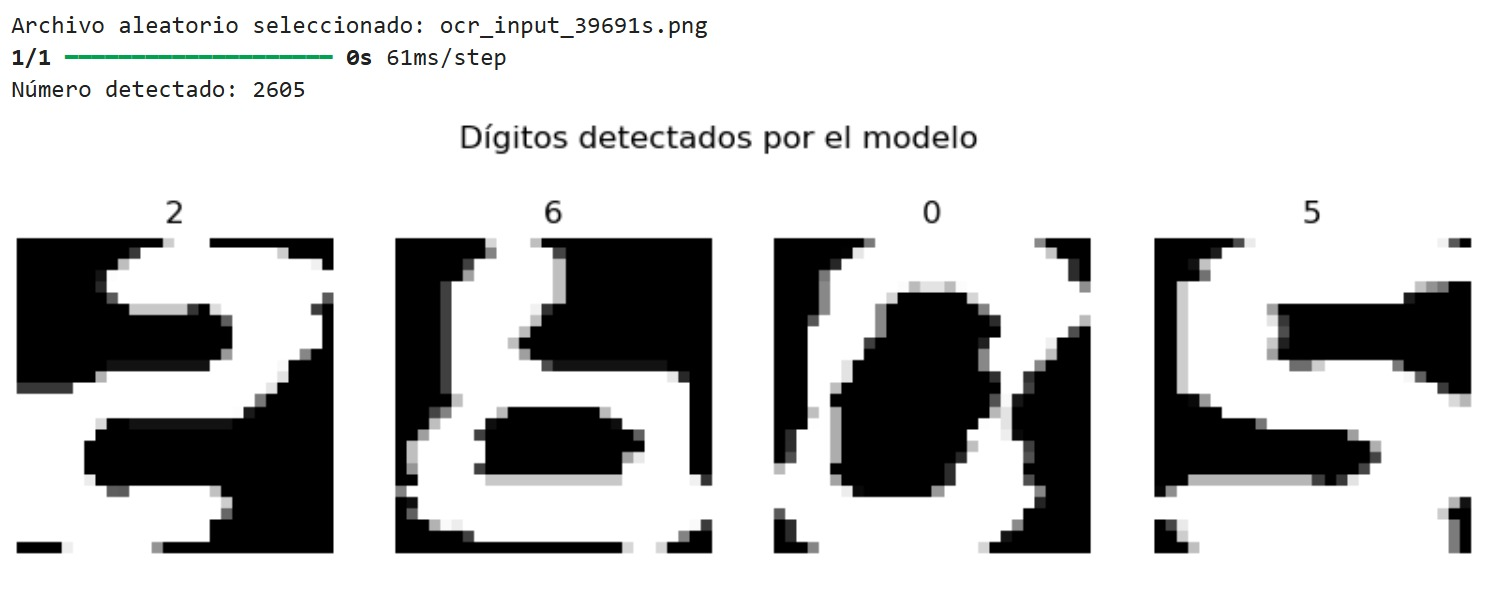
\includegraphics[width=0.9\linewidth]{../Imagenes/Foto1.jpeg}
	\end{center}
\end{minipage}	
\hfill
\begin{minipage}[t]{0.45\linewidth}
\begin{center}
	\captionof{figure}{Fotograma analizado por la red neuronal.}  
	\label{Fig:foto2}
	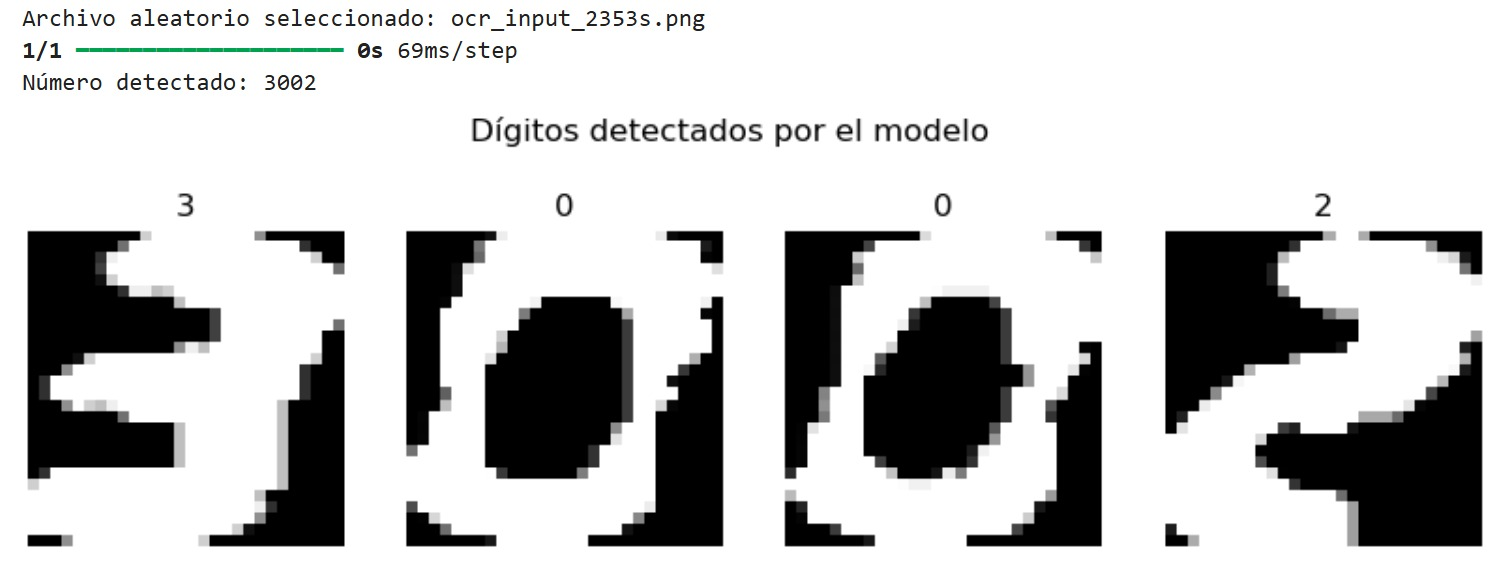
\includegraphics[width=0.9\linewidth]{../Imagenes/Foto2.jpeg}
\end{center}
\end{minipage}	

\vspace{1em}

Tras tratar los 5250 fotogramas, y realizar los histogramas de 1 segundo y 2 segundos (y luego de 5 y 10, para comprobar que tiende a una gaussiana) nos dimos cuenta de que la media de cuentas está en 8.15 (\cref{Fig:1s}), mientras que en el guión \cite{P2} se nos indica que <<(...) la media de coincidencias sea baja, inferior a 5 coincidencias>>. Por suerte teníamos una red neuronal ya entrenada, por lo que solo tuvimos que ocoger los fotogramas correspondientes a 0.1 segundos (para asgurarnos que la medida era menor a 5). Así, con más de 52500 datos, obtuvimos el histograma de 0.1 seg. (\cref{Fig:1ms}), ahora si, con una media de cuentas de 1.16, tal y como se nos pedía. 

Ahora bien, la red neuronal lee aproximadametne 52500 datos para 0.1 s y 5250 para 1 s, y en algunas ocasiones comete errores, es decir, \textbf{etiqueta un número que no sucedió, por ejemplo 7680 (pantalla) lo lee como 1680}. Esto ocurre aproximadamente con una tasa del 1\%, lo que implica aproximadamente 150 datos en 1 s. y 1500 en 0.1 ms. ¿Cómo corregimos estos datos, sin tener que revisar a mano, que al final es lo que queríamos evitar con esta red neuronal? Lo que hicimos fue un estudio estadístico de las primeras 800 cuentas (las mismas usadas para entrenar la red), de lo que deducimos un número máximo para las cuentas de 1 segundo. Este dato será el valor de corte para el valor de 1 segundo. A sabiendas de que estamos usando un corte usando el 15\% de las cuentas, lo que haremos será incrementar levemente este límite. Cuánto lo comentaremos posteriormente, y como trasladarlo a las frecuencias con otros segundos también.
 

\subsection{Límite de la Binomial a Poisson y de Poisson a Gauss}

Supongamos que nuestras medidas es analizar el número de éxitos que hay en un número de pruebas. Cada prueba es un proceso binario, ya que solo hay dos resultados: éxito o fracaso. En el caso de que el eveneto sea aleatorio con una probabilidad de éxito en cada instante 

En el análisis estadístico de los procesos de detección de radiación, es habitual modelar los eventos observables (como la detección de partículas) mediante distribuciones de probabilidad discretas. Una de las más fundamentales es la distribución binomial, la cual describe la probabilidad de observar \( x \) éxitos en \( n \) ensayos independientes, cada uno con una probabilidad de éxito \( p \): 

\begin{equation}
    P_{\text{Binomial}}(x) = \binom{n}{x} p^x (1 - p)^{n - x}
\end{equation}
Cuando uno estudia fenómenos que sigan este esquema en el que la probabildiad de éxito es muy pequeña y el número de fenómenos estudiados es elevado, la distribución binomial puede aproximarse por una distribución de Poisson. Para que la binomial tienda a una distribución de Poisson, se deben cumplir las siguientes condiciones:

\begin{itemize}
    \item \( n \to \infty \) (número de ensayos muy grande).
    \item \( p \to 0 \) (probabilidad de éxito muy pequeña).
    \item \( \mu = np = \text{constante} \) (media finita y fija).
\end{itemize}

En este límite, la distribución binomial converge a:

\begin{equation}
	P_{\text{Poisson}}(x) = \frac{(\mu)^x}{x!} e^{-\mu}
\end{equation}
donde $\mu$ es la \textit{media} de la distribución (ec. 3.24 \cite{Knoll:1300754}). Por otro lado, cuando el número esperado de eventos \( \mu \) es suficientemente grande (\( \mu \gtrsim 30 \)), la distribución de Poisson puede aproximarse por una distribución normal (o gaussiana), gracias al teorema del límite central:

\begin{equation}
	P_{\text{Gauss}} (x) = \frac{1}{\sqrt{2\pi \mu}} \exp \parentesis{- \frac{(x-\mu)^2}{\mu}}
\end{equation}
donde de nuevo $\sigma=\sqrt{\mu}$. En esta sección nos centraremos en estudiar las caracaterísticas estadísticas de la radiación cósmica en diferentes intervalos de tiempo. Así, seremos quienes de afirmar si para un tiempo determinado de medida la distribución sigue (o no) una distribución de binomial, de Poisson y/o Gauss. 

\subsubsection{Chi cuadrado de la distribución}

Sea $N$ el número de cuentas, $h(x_i)$ la frecuencia observada de la medida $x_i$, $P(x_i)$ y $NP(x_i)$ la distribución de probabilidad y la predicción de una distribución particular (Gauss o Poisson)

\begin{equation}
	\chi^2_{\text{Poisson}} = \sum_{i=0}^N \frac{(h(x_i)-NP(x_i))^2}{\sigma(x_i)^2} \qquad 
	\chi^2_{\text{Gauss}}= \sum_{i=0}^N \frac{(h(x_i)-NP(x_i))^2}{\sigma(x_i)^2} \qquad 
\end{equation}
véase Bevington \cite{Bevington:1305448} donde $i$ recorre todos los posibles datos. El valor $\sigma(x_i)=\sqrt{(NP(x_i))}$, que en el bevington aproximan por $\sigma(x_i)\approx \sqrt{h(x_i)}$. Nosotros usaremos esta última ya que <<the flucutations in the observed frequencies $h(x_j)$ come from the statistical probabilities of making random selections of finite numbers of items and are distributed according to the Poisson distribution (...)>>. Comprobando si $\chi^2$ es mayor o menor que el valor tabulado, veremos la compatibilidad de los datos con la distribución en cuestión. \textbf{Los grados de libertad} serán siempre el número de bins menos 2, siendo estos dos las dos ligaduras de las distribuciones: la normalización de la distribución y la media.

\subsection{Análisis: error cometido por la red neuronal.}

Los valores contados a mano son: 

\begin{center}
\begin{table}[H]
\caption{Tabla para 1 s con $\mu=7.63$, $N=865$, $\chi^2_{\text{Poisson}}=18.30$  y $\chi^2_{\text{Gauss}}=35.48$}
\label{Tab:histo_manual_1s}
\begin{tabular}{cccccccc}
\toprule
 & $h(x_j)$ & $N \cdot P_{\text{poisson}} (x_j)$ & $\chi^2_{\text{poisson}}(x_j)$ & $N \cdot P_{\text{gauss}} (x_j)$ & $\chi^2_{\text{gauss}}(x_j)$ \\
\midrule
0-1 & \num{    7} & \num{4.06} & \num{1.24} & \num{12.54} & \num{4.38} \\
2 & \num{   13} & \num{12.26} & \num{0.04} & \num{15.68} & \num{0.55} \\
3 & \num{   36} & \num{31.17} & \num{0.65} & \num{30.71} & \num{0.78} \\
4 & \num{   51} & \num{59.42} & \num{1.39} & \num{52.76} & \num{0.06} \\
5 & \num{   99} & \num{90.64} & \num{0.71} & \num{79.49} & \num{3.84} \\
6 & \num{  108} & \num{115.21} & \num{0.48} & \num{105.06} & \num{0.08} \\
7 & \num{  145} & \num{125.52} & \num{2.62} & \num{121.78} & \num{3.72} \\
8 & \num{  100} & \num{119.66} & \num{3.87} & \num{123.82} & \num{5.67} \\
9 & \num{   90} & \num{101.40} & \num{1.44} & \num{110.42} & \num{4.63} \\
10 & \num{   85} & \num{77.33} & \num{0.69} & \num{86.37} & \num{0.02} \\
11 & \num{   58} & \num{53.62} & \num{0.33} & \num{59.26} & \num{0.03} \\
12 & \num{   27} & \num{34.08} & \num{1.85} & \num{35.66} & \num{2.78} \\
13 & \num{   18} & \num{19.99} & \num{0.22} & \num{18.82} & \num{0.04} \\
14 & \num{   13} & \num{10.89} & \num{0.34} & \num{8.71} & \num{1.41} \\
15 & \num{    7} & \num{5.54} & \num{0.31} & \num{3.54} & \num{1.71} \\
16-21 & \num{    9} & \num{4.63} & \num{2.12} & \num{1.79} & \num{5.77} \\
\bottomrule
\end{tabular}
\end{table}
\end{center}


\begin{figure}[h!] \centering
	\caption{Histograma para 1 s. con datos tomados a mano.}
	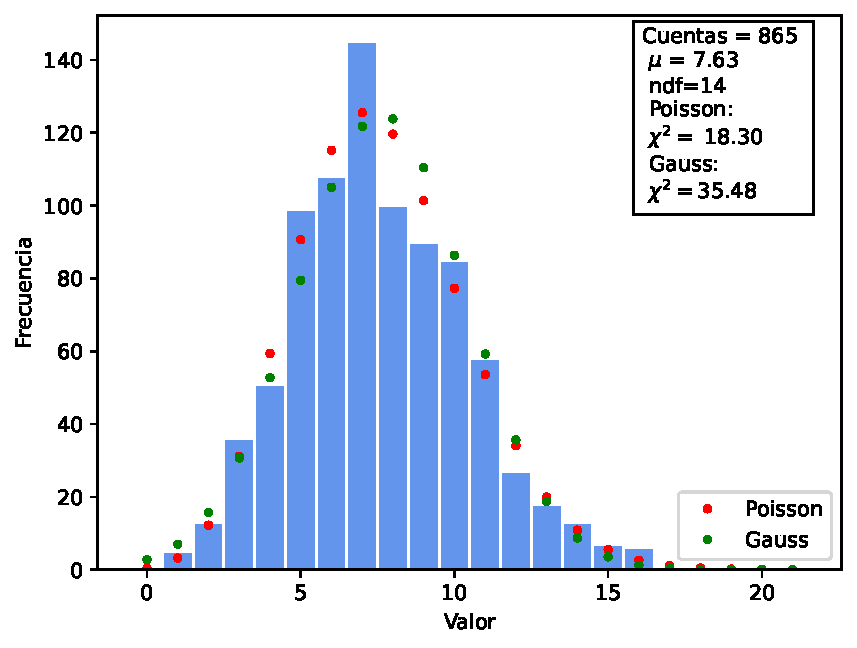
\includegraphics[width=0.5\linewidth]{../Graficas/Histo_1manuals.pdf}
\end{figure}
donde podemos ver que hemos juntado los valores totales posibles para aquellas cuentas inferiores a 5 ya que ``si la media de cuentas por intervalo es pequeña ($\leq$5), en la distribución de Poisson muestra su carácter discreto y asimétrico, y es preferible reagrupar los bins antes de aplicar un test'' \cite{P2}. La frecuencia entre 0-1 y 16-21 cuentan cada uno como un único grado de libertad. Para la evalución de la probabilidad claramente $P\cdot N$ tenemos claramente que sumar la probabilidad de 0 y 1 para tener la de 0-1, idém para 16-21. Aunque reduce la resolución del histograma, este proceso mejora la validez estadística. Este proceso lo seguiremos en todas y cada una de las gráficas posteriores. 

Los valores de la $\chi^2$ para ambas distribuciones no dejan margen de duda (tabulación procedente del \href{https://www.itl.nist.gov/div898/handbook/eda/section3/eda3674.htm}{NIST}). La $\chi^2_{0.9,14}=21.064$, tal que nuestra distribución de poisson $\chi^2_{\text{Poisson}}=20.58$, por lo que podemos afirmar que sigue dicha distribución con una alta probabilidad, mientras que $\chi^2_{\text{gauss}}=58.15$, lo que es descartable con un margen de confianza altísimo ya que $.\chi^2_{0.999,14}=36.123$.

Los datos avalan un comportamiento claramente poissoniano, por lo que podemos usar la distribución de Poisson para dar un margen máximo a la distribución. Por ejemplo, para la distribución de poisson con media 7.63, aseguramos que un valor por encima de 30 tiene a un 0.0000001 de posibilidades (10$^{-6}$). Para el resto haremos lo mismo, es decir, para 0.1 seg. el límite estará en $k=4$, para 0.2 seg. estará en $k=7$... calculado a partir de la distribución con la media $\mu$ de dicha distribución

Dado que lo que queremos estudiar es la distribución de Poisson, será suficiente comprobar si los datos entre esos límites se ajustan o no a la misma distribución, ya que aunque haya más datos fuera de la distribución, podremos asumirlos como fallos de la red neuronal, y descartarlos como \textbf{errores sistemáticos}. El número de cuentas usada para normalizar las distribuciones serán el número de cuentas encerradas por estos límites (0,k).

\subsection{Análisis: estudio de las distribuciones}

Aquí nos limitaremos a comentar con que grado de confianza son compatibles los diferentes resultados. Son valores tabulados fueron tomados del \href{https://www.itl.nist.gov/div898/handbook/eda/section3/eda3674.htm}{NIST}. Hemos aplicado a todas las distribuciones el mismo proceso que el anterior. Las tablas para los cálculos de la $\chi^2$ las colocamos en el apéndice \ref{Sec:tablas}, ya que colocarlas aquí nos llevaría a un problema de espacio bastante grande. 


\begin{itemize}
	\item \textbf{Cuentas de 0.1s}: como podemos ver el valor de la $\chi^2$ tanto para la gaussiana como para la poissoniana excede por muchísimo los valores razonables que cabría esperar para un $\chi_{0.999,3}=18.467$. Consecuentemente queda descartada la hipótesis nula: nuestros números de cuentas cada 0.1 s no siguen una distribución poissoniana o gaussiana (con $\alpha=99.9$\%).
	\item \textbf{Cuentas de 0.2s}: al superar el valor tabulado $\chi_{0.999,6}=22.458$ podemos afirmar que nuestors valores no siguen dichas distribuciones (con $\alpha=99.9$\%).
\end{itemize}
	\begin{minipage}[t]{0.5\linewidth}
		\begin{center}
		\captionof{figure}{Frecuencia para las cuentas en 0.1s}  
		\label{Fig:1ms}
		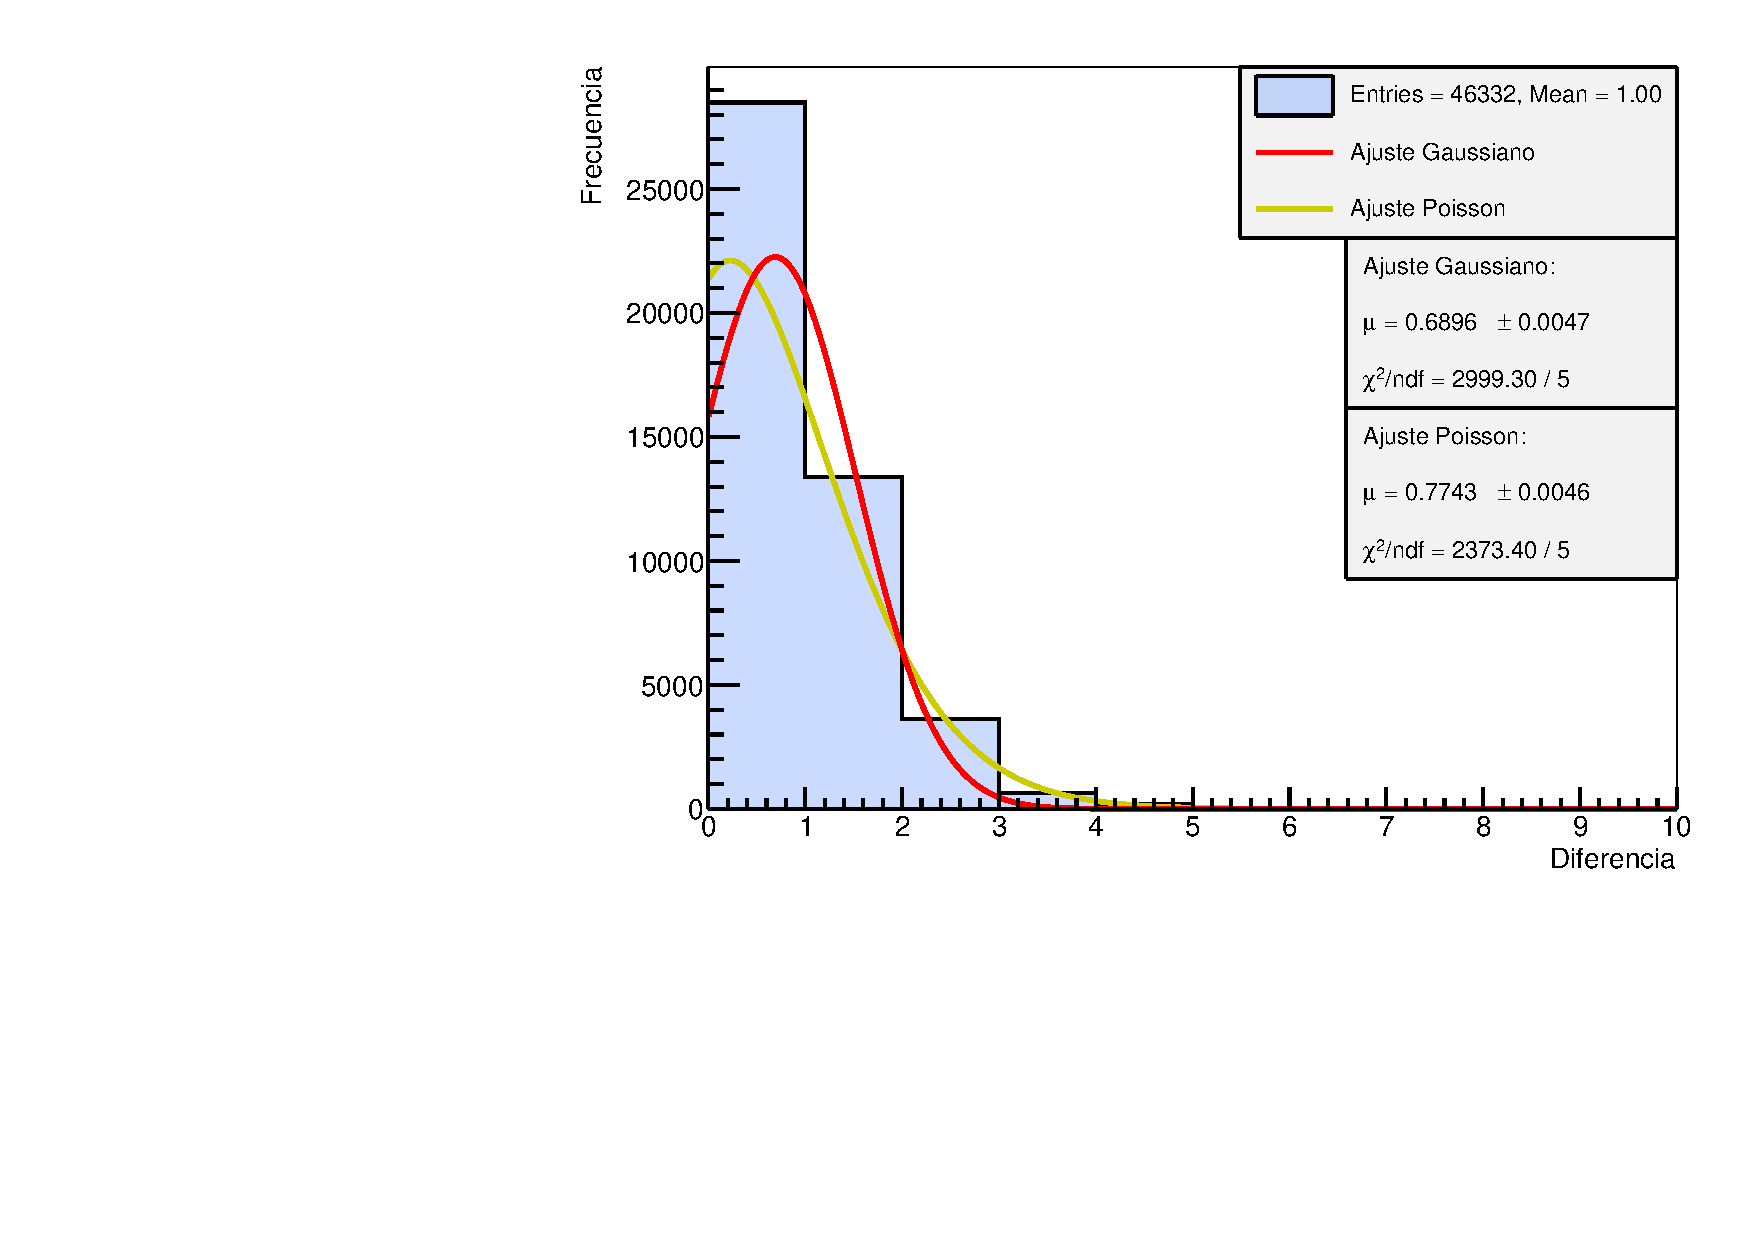
\includegraphics[width=1\linewidth]{../Graficas/Histo_1ms.pdf}
		\end{center}
	\end{minipage}	
	\hfill
	\begin{minipage}[t]{0.5\linewidth}
	\begin{center}
		\captionof{figure}{Frecuencia para las cuentas en 0.2s}  
		\label{Fig:2ms}
		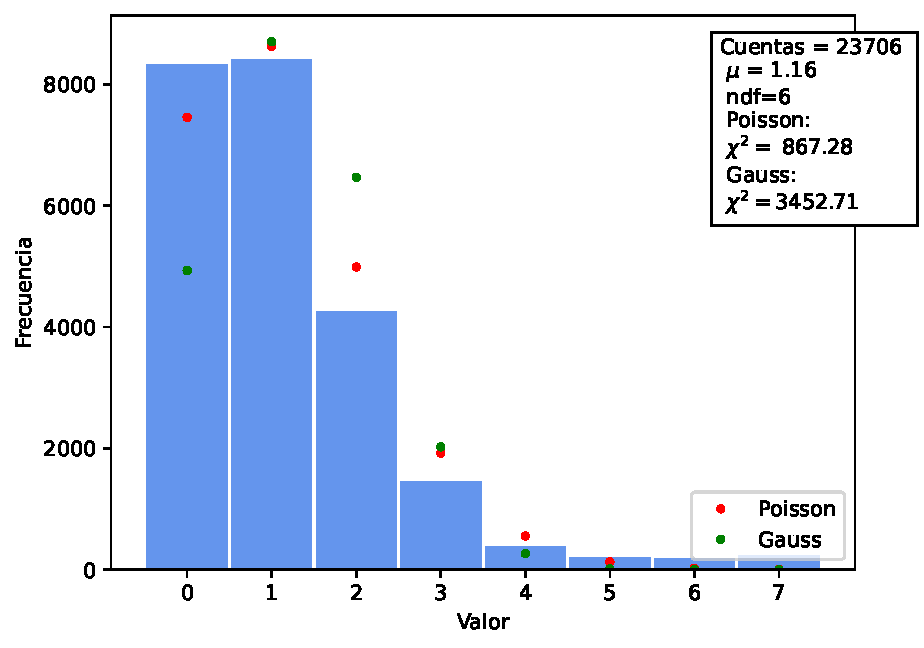
\includegraphics[width=1\linewidth]{../Graficas/Histo_2ms.pdf}
	\end{center}
	\end{minipage}	
	

\begin{itemize}
	\item \textbf{Cuentas de 0.5s}: el valor de la chi cuadrado sigue sobrepasando los límites tabuldados ya que $\chi_{0.999,12}= 32.910$, por lo que podemos afirmar que nuestors valores no siguen dichas distribuciones (con $\alpha=99.9$\%).
	\item \textbf{Cuentas de 0.7s}: al superar el valor tabulado $\chi_{0.999,14}=36.123$ podemos afirmar que nuestors valores no siguen dichas distribuciones (con $\alpha=99.9$\%).
\end{itemize}


\begin{minipage}[t]{0.5\linewidth}
\begin{center}
	\captionof{figure}{Frecuencia para las cuentas en 0.5s}  
	\label{Fig:5ms}
	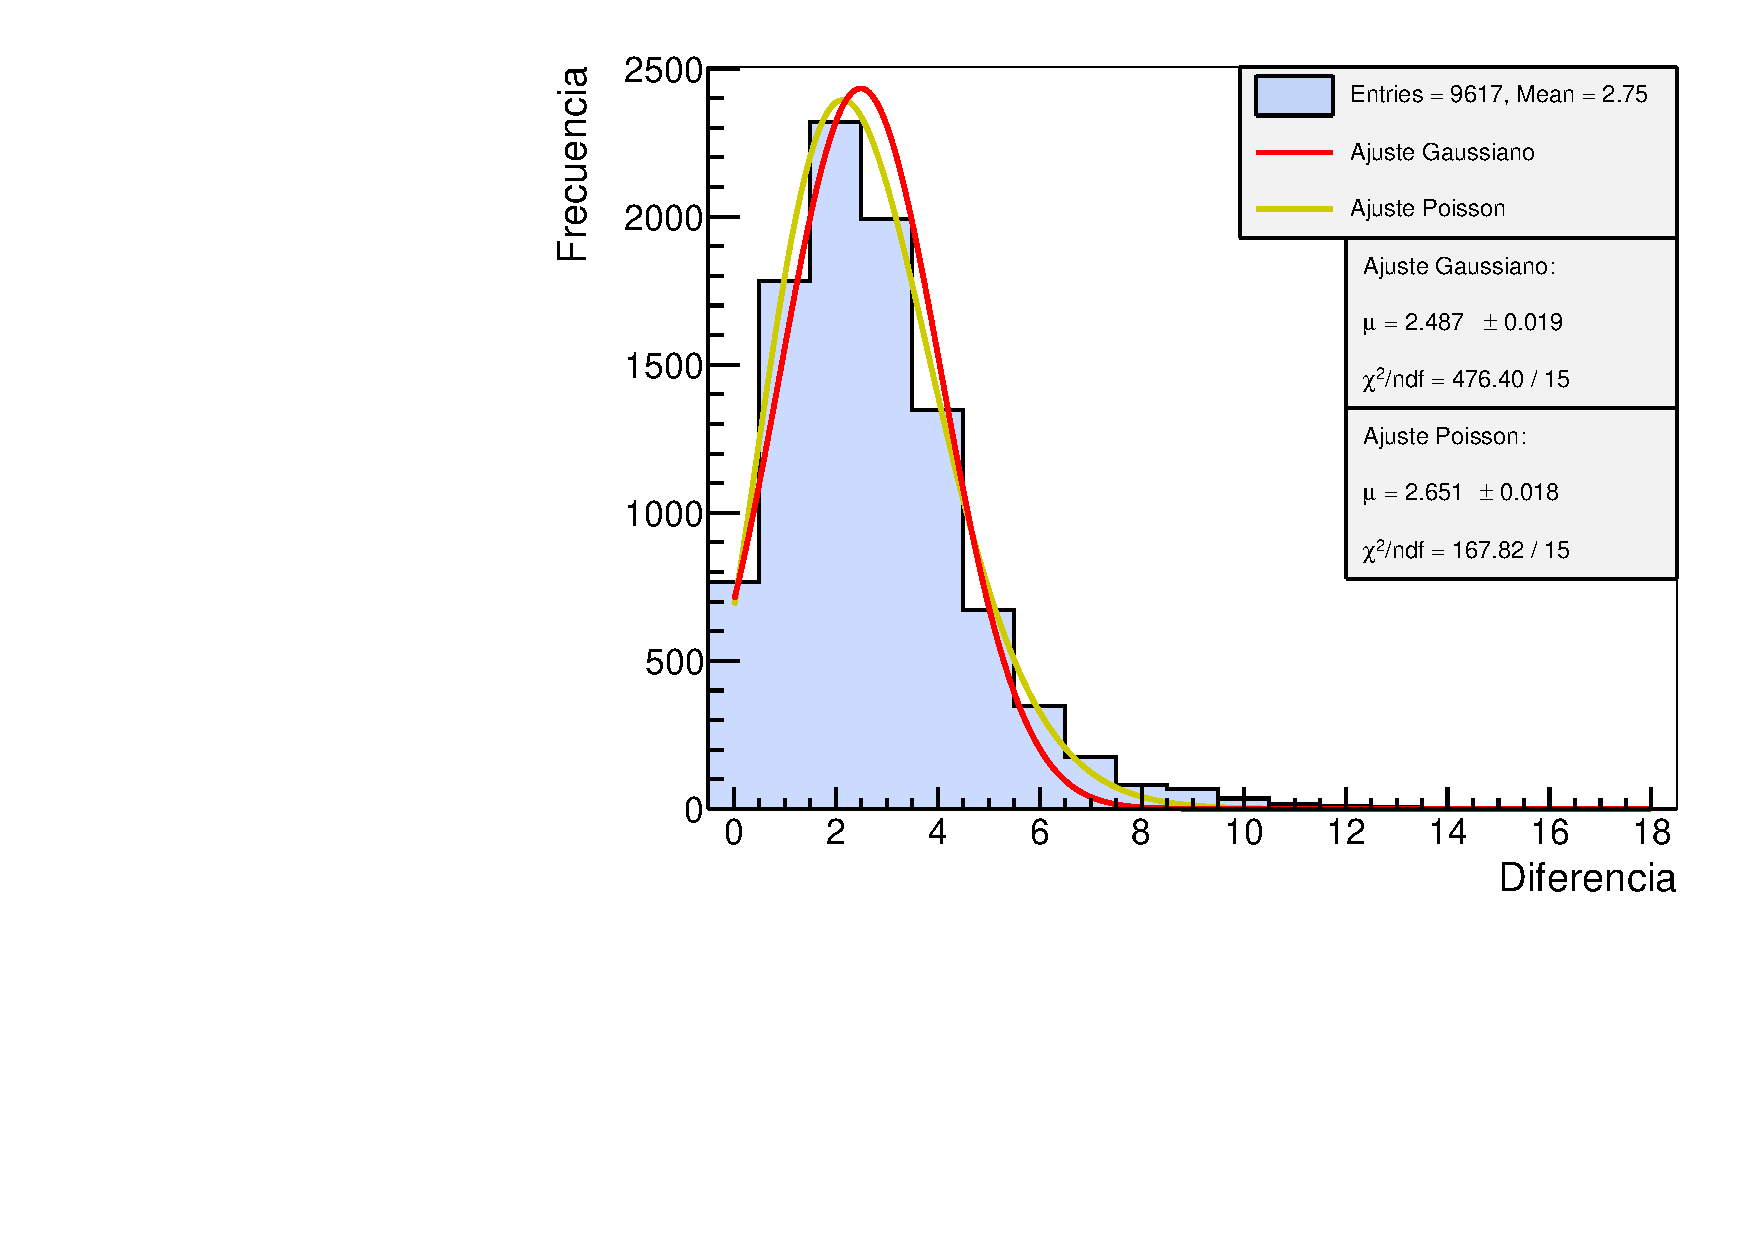
\includegraphics[width=1\linewidth]{../Graficas/Histo_5ms.pdf}
\end{center}
\end{minipage}	
\hfill
\begin{minipage}[t]{0.5\linewidth}
\begin{center}
	\captionof{figure}{Frecuencia para las cuentas en 0.7s} 
	\label{Fig:7ms}
	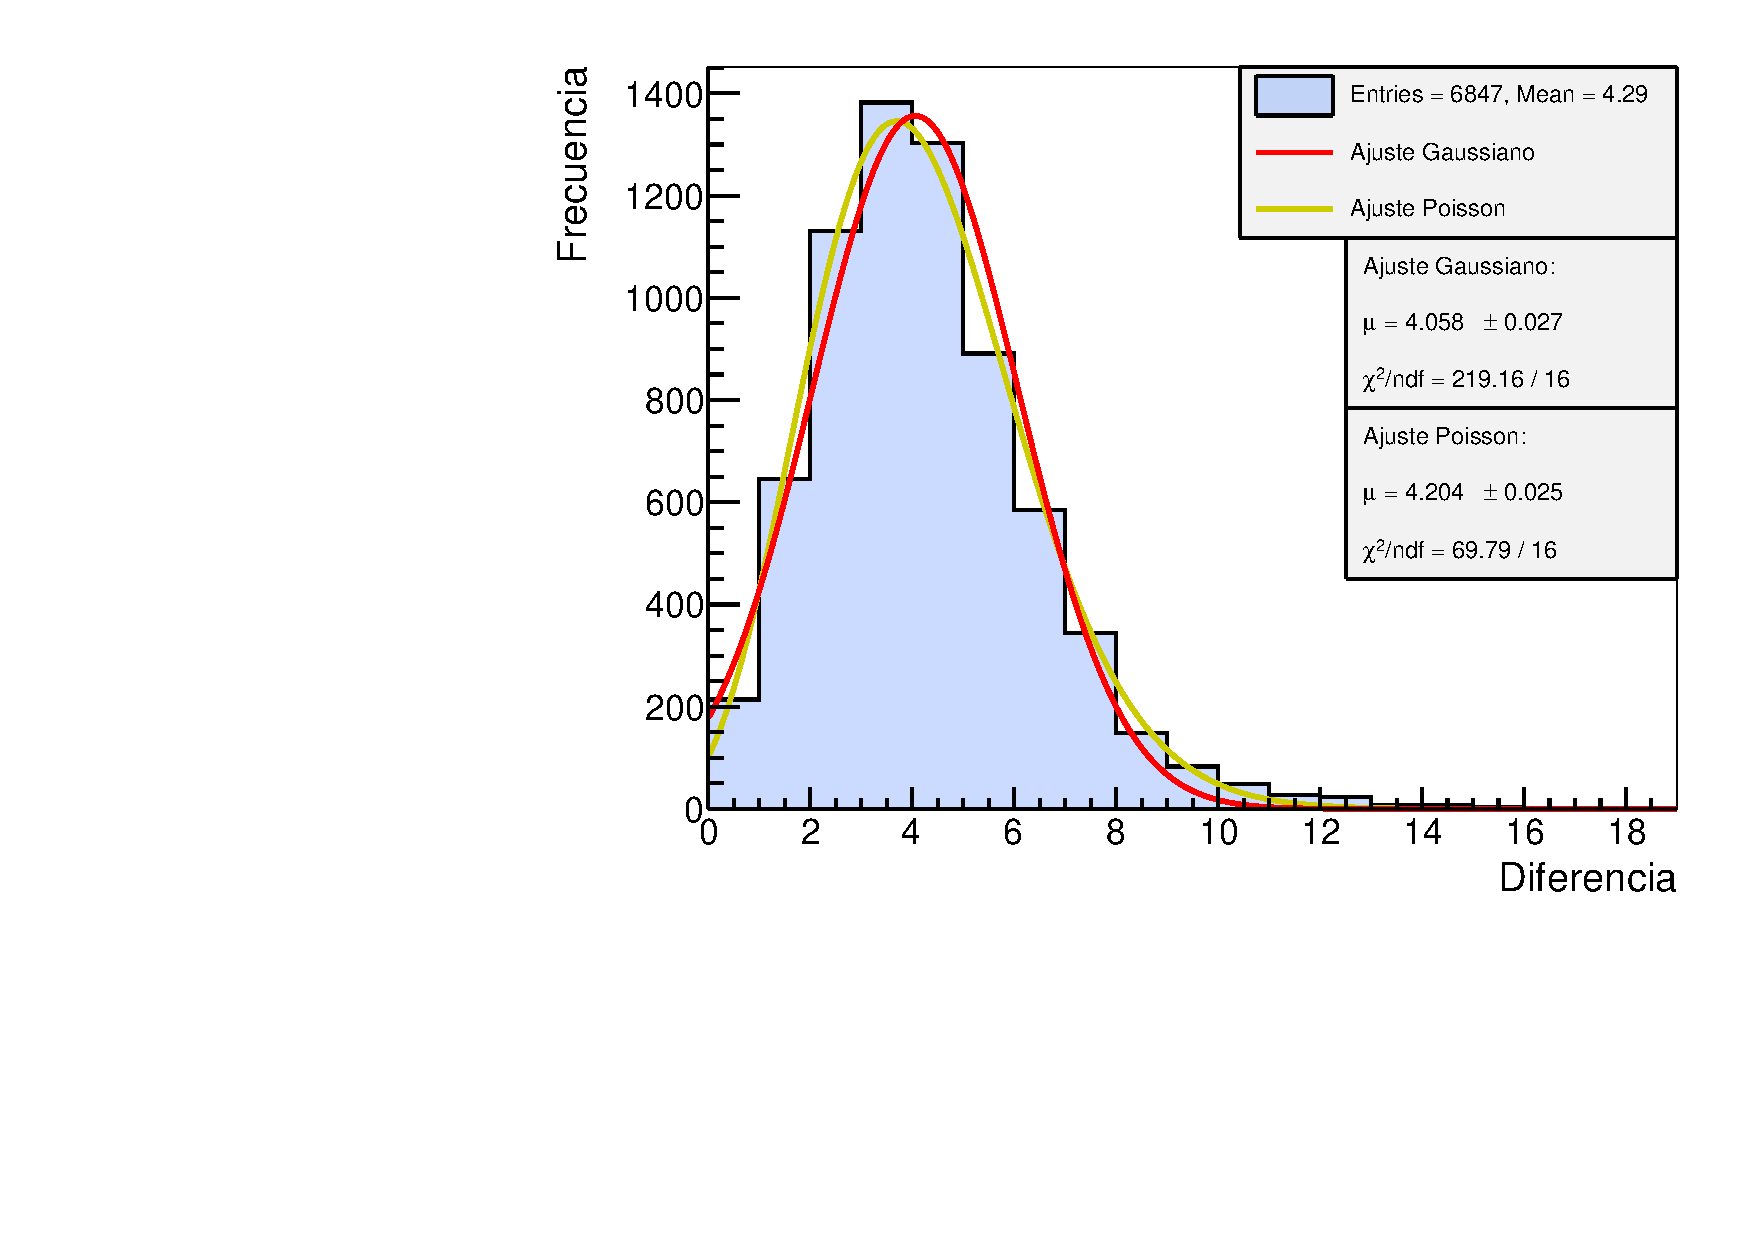
\includegraphics[width=1\linewidth]{../Graficas/Histo_7ms.pdf}
\end{center}
\end{minipage}	



\begin{itemize}
	\item \textbf{Cuentas de 1s}: el valor de la chi cuadrado tabulado para $\alpha=0.999\%$ y 19 grados de libertad es  $\chi_{0.999,19}=43.820$, por lo que nuestro ajuste poissoniano es descartable con este nivel de confianza, también nuestro ajuste gaussiano.
	\item \textbf{Cuentas de 2s}: el valor de la chi cuadrado tabulado para $\alpha=0.999\%$ y 18 grados de libertad es  $\chi_{0.999,23}=49.728$, por lo que nuestro ajuste poissoniano no es descartable con este nivel de confianza, y tampoco nuestro ajuste gaussiano.Aún así nuestro ajuste poissoniano y gaussiano es mayor que el valor tabulado para un 99\% de confianza $\chi_{0.9,23}=41.638 $, por lo que es descartable para un alto nivel de confianza, pero no tanto como las anteriores distribuciones. 
\end{itemize}
\begin{minipage}[t]{0.5\linewidth}
	\begin{center}
	\captionof{figure}{Frecuencia para las cuentas en 1s} \label{Fig:1s}
	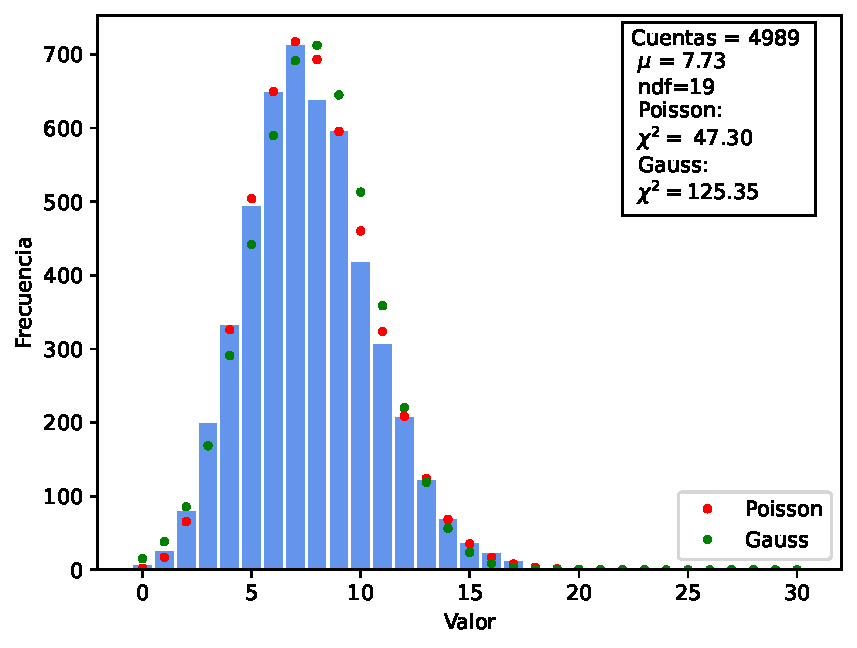
\includegraphics[width=1\linewidth]{../Graficas/Histo_1s.pdf}
	\end{center}
\end{minipage}	
\hfill
\begin{minipage}[t]{0.5\linewidth}
\begin{center} 
	\captionof{figure}{Frecuencia para las cuentas en 2s}\label{Fig:2s}
	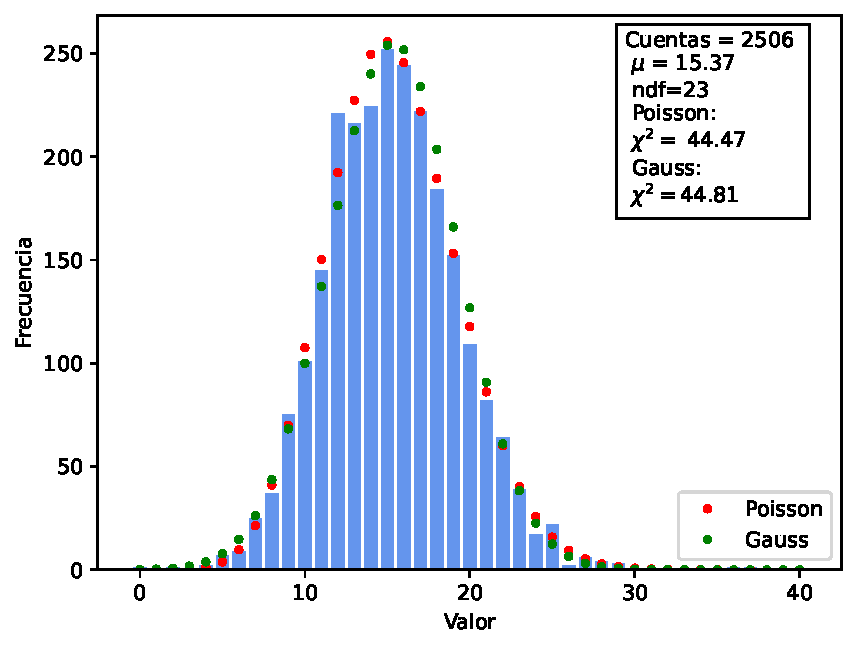
\includegraphics[width=1\linewidth]{../Graficas/Histo_2s.pdf}
\end{center}
\end{minipage}	

\begin{itemize}
	\item \textbf{Cuentas de 5s}: la distribución de poisson verifica $\chi_{0.9,28}=37.916$, por lo que no es descartable. La gaussiana además está por debajo de $\chi_{0.975,28}=44.461$, por lo que la distribución empieza a ser valida. 
	\item \textbf{Cuentas de 10s}: las distribuciones (tanto para gauss como para Poisson) verfican que $\chi^2<\chi_{0.9,31}=41.422$, por lo qeu ambas son buenas distribuciones. En este caso incluso la distribucción gaussiana tiene una $\chi^2$ menor que la Poissoniana. 
\end{itemize}

\begin{minipage}[t]{0.5\linewidth}
\begin{center}
		\captionof{figure}{Frecuencia para las cuentas en 5s} \label{Fig:5s}
		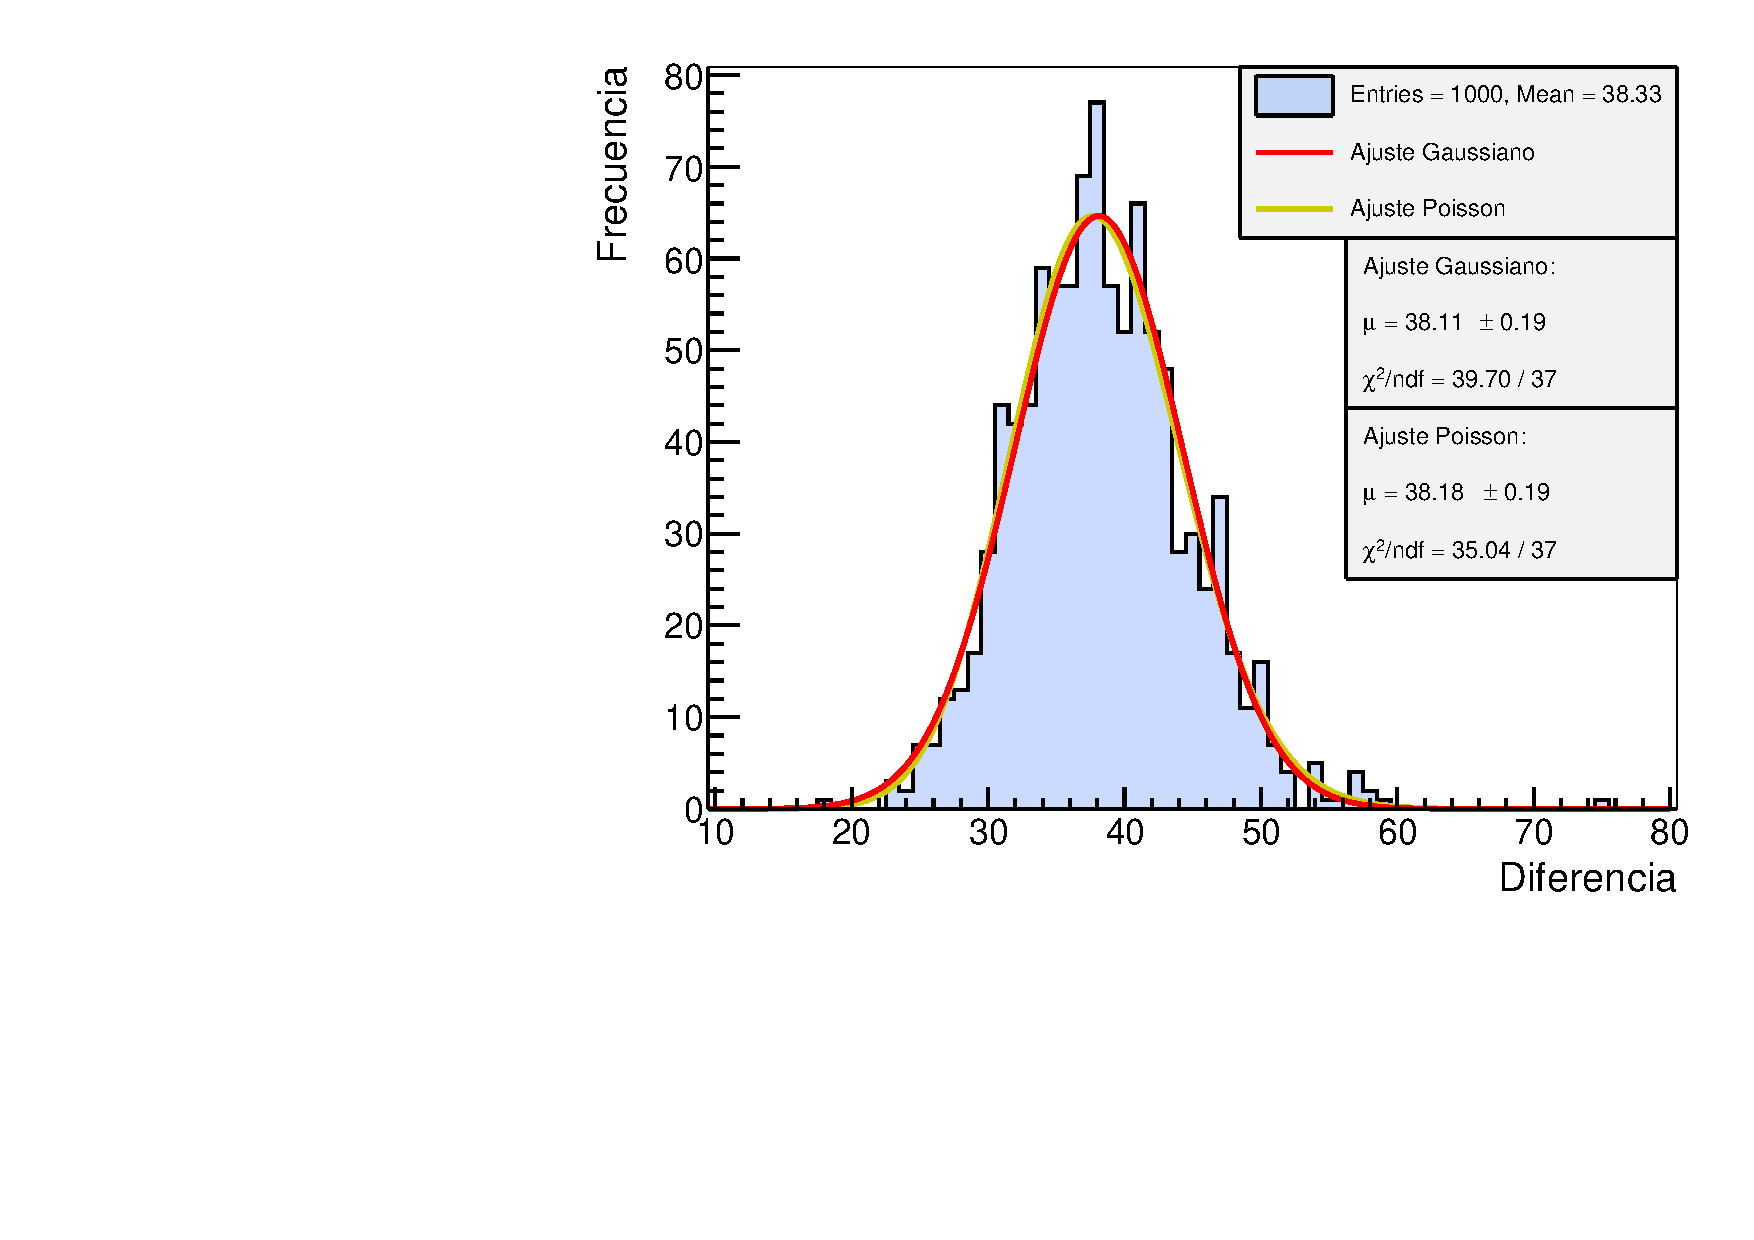
\includegraphics[width=1\linewidth]{../Graficas/Histo_5s.pdf}
\end{center}
\end{minipage}	
\hfill
\begin{minipage}[t]{0.5\linewidth}
\begin{center}
		\captionof{figure}{Frecuencia para las cuentas en 10s} \label{Fig:10s}
		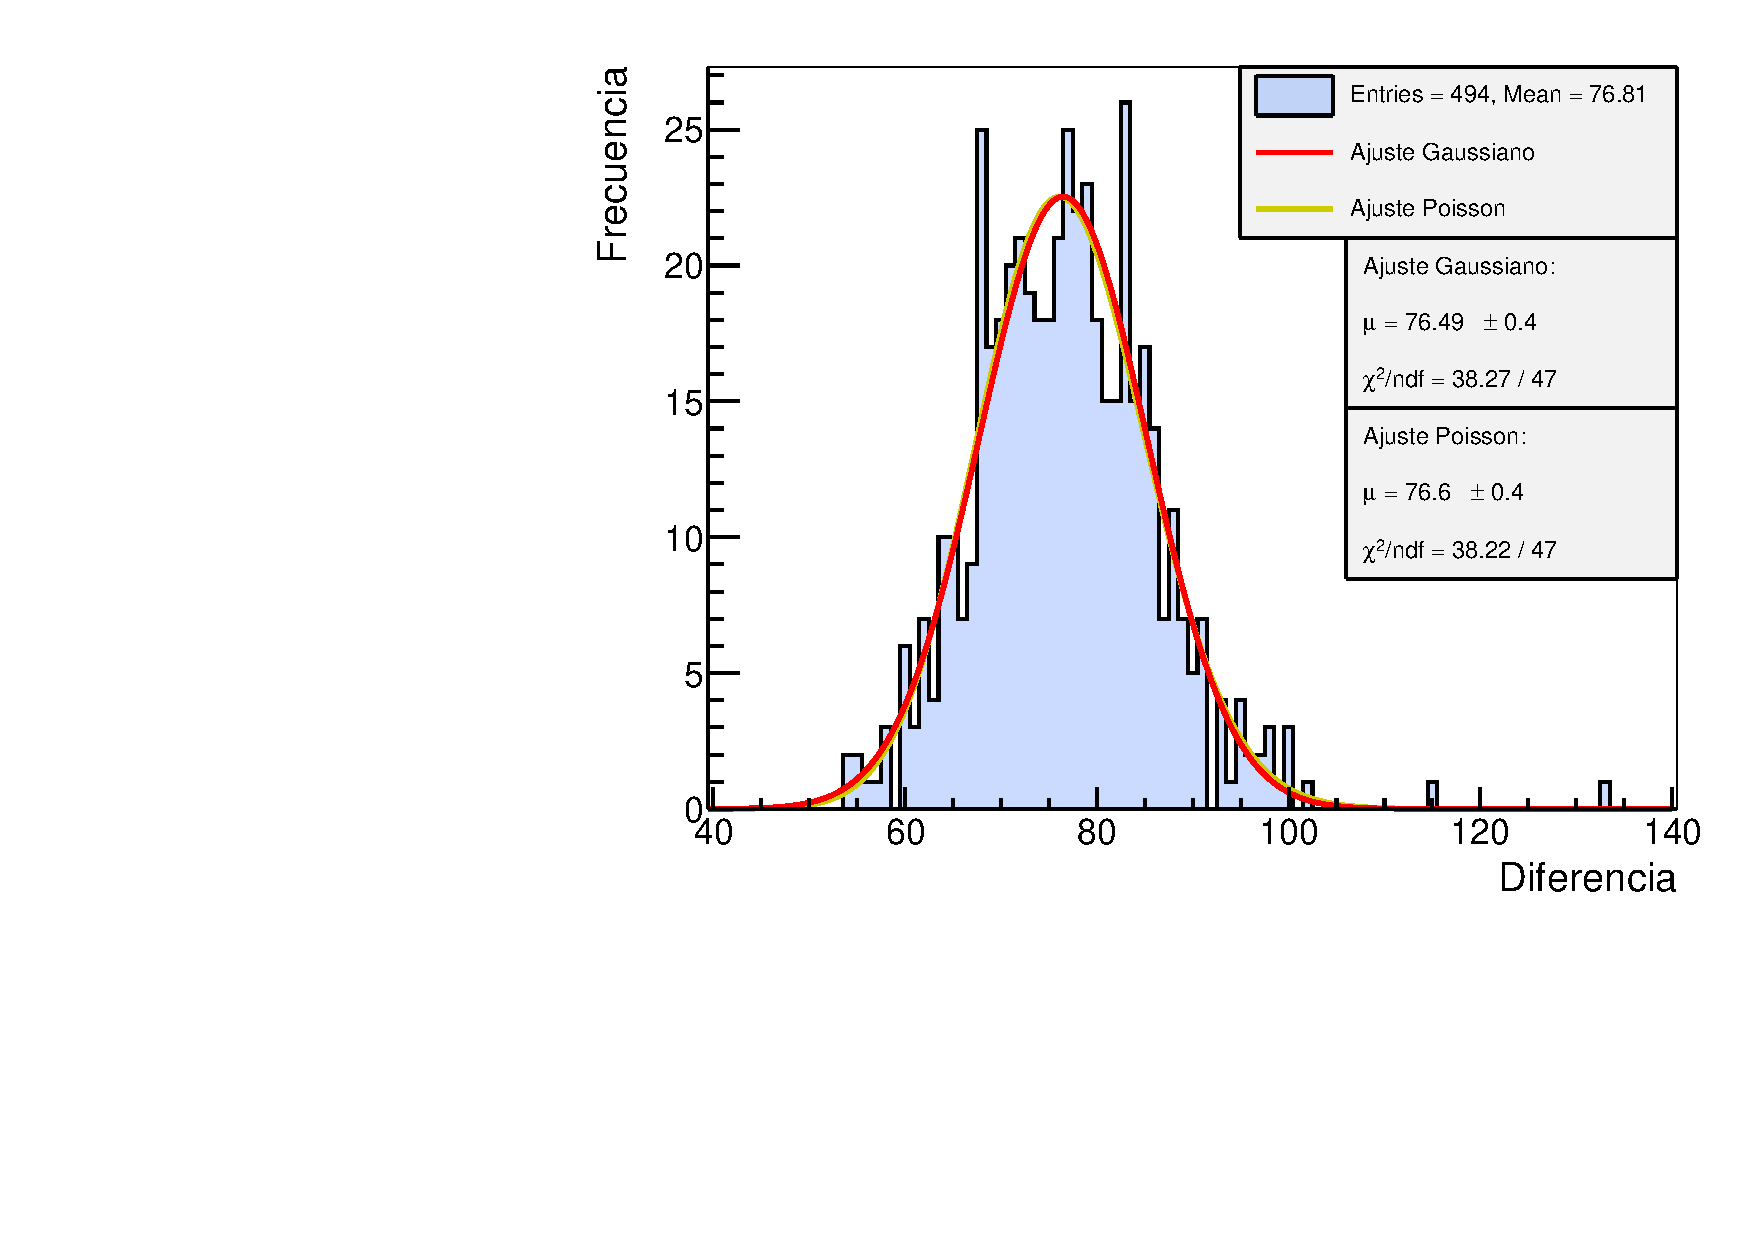
\includegraphics[width=1\linewidth]{../Graficas/Histo_10s.pdf}
\end{center}
\end{minipage}	

\subsection{Conclusiones}

Lo primero que nos llama la antención es la diferencia de $\chi^2$ entre la distribución de 1 seg. contada manualmente y contada con la ia. Es claro que la red neuronal comete un error sistemático que nosotros no podemos controlar (faltaría más entrenamiento, mejor resolución del vídeo...) y que nosotros al realizar el contaje a manualmente no cometemos. Lógicamente si el resultado de la $\chi^2$ manual y por red neuronal fuera igual, podríamos dudar acerca de este error, sin embargo para unas cuentas los datos siguen la distribución Poissoniana y en otros no. Esta diferencia nos lleva a la conclusión de que quizás necesitamos más entrenamiento para la red, y una comparación con mucho más datos. 

Quizás si fueramos capaces de comparar los primreos 850 datos manuales y por red neuronal seríamos quienes de cuantificar este error sistemático, de dar una solución y evidentemente respaldar mucho más los datos y su método de obtención. Sería una gran mejora para una futura revisión de la memoria.


En cualquier caso, lo que está claro es que a partir de varios segundos la distribución de las cuentas empieza a ser una Poissoniana/Gaussiana, lo cual nos hace afirmar que $\sigma(N)=\sqrt{N}$ para el número de cuentas. 


\section{Atenuación de la radiación cósmica secundaria}

En esta sección vamos a obtener cuanta de la radiación cósmica incidente pertenece a la parte dura (muones) y cuanta a la parte blanda (electrones, positrones). Cada una de estas llegará con una energía a nuestro detector dependiente del camino recorrido y su interacción con el aire (que depende, por ejemplo, de la masa de la partícula) por lo que tendrán diferentes distribuciones de energía al llegar a nuestro detector. Sin embargo nuestro aparato de medida no puede diferenciar con que energía llega la partícula, solo detecta las cuentas, por lo que el descarte a través de la energía es imposible. 

Una de las maneras podría ser reducir la tasa electrónica o muónica a prácticamente cero, por ejemplo colocando poniendo un material justo encima de nuestro detector sin reducir la otra componente de las coincidencias. De esta manera podríamos inferir de ahí un valor aproximado de una de las componentes, y por diferencia con la tasa sin ningún material, ambas componentes. Este es precisamente el método que vamos a usar, ya que el recorrido libre medio másico del electrón es mucho menor que el del muón. En resumen: a través de la colocación de planchas de diferentes metales vamos a tratar de reducir al máximo el valor de la componente electrónica , obteniendo así un valor para la tasa muónica. 

Para estudiar esto necesitamos unas nociones básicas sobre el comportamiento de estas dos partículas en cada material. La atenuación de los rayos cósmicos secundarios puede simplificarse en promedio a través del recorrido libre medio másico, $\lambda_ m^{\mu}$ para los muones y $\lambda_m^e$ para los electrones, donde el número de partículas $N(x)$ que sobreviven tras atravesar el espesor es: 

\begin{equation}
	N(x)  = N(0) e^{-x\rho/\lambda}
\end{equation}
siendo $N(0)$ el número de partículas incidentes sobre dicho material. \textcolor{blue}{Esta expresión es válida para describir la atenuación de partículas cargadas en materiales cuando se puede considerar que la probabilidad de interacción por unidad de masa es constante. Esto se cumple para partículas relativistas como muones y electrones de rayos cósmicos secundarios, cuya trayectoria es esencialmente rectilínea y cuya pérdida de energía ocurre de forma continua.}

En este contexto, el recorrido libre medio másico $\lambda$ representa la cantidad de masa que una partícula recorre, en promedio, antes de ser atenuada. Como la atenuación depende exponencialmente del producto $x\rho$, esta expresión permite estimar experimentalmente la reducción de flujo al interponer materiales densos. 

La diferencia entre $\lambda_\mu=100$ g/cm$^2$ y $\lambda_e=1550$ g/cm$^2$ es suficientemente grande como para que uno se atenue significativamente y el otro no. Como podemos ver en la ecuación anterior, la atenuación es significativamente mayor con un material muy denso que con uno poco denso, por lo que nosotros usaremos láminas de hierro $\rho$(Fe)$=7.874$ g/cm$^3$ y láminas de plomo $\rho$(Pb)$=11.340$ g/cm$^3$. 

Así pues, solo tendremos que realizar diferentes regresiones exponenciales de los valores de las tasas reales frente al espesor $x$ de los diferentes materiales para obtener así tanto $n(0)$ como $\lambda$. Si $x$ es el grosor total de las placas colocadas encima del detector (tratando de superponerse lo máximo posible) y $n_r$ la tasa real, tenemos que los parámetros $a$ y $b$ ajuste exponencial siguiente

\begin{equation}
	n_r = a e^{-bx}
\end{equation}
se relacionan con los valores que queremos obtener de la siguiente manera:

\begin{equation}
	a = n_r(0) \qquad b = \frac{\rho}{\lambda} \rightarrow \lambda_m = \frac{\rho}{b}
\end{equation}



\subsection{Láminas de hierro}

Primero empezamos colocando plancas de hierro de espesor $x_{\text{Fe}}=1.600(14)$ mm, de dos en dos ya que teníamos 20 planchas y un tiempo limitado. Las incertiumbre total de $n$ planchas lo calculamos como $u(n\cdot x) = n \cdot u(x)$, ya que la incertidumbre del grosor de cada una de las planchas tiene la misma fuente de incertidumbre: la precisión del calibre, y por tanto no son independientes. \textcolor{blue}{No usamos incertidumbre de tipo A dado que ya no tenemos la posibilidad de medir las planchas, aunque debiera hacerse, ya que con la incertidumbre usada no estamos teniendo en cuenta posibles diferencias entre placas de hierro/plomo, diferencia de espesores en una y otra región (ya que estaban bastante magulladas)... Además de las distancias entre una placa y otra en las que había aire (no estan completamente pegadas). Estos factoers que se deberían haber estudiado como incertidumbre de tipo A al no poder ser modelizadas. Consecuentemente la incertidumbre que debieramos tener en cuenta en un estudio posterior del grosor es mucho mayor que el previamente descrito} 

En la \cref{Fig:hierro} vemos los datos de la \cref{Tab:hierro} representados gráficamente con el ajuste exponencial comentado anteriormente hecho. \textcolor{blue}{Como podemos ver en esta tabla hay varios conjuntos de datos para la misma distancia. ¿Por qué están separados y no juntos? En primer lugar fueron medidos en instantes diferentes del día (en general con una separación de 1 hora), que en el caso de la radiación cósmica puede provocar diferencias. Además de esto, estos datos fueron tomados en diferentes configuraciones experimentales (diferntes posiciones de la lona, orden de las planchas...), por lo que en realidad, pueden considerarse medidas independientes de experimentos independientes pero que nos deberían dar la misma información, y por eso debemos juntarlas en la misma gráfica. Esto se aplica a todas las partes de esta sección}. Como podemos ver el ajuste tiene $\chi^2/$ndf$<1$ de tal modo que es un buen ajsute, y no es descartable por hipótesis nula. Por otra parte, de los parámetros obtenidos podemos extraer los siguientes datos: 

\begin{equation}
	n_r(0) = 7.51(18) \ \unit{cuentas/s}  \tquad \lambda_m^e = 140(29) \ \unit{g/cm^2}
\end{equation}
Este valor $n_r(0)$ sería la suma de las coincidencias procedente de la componente muónica y electrónica, por lo que todavía no nos permite obtener información acerca una de estas.


\subsection{Planchas de plomo}

En la \cref{Fig:plomo} vemos los datos de la \cref{Tab:plomo_2} representados gráficamente con el ajuste exponencial comentado anteriormente hecho. \textcolor{blue}{En este caso estamos repitiendo el mismo proceso que el anterior pero solo y únicamente con planchas de plomo.}. Como podemos ver el ajuste tiene $\chi^2=22.38$, que  para 6 grados del libertad es descartable con un 99\% de confianza ($\chi^2_{0.99,6}=16.812$) lo cual nos dice que no es un buen ajuste, y descartable por hipótesis nula. Por otra parte, de los parámetros obtenidos podemos extraer los siguientes datos: 
\begin{equation}
	n_r(0) = 6.90(21) \ \unit{cuentas/s}  \tquad \lambda = 245(49) \ \unit{g/cm^2}
\end{equation}
que, además, distan mucho de los valores obtenidos en el apartado anterior.


\begin{center}
\begin{table}[H]
\caption{Medidas de atenuación blanda usando únicamente placas de hierro}
\label{Tab:hierro}
\begin{tabular}{cccccccccccccccccccccc}
\toprule
$x_{\text{Fe}}$ (mm) & $N_1$ & $N_2$ & $N_{12}$ & $t$ (s) & $n_1$ (s$^{-1}$) & $n_2$ (s$^{-1}$) & $n_{12}$ (s$^{-1}$) \\
\midrule
\num{0.0000000000(0.0000000000)} & \num{10319.0000000000(101.5824788042)} & \num{4468.0000000000(66.8430998683)} & \num{301.0000000000(17.3493515729)} & \num{41.1600000000(0.3000000000)} & \num{250.7045675413(3.0708263939)} & \num{108.5519922255(1.8064627215)} & \num{7.3129251701(0.4248666825)} \\
\num{0.0000000000(0.0000000000)} & \num{10326.0000000000(101.6169277237)} & \num{3988.0000000000(63.1506136154)} & \num{313.0000000000(17.6918060130)} & \num{36.6000000000(0.3000000000)} & \num{282.1311475410(3.6133627833)} & \num{108.9617486339(1.9428784119)} & \num{8.5519125683(0.4884388324)} \\
\num{0.0000000000(0.0000000000)} & \num{17115.0000000000(130.8243096676)} & \num{6221.0000000000(78.8733161468)} & \num{462.0000000000(21.4941852602)} & \num{52.5000000000(0.3000000000)} & \num{326.0000000000(3.1112313550)} & \num{118.4952380952(1.6478888775)} & \num{8.8000000000(0.4124896371)} \\
\num{3.2000000000(0.3200000000)} & \num{10973.0000000000(104.7520882847)} & \num{4699.0000000000(68.5492523665)} & \num{319.0000000000(17.8605710995)} & \num{46.1400000000(0.3000000000)} & \num{237.8196792371(2.7468753789)} & \num{101.8422193325(1.6265659460)} & \num{6.9137407889(0.3896965797)} \\
\num{3.2000000000(0.3200000000)} & \num{11183.0000000000(105.7497044913)} & \num{3966.0000000000(62.9761859753)} & \num{341.0000000000(18.4661853126)} & \num{39.0700000000(0.3000000000)} & \num{286.2298438700(3.4866178881)} & \num{101.5101100589(1.7904466319)} & \num{8.7279242385(0.4773712672)} \\
\num{3.2000000000(0.3200000000)} & \num{16251.0000000000(127.4794101022)} & \num{5668.0000000000(75.2861208989)} & \num{406.0000000000(20.1494416796)} & \num{51.4100000000(0.3000000000)} & \num{316.1058159891(3.0905231171)} & \num{110.2509239448(1.5995180421)} & \num{7.8972962459(0.3946362421)} \\
\num{6.4000000000(0.6400000000)} & \num{10263.0000000000(101.3064657364)} & \num{4357.0000000000(66.0075753228)} & \num{307.0000000000(17.5214154679)} & \num{43.9000000000(0.3000000000)} & \num{233.7813211845(2.8067103271)} & \num{99.2482915718(1.6494795990)} & \num{6.9931662870(0.4019719566)} \\
\num{6.4000000000(0.6400000000)} & \num{11621.0000000000(107.8007421125)} & \num{4059.0000000000(63.7102817448)} & \num{325.0000000000(18.0277563773)} & \num{41.4800000000(0.3000000000)} & \num{280.1591128255(3.2953993674)} & \num{97.8543876567(1.6911370874)} & \num{7.8351012536(0.4382918597)} \\
\num{6.4000000000(0.6400000000)} & \num{17252.0000000000(131.3468690148)} & \num{6003.0000000000(77.4790294209)} & \num{461.0000000000(21.4709105536)} & \num{54.5300000000(0.3000000000)} & \num{316.3763066202(2.9717730690)} & \num{110.0861910875(1.5445470175)} & \num{8.4540619842(0.3964823973)} \\
\num{6.4000000000(0.6400000000)} & \num{10593.0000000000(102.9223007905)} & \num{4296.0000000000(65.5438784327)} & \num{306.0000000000(17.4928556845)} & \num{43.6400000000(0.3000000000)} & \num{242.7360219982(2.8890656290)} & \num{98.4417965170(1.6473416901)} & \num{7.0119156737(0.4037324168)} \\
\num{9.6000000000(0.9600000000)} & \num{10886.0000000000(104.3359957062)} & \num{4153.0000000000(64.4437739429)} & \num{323.0000000000(17.9722007556)} & \num{45.5300000000(0.3000000000)} & \num{239.0951021305(2.7808810611)} & \num{91.2145837909(1.5377316149)} & \num{7.0942235888(0.3974912515)} \\
\num{9.6000000000(0.9600000000)} & \num{9617.0000000000(98.0663041008)} & \num{4161.0000000000(64.5058136915)} & \num{314.0000000000(17.7200451467)} & \num{39.8000000000(0.3000000000)} & \num{241.6331658291(3.0640693540)} & \num{104.5477386935(1.8021785981)} & \num{7.8894472362(0.4491812371)} \\
\num{9.6000000000(0.9600000000)} & \num{10291.0000000000(101.4445661433)} & \num{3659.0000000000(60.4896685393)} & \num{319.0000000000(17.8605710995)} & \num{53.3800000000(0.3000000000)} & \num{192.7875608842(2.1875876711)} & \num{68.5462720120(1.1968815897)} & \num{5.9760209816(0.3362743468)} \\
\num{9.6000000000(0.9600000000)} & \num{16542.0000000000(128.6157066614)} & \num{5511.0000000000(74.2361098119)} & \num{445.0000000000(21.0950231097)} & \num{37.5100000000(0.3000000000)} & \num{441.0023993602(4.9190662263)} & \num{146.9208211144(2.3016503089)} & \num{11.8635030658(0.5703318969)} \\
\num{12.8000000000(1.2800000000)} & \num{14495.0000000000(120.3951826279)} & \num{3481.0000000000(59.0000000000)} & \num{314.0000000000(17.7200451467)} & \num{37.4900000000(0.3000000000)} & \num{386.6364363830(4.4593020358)} & \num{92.8514270472(1.7403337905)} & \num{8.3755668178(0.4773887588)} \\
\num{12.8000000000(1.2800000000)} & \num{15148.0000000000(123.0772115381)} & \num{5310.0000000000(72.8697468089)} & \num{408.0000000000(20.1990098767)} & \num{53.3800000000(0.3000000000)} & \num{283.7766953915(2.8035161633)} & \num{99.4754589734(1.4751551304)} & \num{7.6433121019(0.3808307172)} \\
\num{16.0000000000(1.6000000000)} & \num{12982.0000000000(113.9385799455)} & \num{4297.0000000000(65.5515064663)} & \num{333.0000000000(18.2482875909)} & \num{46.1800000000(0.3000000000)} & \num{281.1173668255(3.0696148825)} & \num{93.0489389346(1.5428250929)} & \num{7.2109138155(0.3979225797)} \\
\num{16.0000000000(1.6000000000)} & \num{14880.0000000000(121.9836054558)} & \num{5181.0000000000(71.9791636517)} & \num{421.0000000000(20.5182845287)} & \num{54.3600000000(0.3000000000)} & \num{273.7306843267(2.7051053837)} & \num{95.3090507726(1.4247657066)} & \num{7.7446651950(0.3798640777)} \\
\num{19.2000000000(1.9200000000)} & \num{12682.0000000000(112.6143862923)} & \num{4502.0000000000(67.0969447889)} & \num{319.0000000000(17.8605710995)} & \num{50.8300000000(0.3000000000)} & \num{249.4983277592(2.6602399430)} & \num{88.5697422782(1.4197633433)} & \num{6.2758213653(0.3533254073)} \\
\num{19.2000000000(1.9200000000)} & \num{14553.0000000000(120.6358155773)} & \num{4987.0000000000(70.6186944088)} & \num{436.0000000000(20.8806130178)} & \num{52.3100000000(0.3000000000)} & \num{278.2068438157(2.8043063675)} & \num{95.3354999044(1.4565194433)} & \num{8.3349264003(0.4020225132)} \\
\num{19.2000000000(1.9200000000)} & \num{17022.0000000000(130.4683869755)} & \num{5593.0000000000(74.7863623932)} & \num{415.0000000000(20.3715487875)} & \num{55.7100000000(0.3000000000)} & \num{305.5465805062(2.8621422093)} & \num{100.3949021720(1.4471968371)} & \num{7.4492909711(0.3678650482)} \\
\num{22.4000000000(2.2400000000)} & \num{14875.0000000000(121.9631091765)} & \num{5291.0000000000(72.7392603757)} & \num{426.0000000000(20.6397674406)} & \num{54.0300000000(0.3000000000)} & \num{275.3100129558(2.7262201071)} & \num{97.9270775495(1.4519323911)} & \num{7.8845086063(0.3845060530)} \\
\num{22.4000000000(2.2400000000)} & \num{17365.0000000000(131.7763256431)} & \num{5844.0000000000(76.4460594145)} & \num{411.0000000000(20.2731349327)} & \num{58.0600000000(0.3000000000)} & \num{299.0871512229(2.7458366643)} & \num{100.6544953496(1.4156698615)} & \num{7.0788839132(0.3510861396)} \\
\num{25.6000000000(2.5600000000)} & \num{15848.0000000000(125.8888398548)} & \num{5617.0000000000(74.9466476902)} & \num{417.0000000000(20.4205778567)} & \num{57.8800000000(0.3000000000)} & \num{273.8078783690(2.5970552316)} & \num{97.0456116102(1.3891288373)} & \num{7.2045611610(0.3547795747)} \\
\num{28.8000000000(2.8800000000)} & \num{14736.0000000000(121.3919272439)} & \num{5358.0000000000(73.1983606374)} & \num{417.0000000000(20.4205778567)} & \num{53.9300000000(0.3000000000)} & \num{273.2430928982(2.7160609779)} & \num{99.3510105693(1.4654903037)} & \num{7.7322455034(0.3810848713)} \\
\num{28.8000000000(2.8800000000)} & \num{17707.0000000000(133.0676519670)} & \num{5842.0000000000(76.4329771761)} & \num{413.0000000000(20.3224014329)} & \num{61.2600000000(0.3000000000)} & \num{289.0466862553(2.5926861493)} & \num{95.3640222005(1.3322201264)} & \num{6.7417564479(0.3333789824)} \\
\num{32.0000000000(3.2000000000)} & \num{16089.0000000000(126.8424219258)} & \num{5557.0000000000(74.5452882482)} & \num{415.0000000000(20.3715487875)} & \num{58.8400000000(0.3000000000)} & \num{273.4364377974(2.5672420945)} & \num{94.4425560843(1.3553367372)} & \num{7.0530251530(0.3480819042)} \\
\num{32.0000000000(3.2000000000)} & \num{16089.0000000000(126.8424219258)} & \num{5557.0000000000(74.5452882482)} & \num{415.0000000000(20.3715487875)} & \num{58.8400000000(0.3000000000)} & \num{273.4364377974(2.5672420945)} & \num{94.4425560843(1.3553367372)} & \num{7.0530251530(0.3480819042)} \\
\bottomrule
\end{tabular}
\end{table}
\end{center}

\begin{minipage}[t]{0.49\linewidth} \centering
	\captionof{figure}{Número de coincidencias reales en función del espesor de hierro con ajuste exponencial.}
	\label{Fig:hierro}
	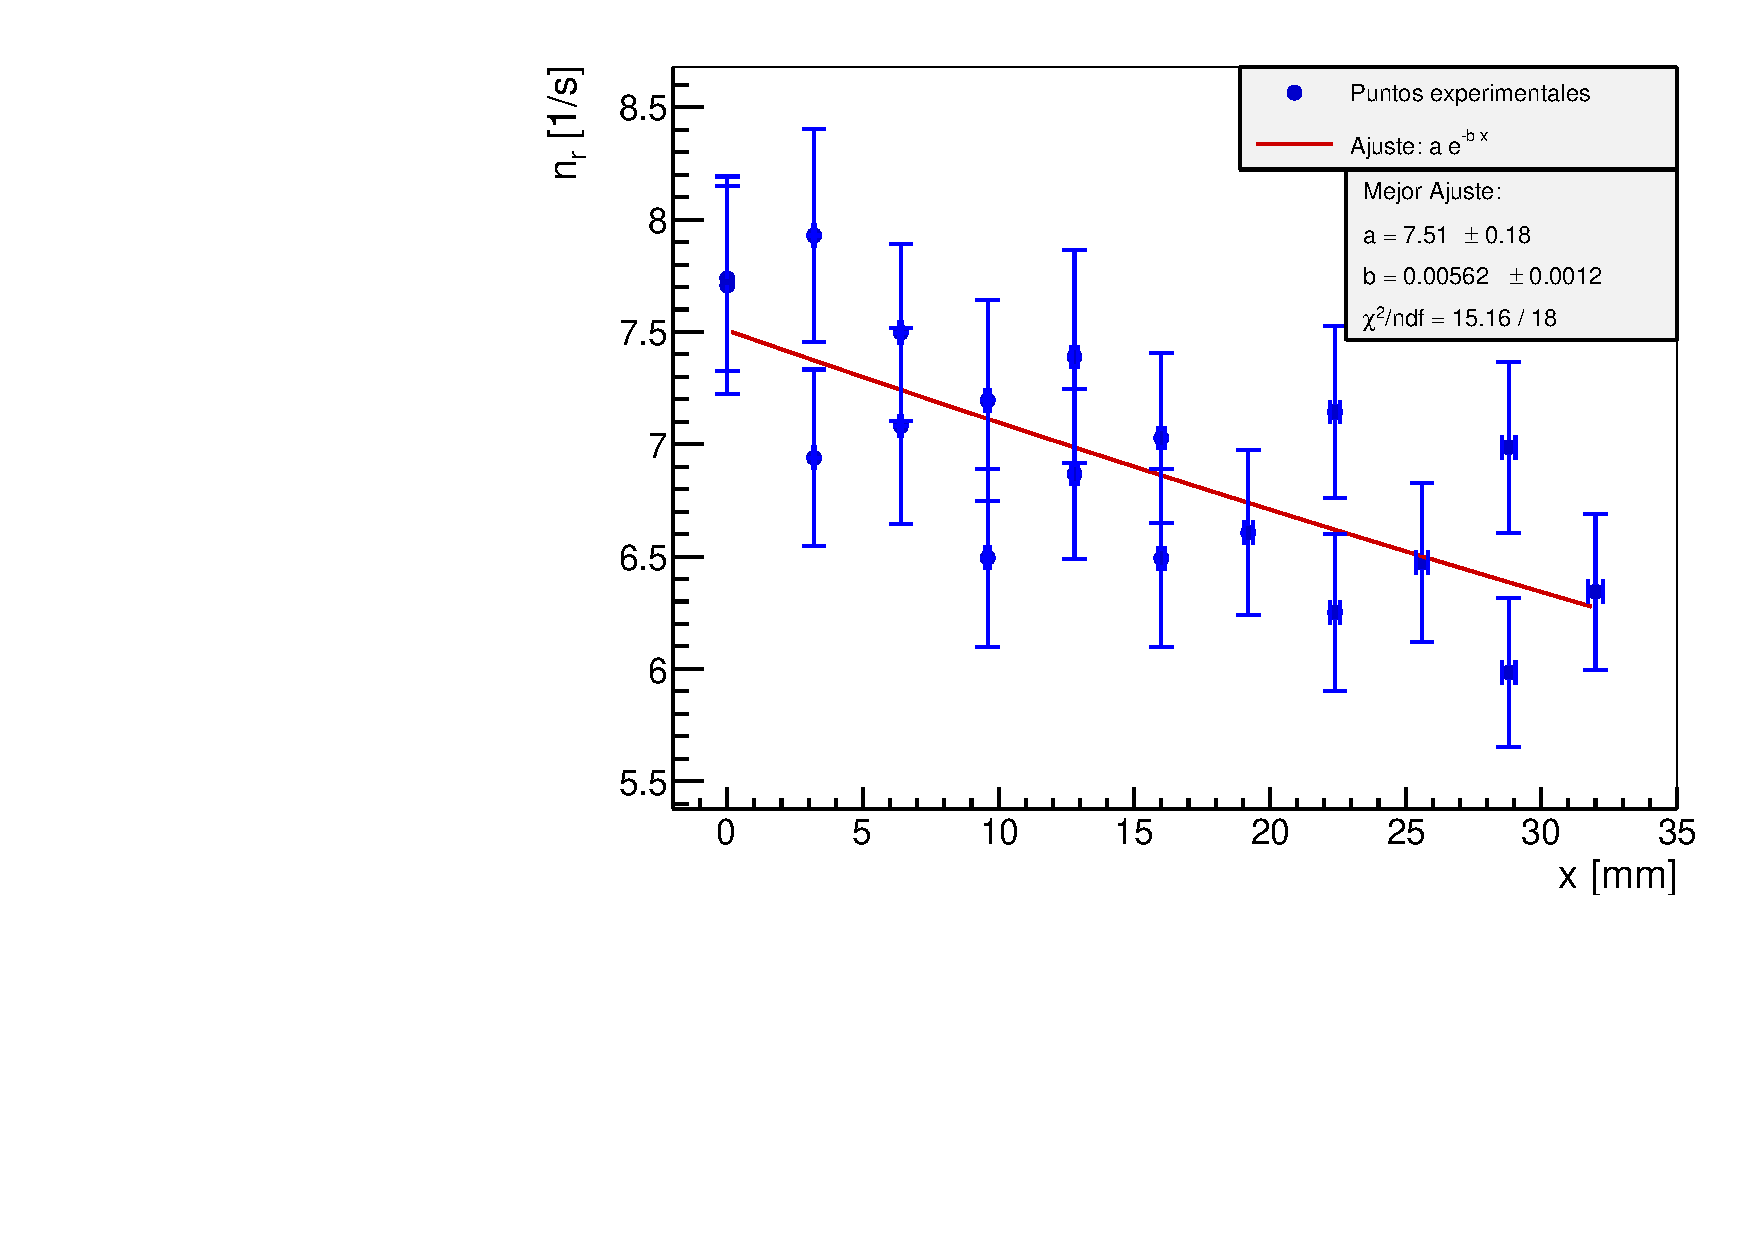
\includegraphics[width=1\linewidth]{../Graficas/Hierro.pdf}
\end{minipage}
\hfill
\begin{minipage}[t]{0.49\linewidth} \centering
	\captionof{figure}{Número de coincidencias reales en función del espesor de plomo.}
	\label{Fig:plomo}
	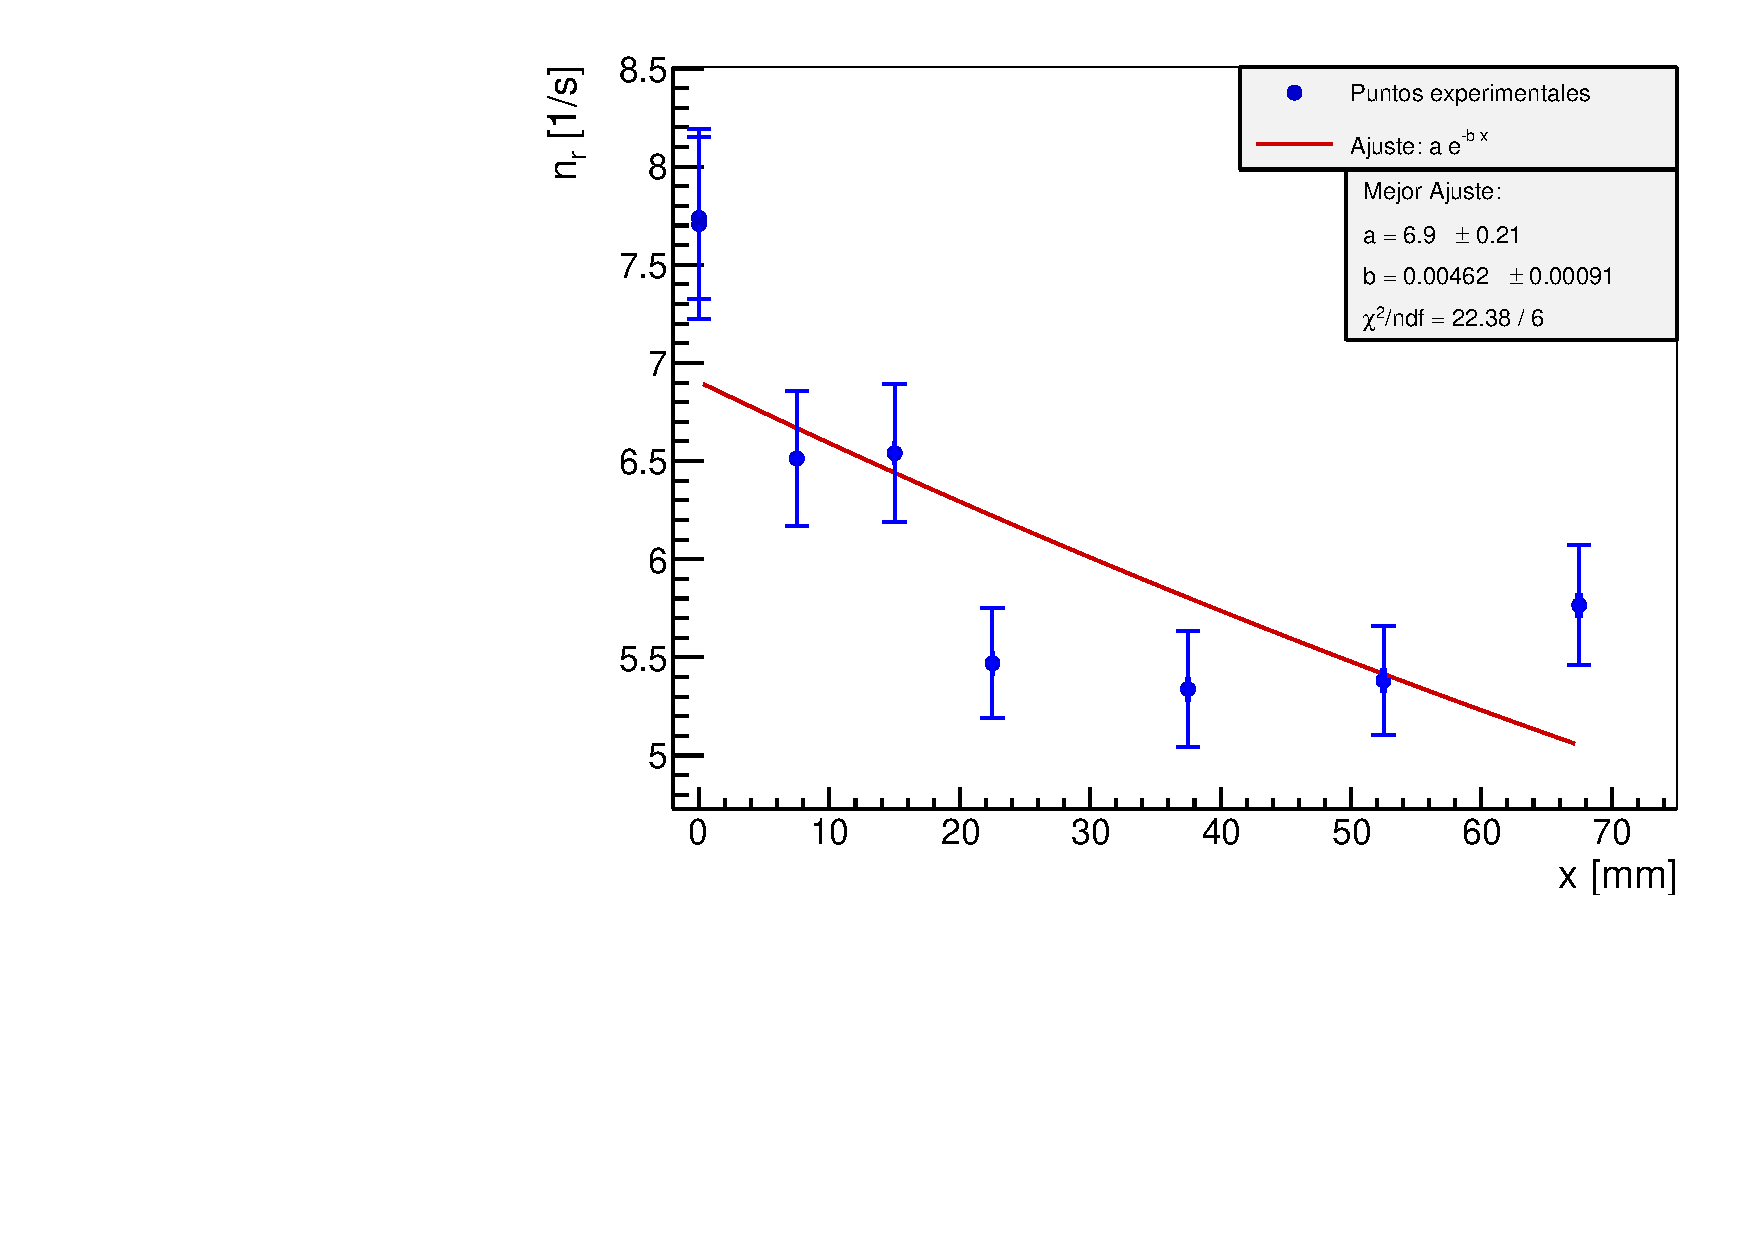
\includegraphics[width=1\linewidth]{../Graficas/Plomo2.pdf}
\end{minipage}

\begin{center}
\begin{table}[H]
\caption{Medidas de atenuación dura usando únicamente placas de plomo sin planchas de hierro}
\small
\label{Tab:plomo_2}
\begin{tabular}{cccccccccccccccccccccc}
\toprule
$x_{\text{Pb}}$ (mm) & $N_1$  & $N_2$ & $N_{12}$ & $t$ [s] & $n_1$ [s$^{-1}$] & $n_2$  [s$^{-1}$] & $n_{acc}$ [s$^{-1}$] & $n_{r}$ [s$^{-1}$] \\
\midrule
\num{0.0(0.0)} & \num{10326.0000000000(101.6169277237)} & \num{3988.0000000000(63.1506136154)} & \num{313.0000000000(17.6918060130)} & \num{36.6000000000(0.1300000000)} & \num{282.1311475410(2.9517310291)} & \num{108.9617486339(1.7682995938)} & \num{0.8447765074(0.0193277084)} & \num{7.7071360609(0.4847216248)} \\
\num{0.0(0.0)} & \num{17115.0000000000(130.8243096676)} & \num{6221.0000000000(78.8733161468)} & \num{462.0000000000(21.4941852602)} & \num{52.5000000000(0.1300000000)} & \num{326.0000000000(2.6193810628)} & \num{118.4952380952(1.5307336676)} & \num{1.0615372206(0.0234526395)} & \num{7.7384627794(0.4106627555)} \\
\num{7.5000000000(0.0140000000)} & \num{17450.0000000000(132.0984481362)} & \num{5952.0000000000(77.1492060879)} & \num{448.0000000000(21.1660104885)} & \num{61.6800000000(0.1300000000)} & \num{282.9118028534(2.2231321958)} & \num{96.4980544747(1.2672254112)} & \num{0.7502160517(0.0165863226)} & \num{6.5130783711(0.3438999098)} \\
\num{15.0000000000(0.0280000000)} & \num{16334.0000000000(127.8045382606)} & \num{5467.0000000000(73.9391641825)} & \num{429.0000000000(20.7123151772)} & \num{59.2600000000(0.1300000000)} & \num{275.6328045899(2.2398351409)} & \num{92.2544718191(1.2640145202)} & \num{0.6987712999(0.0155260323)} & \num{6.5405132090(0.3502208765)} \\
\num{22.5000000000(0.0420000000)} & \num{19751.0000000000(140.5382510209)} & \num{6151.0000000000(78.4283112148)} & \num{466.0000000000(21.5870331449)} & \num{77.3000000000(0.1300000000)} & \num{255.5109961190(1.8681796595)} & \num{79.5730918499(1.0233839183)} & \num{0.5587178630(0.0123039893)} & \num{5.4697426804(0.2797177548)} \\
\num{37.5000000000(0.0700000000)} & \num{18875.0000000000(137.3863166403)} & \num{5947.0000000000(77.1167945392)} & \num{413.0000000000(20.3224014329)} & \num{69.0000000000(0.1300000000)} & \num{273.5507246377(2.0567268633)} & \num{86.1884057971(1.1293696820)} & \num{0.6478932357(0.0143022089)} & \num{5.3376140107(0.2950901671)} \\
\num{52.5000000000(0.0980000000)} & \num{21546.0000000000(146.7855578727)} & \num{6703.0000000000(81.8718510845)} & \num{471.0000000000(21.7025344142)} & \num{78.0700000000(0.1300000000)} & \num{275.9830920968(1.9355276044)} & \num{85.8588446266(1.0583986971)} & \num{0.6511547974(0.0142739850)} & \num{5.3818924679(0.2785355961)} \\
\num{67.5000000000(0.1260000000)} & \num{18783.0000000000(137.0510853660)} & \num{5993.0000000000(77.4144689318)} & \num{444.0000000000(21.0713075057)} & \num{69.2600000000(0.1300000000)} & \num{271.1954952353(2.0432147453)} & \num{86.5290210800(1.1294752541)} & \num{0.6448533943(0.0142311445)} & \num{5.7657732300(0.3048051343)} \\
\bottomrule
\end{tabular}
\end{table}
\end{center}


\subsection{Laminas de hierro y planchas de plomo}

\textcolor{blue}{En este caso estamos repitiendo el mismo proceso que el anterior pero con 20 placas de hierro y colocando las planchas de plomo justamente encima.} En la \cref{Fig:plomohierro} vemos los datos de la \cref{Tab:plomo_1} representados gráficamente con el ajuste exponencial comentado anteriormente hecho. Como podemos ver el ajuste tiene $\chi^2/$ndf$<1$ de tal modo que es un buen ajsute, y no es descartable por hipótesis nula. Por otra parte, de los parámetros obtenidos podemos extraer los siguientes datos: 

\begin{equation}
	n_r(0) = 6.02(14) \ \unit{cuentas/s}  \tquad \lambda^\mu_m = 667(219) \ \unit{g/cm^2}
\end{equation}
Este valor $n_r(0)$ sería la suma de las coincidencias procedente de la componente muónica, ya que podemos consdierar que hemos frenado la compoennte electrónica con las 20 planchas de hierro, por lo que ya podemos extraer información de estas. Por otro lado, el recorrido libre medio másico también correspondería a la componente muónica. 

\begin{center}
\begin{table}[H]
\caption{Medidas de atenuación dura usando únicamente placas de plomo con 20 de hierro}
\small
\label{Tab:plomo_1}
\begin{tabular}{cccccccccccccccccccccc}
\toprule
$x_{\text{Pb}}$ (mm) & $N_1$  & $N_2$ & $N_{12}$ & $t$ [s] & $n_1$ [s$^{-1}$] & $n_2$  [s$^{-1}$] & $n_{acc}$ [s$^{-1}$] & $n_{r}$ [s$^{-1}$] \\
\midrule
\num{0.0(0.0)} & \num{16089.0000000000(126.8424219258)} & \num{5557.0000000000(74.5452882482)} & \num{415.0000000000(20.3715487875)} & \num{58.8400000000(0.1300000000)} & \num{273.4364377974(2.2387687945)} & \num{94.4425560843(1.2839832053)} & \num{0.7096445124(0.0157600682)} & \num{6.3433806406(0.3469280454)} \\
\num{0.0(0.0)} & \num{16089.0000000000(126.8424219258)} & \num{5557.0000000000(74.5452882482)} & \num{415.0000000000(20.3715487875)} & \num{58.8400000000(0.1300000000)} & \num{273.4364377974(2.2387687945)} & \num{94.4425560843(1.2839832053)} & \num{0.7096445124(0.0157600682)} & \num{6.3433806406(0.3469280454)} \\
\num{7.5000000000(0.0140000000)} & \num{17091.0000000000(130.7325514170)} & \num{5418.0000000000(73.6070648783)} & \num{406.0000000000(20.1494416796)} & \num{62.2200000000(0.1300000000)} & \num{274.6865959499(2.1781062908)} & \num{87.0781099325(1.1969214170)} & \num{0.6572993302(0.0145973470)} & \num{5.8679337139(0.3244572681)} \\
\num{7.5000000000(0.0140000000)} & \num{16888.0000000000(129.9538379579)} & \num{5633.0000000000(75.0533143838)} & \num{412.0000000000(20.2977831302)} & \num{60.6600000000(0.1300000000)} & \num{278.4042202440(2.2238640690)} & \num{92.8618529509(1.2531814349)} & \num{0.7104440608(0.0157540322)} & \num{6.0815110991(0.3353023553)} \\
\num{15.0000000000(0.0280000000)} & \num{17940.0000000000(133.9402852020)} & \num{5424.0000000000(73.6478105581)} & \num{409.0000000000(20.2237484162)} & \num{65.3100000000(0.1300000000)} & \num{274.6899402848(2.1224749278)} & \num{83.0500689022(1.1397177916)} & \num{0.6269017475(0.0139089319)} & \num{5.6355389201(0.3102205260)} \\
\num{15.0000000000(0.0280000000)} & \num{18321.0000000000(135.3550885634)} & \num{6061.0000000000(77.8524244966)} & \num{415.0000000000(20.3715487875)} & \num{67.1300000000(0.1300000000)} & \num{272.9182183822(2.0844300167)} & \num{90.2875018621(1.1728324490)} & \num{0.6771375421(0.0149433283)} & \num{5.5048973157(0.3040676243)} \\
\num{15.0000000000(0.0280000000)} & \num{18008.0000000000(134.1938895777)} & \num{5570.0000000000(74.6324326282)} & \num{406.0000000000(20.1494416796)} & \num{64.8600000000(0.1300000000)} & \num{277.6441566451(2.1425093081)} & \num{85.8772741289(1.1634722706)} & \num{0.6552145257(0.0145188810)} & \num{5.6044216137(0.3112525815)} \\
\num{22.5000000000(0.0420000000)} & \num{16645.0000000000(129.0155029444)} & \num{5288.0000000000(72.7186358508)} & \num{414.0000000000(20.3469899494)} & \num{62.5000000000(0.1300000000)} & \num{266.3200000000(2.1372823229)} & \num{84.6080000000(1.1767321673)} & \num{0.6192014143(0.0137722560)} & \num{6.0047985857(0.3261341842)} \\
\num{37.5000000000(0.0700000000)} & \num{17336.0000000000(131.6662447251)} & \num{5496.0000000000(74.1350119714)} & \num{408.0000000000(20.1990098767)} & \num{66.0000000000(0.1300000000)} & \num{262.6666666667(2.0609399710)} & \num{83.2727272727(1.1351701274)} & \num{0.6010692073(0.0133336302)} & \num{5.5807489745(0.3065778205)} \\
\num{45.0000000000(0.0840000000)} & \num{17645.0000000000(132.8344834747)} & \num{5710.0000000000(75.5645419493)} & \num{405.0000000000(20.1246117975)} & \num{66.6600000000(0.1300000000)} & \num{264.7014701470(2.0584950096)} & \num{85.6585658566(1.1458241552)} & \num{0.6230800996(0.0137938480)} & \num{5.4525274611(0.3024465040)} \\
\num{52.5000000000(0.0980000000)} & \num{18037.0000000000(134.3018987208)} & \num{5662.0000000000(75.2462623656)} & \num{419.0000000000(20.4694894905)} & \num{67.5700000000(0.1300000000)} & \num{266.9379902324(2.0528746652)} & \num{83.7945833950(1.1252135167)} & \num{0.6146714772(0.0136078684)} & \num{5.5863052877(0.3034776059)} \\
\num{60.0000000000(0.1120000000)} & \num{18094.0000000000(134.5139397981)} & \num{5698.0000000000(75.4850978671)} & \num{410.0000000000(20.2484567313)} & \num{67.7400000000(0.1300000000)} & \num{267.1095364629(2.0508358765)} & \num{84.1157366401(1.1259673869)} & \num{0.6174238118(0.0136641717)} & \num{5.4351300707(0.2994518418)} \\
\num{67.5000000000(0.1260000000)} & \num{17038.0000000000(130.5296901092)} & \num{5252.0000000000(72.4706837280)} & \num{404.0000000000(20.0997512422)} & \num{63.4900000000(0.1300000000)} & \num{268.3572216097(2.1280721505)} & \num{82.7216884549(1.1539488288)} & \num{0.6100274890(0.0135669850)} & \num{5.7531793153(0.3171396927)} \\
\num{67.5000000000(0.1260000000)} & \num{18248.0000000000(135.0851583261)} & \num{5732.0000000000(75.7099729230)} & \num{416.0000000000(20.3960780544)} & \num{67.0600000000(0.1300000000)} & \num{272.1145243066(2.0823171813)} & \num{85.4756934089(1.1410835431)} & \num{0.6391622019(0.0141403620)} & \num{5.5642377385(0.3047126271)} \\
\num{75.0000000000(0.1400000000)} & \num{19374.0000000000(139.1905169184)} & \num{5953.0000000000(77.1556867638)} & \num{407.0000000000(20.1742410018)} & \num{72.1900000000(0.1300000000)} & \num{268.3751212079(1.9877605198)} & \num{82.4629450062(1.0790534669)} & \num{0.6081599586(0.0134177011)} & \num{5.0297400275(0.2799664040)} \\
\bottomrule
\end{tabular}
\end{table}
\end{center}

\begin{figure}[h!] \centering	
	\caption{Número de coincidencias reales en función del espesor de plomo y 20 láminas de hierro con ajuste exponencial.}
	\label{Fig:plomohierro}
	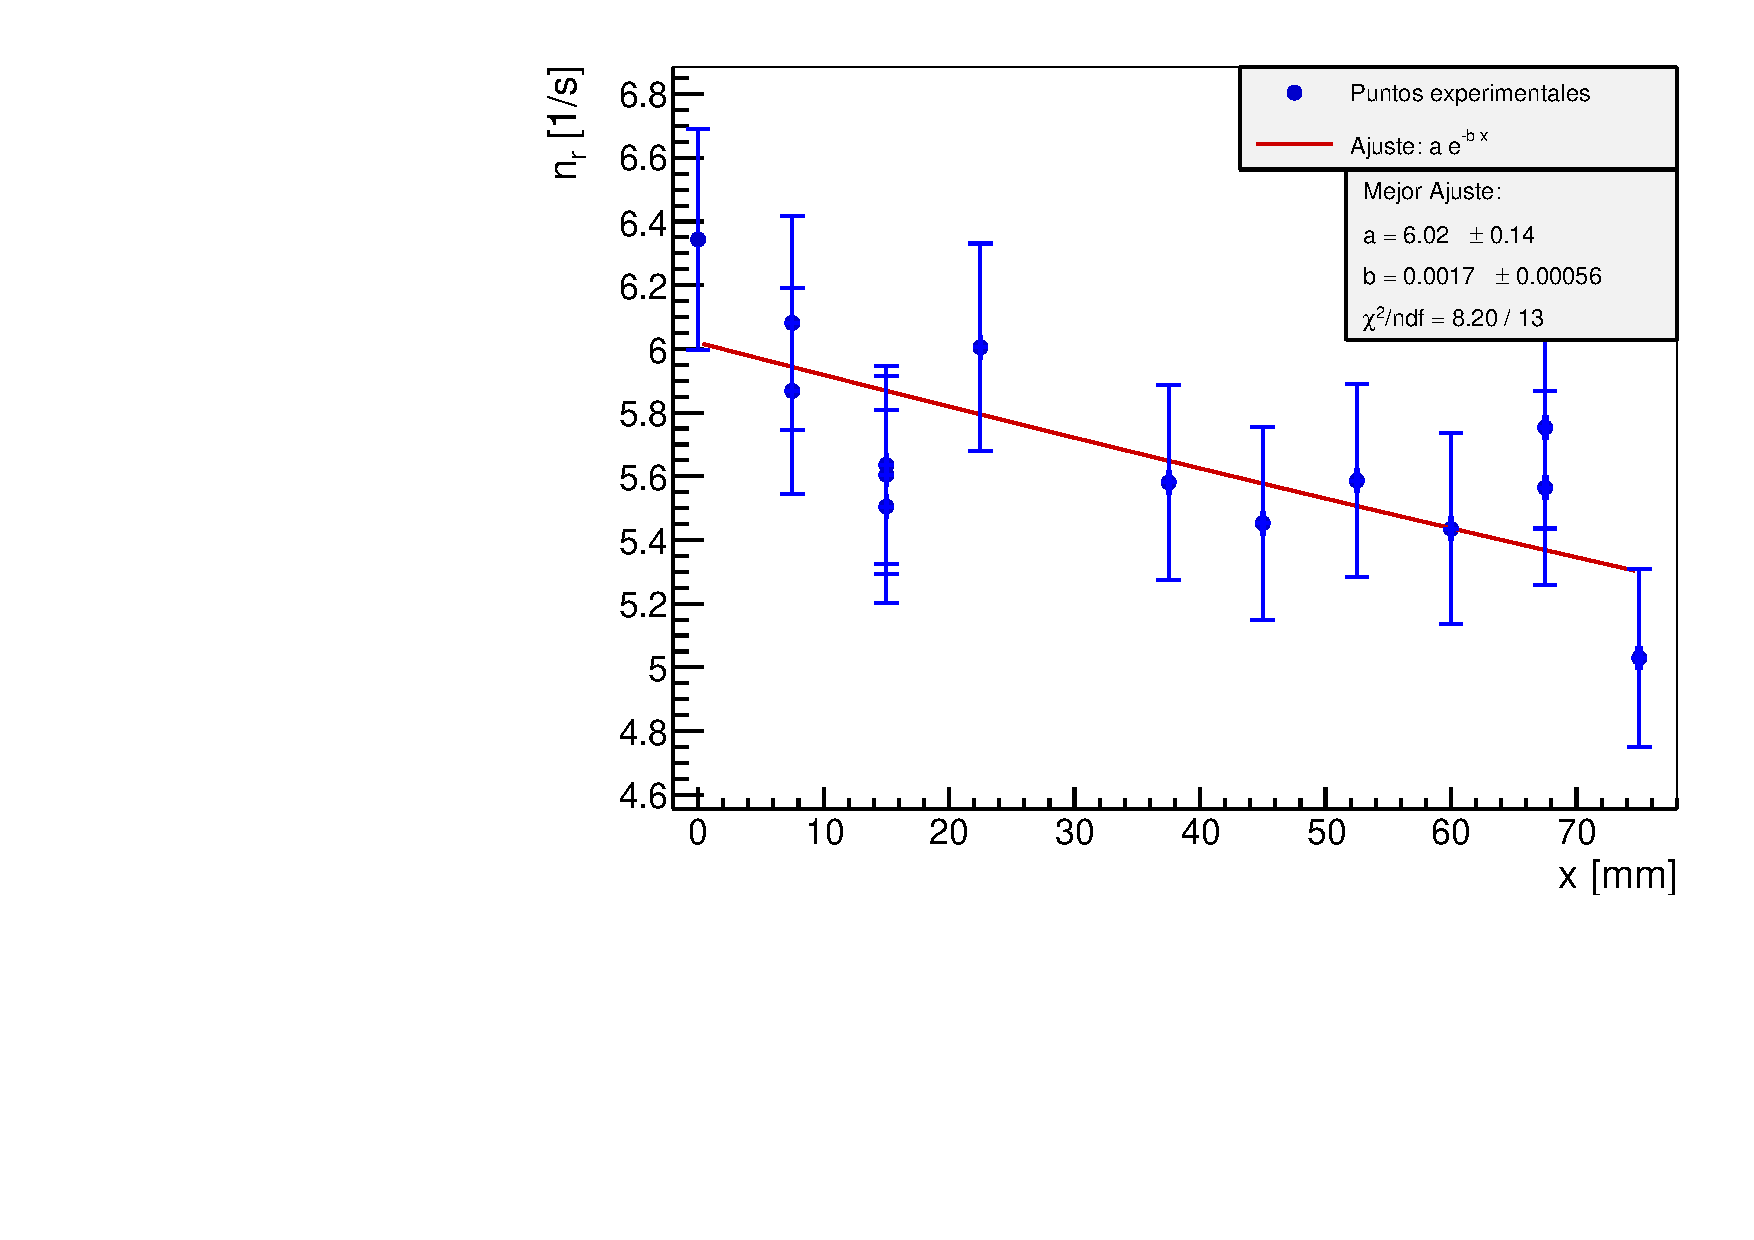
\includegraphics[width=0.72\linewidth]{../Graficas/Plomo.pdf}
\end{figure}

\subsection{Laminas de plomo, planchas de plomo y bloques de plomos}

En este apartado vamos a usar los datos de Celtia Jabares ya que nosotros no medimos datos sin bloques de plomo (de espesor 8.5 cm) ya que no se nos indico en la práctica que podíamos usarlos y nosotros considerabamos que eran importantes para parar la radiación de la fuente de alta radiación del cesio. Los datos de sus prácticas los hemos incluido en el anexo, \cref{Tab:hierroceltia} y \cref{Tab:plomoCeltia}. Por desgracia, para extraer los resultados de este apartado necesitamos sus valores de $n_r(0)$, ya que al tener diferentes voltajes umbrales y altos voltajes, medirse en días/horas diferentes, contar con diferentes sistemas de toma de datos, las fuentes de error que aparecerían por usar nuestro $n_r(0)$ serían muy elevadas. 

Como podemos ver $\chi^2$ de la \cref{Fig:hierroCeltia} es descartable para un 99\% de confianza $\chi^2_{0.95,5}=11.070$, por lo que sus datos no podemos extraer conclusiones de sus datos. Sin embargo, si podemos obtener datos de \cref{Fig:plomoCeltia}, ya que $\chi^2$ no es descartable $\chi^2_{0.90,3}=6.251$. Sin embargo, como hemos dicho, no podemos obtener un valor de $n_r$ para la componente muónica sin el valor de $n_r^\mu(0)$ dado por la atenuación de planchas de hierro o plomo. Lo que si podemos coger es un valor de $\lambda$ para los bloques de plomo, de tal modo que: 

\begin{equation}
	\lambda^\mu_m= 1163(155) \ \unit{g/cm^2}
\end{equation}
que como podemos ver es casi el doble del que obtuvimos nosotros en el apartado anterior. 

\begin{center}
\begin{table}[H]
\caption{Medidas de atenuación blanda usando únicamente placas de hierro,. Datos de Celtia Jabares.}
\small
\label{Tab:hierroceltia}
\begin{tabular}{cccccccccccccccccccccc}
\toprule
$x_{\text{Fe}}$ (mm) & $N_1$  & $N_2$ & $N_{12}$ & $t$ [s] & $n_1$ [s$^{-1}$] & $n_2$  [s$^{-1}$] & $n_{acc}$ [s$^{-1}$] & $n_{r}$ [s$^{-1}$] \\
\midrule
\num{4.8000000000(0.0420000000)} & \num{1200.0000000000(34.6410161514)} & \num{2700.0000000000(51.9615242271)} & \num{520.0000000000(22.8035085020)} & \num{180.0000000000(0.1300000000)} & \num{6.6666666667(0.1925103101)} & \num{15.0000000000(0.2888783385)} & \num{0.0027480000(0.0000743197)} & \num{2.8861408889(0.1267033598)} \\
\num{9.6000000000(0.0840000000)} & \num{1200.0000000000(34.6410161514)} & \num{2600.0000000000(50.9901951359)} & \num{456.0000000000(21.3541565041)} & \num{180.0000000000(0.1300000000)} & \num{6.6666666667(0.1925103101)} & \num{14.4444444444(0.2834708843)} & \num{0.0026462222(0.0000717411)} & \num{2.5306871111(0.1186483323)} \\
\num{14.4000000000(0.1260000000)} & \num{1100.0000000000(33.1662479036)} & \num{2700.0000000000(51.9615242271)} & \num{372.0000000000(19.2873015220)} & \num{180.0000000000(0.1300000000)} & \num{6.1111111111(0.1843097853)} & \num{15.0000000000(0.2888783385)} & \num{0.0025190000(0.0000690027)} & \num{2.0641476667(0.1071620925)} \\
\num{19.2000000000(0.1680000000)} & \num{1000.0000000000(31.6227766017)} & \num{2500.0000000000(50.0000000000)} & \num{398.0000000000(19.9499373433)} & \num{180.0000000000(0.1300000000)} & \num{5.5555555556(0.1757279046)} & \num{13.8888888889(0.2779588316)} & \num{0.0021203704(0.0000592379)} & \num{2.2089907407(0.1108445049)} \\
\num{24.0000000000(0.2100000000)} & \num{1000.0000000000(31.6227766017)} & \num{2500.0000000000(50.0000000000)} & \num{369.0000000000(19.2093727123)} & \num{180.0000000000(0.1300000000)} & \num{5.5555555556(0.1757279046)} & \num{13.8888888889(0.2779588316)} & \num{0.0021203704(0.0000592379)} & \num{2.0478796296(0.1067290234)} \\
\num{28.8000000000(0.2520000000)} & \num{1000.0000000000(31.6227766017)} & \num{2500.0000000000(50.0000000000)} & \num{280.0000000000(16.7332005307)} & \num{180.0000000000(0.1300000000)} & \num{5.5555555556(0.1757279046)} & \num{13.8888888889(0.2779588316)} & \num{0.0021203704(0.0000592379)} & \num{1.5534351852(0.0929690323)} \\
\num{32.0000000000(0.2800000000)} & \num{1000.0000000000(31.6227766017)} & \num{2400.0000000000(48.9897948557)} & \num{248.0000000000(15.7480157480)} & \num{180.0000000000(0.1300000000)} & \num{5.5555555556(0.1757279046)} & \num{13.3333333333(0.2723358292)} & \num{0.0020355556(0.0000570200)} & \num{1.3757422222(0.0874946535)} \\
\bottomrule
\end{tabular}
\end{table}
\end{center}

\begin{center}
\begin{table}[H]
\caption{Medidas de atenuación dura usando 20 láminas de hierro, 10 planchas de plomo y bloques de plomo. Datos de Celtia Jabares.}
\label{Tab:plomoCeltia}
\small
\begin{tabular}{cccccccccccccccccccccc}
\toprule
$x_{\text{Pb}}$ (mm) & $N_1$  & $N_2$ & $N_{12}$ & $t$ [s] & $n_1$ [s$^{-1}$] & $n_2$  [s$^{-1}$] & $n_{acc}$ [s$^{-1}$] & $n_{r}$ [s$^{-1}$] \\
\midrule
\num{170.0000000000(0.0280000000)} & \num{1900.0000000000(43.5889894354)} & \num{4900.0000000000(70.0000000000)} & \num{270.0000000000(16.4316767252)} & \num{300.0000000000(0.1300000000)} & \num{6.3333333333(0.1453225484)} & \num{16.3333333333(0.2334406549)} & \num{0.0028426533(0.0000703773)} & \num{0.8971573467(0.0547736894)} \\
\num{340.0000000000(0.0560000000)} & \num{2000.0000000000(44.7213595500)} & \num{5000.0000000000(70.7106781187)} & \num{262.0000000000(16.1864140562)} & \num{300.0000000000(0.1300000000)} & \num{6.6666666667(0.1490991881)} & \num{16.6666666667(0.2358128836)} & \num{0.0030533333(0.0000751231)} & \num{0.8702800000(0.0539560930)} \\
\num{510.0000000000(0.0840000000)} & \num{1800.0000000000(42.4264068712)} & \num{4900.0000000000(70.0000000000)} & \num{200.0000000000(14.1421356237)} & \num{300.0000000000(0.1300000000)} & \num{6.0000000000(0.1414452544)} & \num{16.3333333333(0.2334406549)} & \num{0.0026930400(0.0000670696)} & \num{0.6639736267(0.0471413850)} \\
\num{680.0000000000(0.1120000000)} & \num{2000.0000000000(44.7213595500)} & \num{5000.0000000000(70.7106781187)} & \num{153.0000000000(12.3693168769)} & \num{300.0000000000(0.1300000000)} & \num{6.6666666667(0.1490991881)} & \num{16.6666666667(0.2358128836)} & \num{0.0030533333(0.0000751231)} & \num{0.5069466667(0.0412317170)} \\
\num{850.0000000000(0.1400000000)} & \num{1900.0000000000(43.5889894354)} & \num{5000.0000000000(70.7106781187)} & \num{156.0000000000(12.4899959968)} & \num{300.0000000000(0.1300000000)} & \num{6.3333333333(0.1453225484)} & \num{16.6666666667(0.2358128836)} & \num{0.0029006667(0.0000717537)} & \num{0.5170993333(0.0416339916)} \\
\bottomrule
\end{tabular}
\end{table}
\end{center}


\begin{minipage}[t]{0.48\linewidth} \centering
	\captionof{figure}{Atenuación solo con láminas de hierro. Datos de Celtia Jabares \cref{Tab:hierroceltia}.}
	\label{Fig:hierroCeltia}
	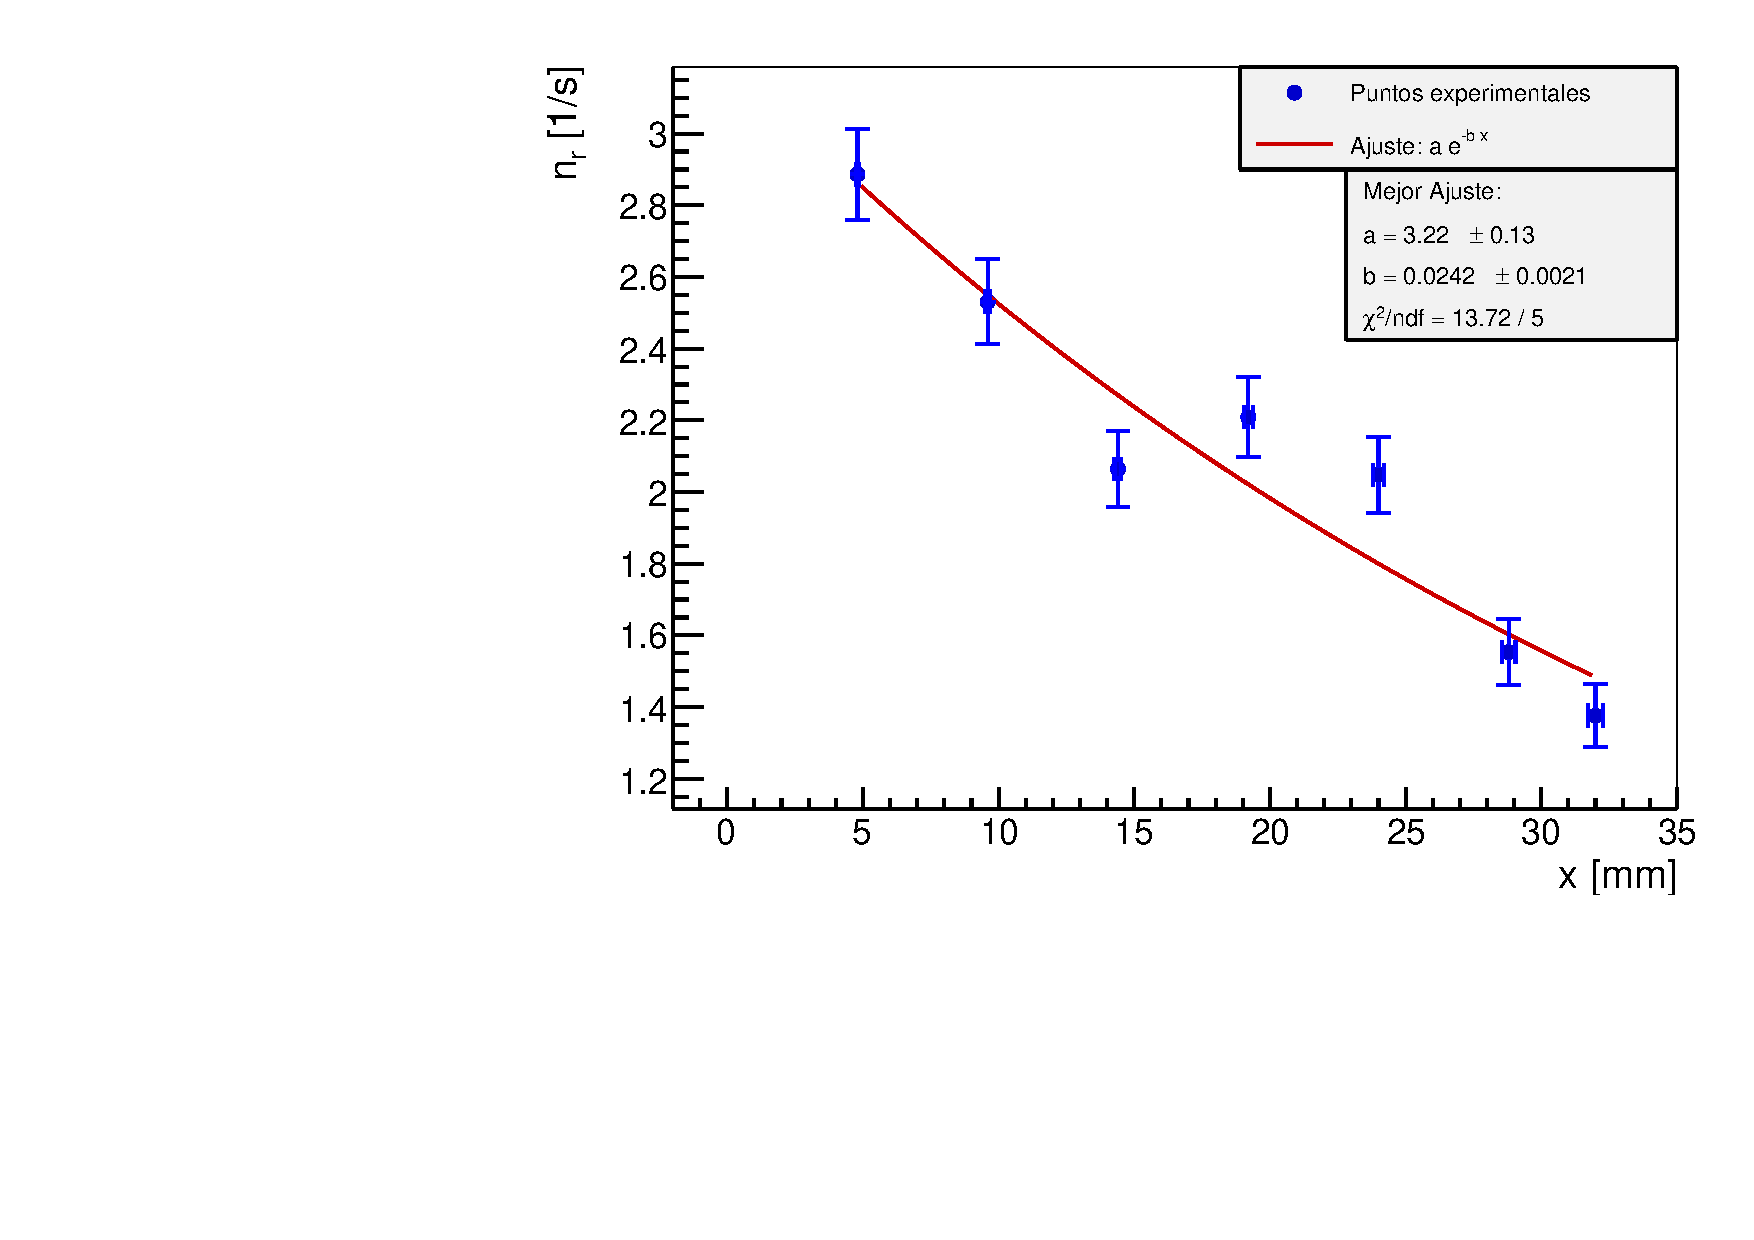
\includegraphics[width=1\linewidth]{../Graficas/HierroCeltia.pdf} 
\end{minipage}
\hfill
\begin{minipage}[t]{0.48\linewidth} \centering
	\captionof{figure}{Atenuación solo con bloques de plomo, 20 láminas de hierro y 10 planchas de plomo. Datos de Celtia Jabares \cref{Tab:plomoCeltia}.}
	\label{Fig:plomoCeltia}
	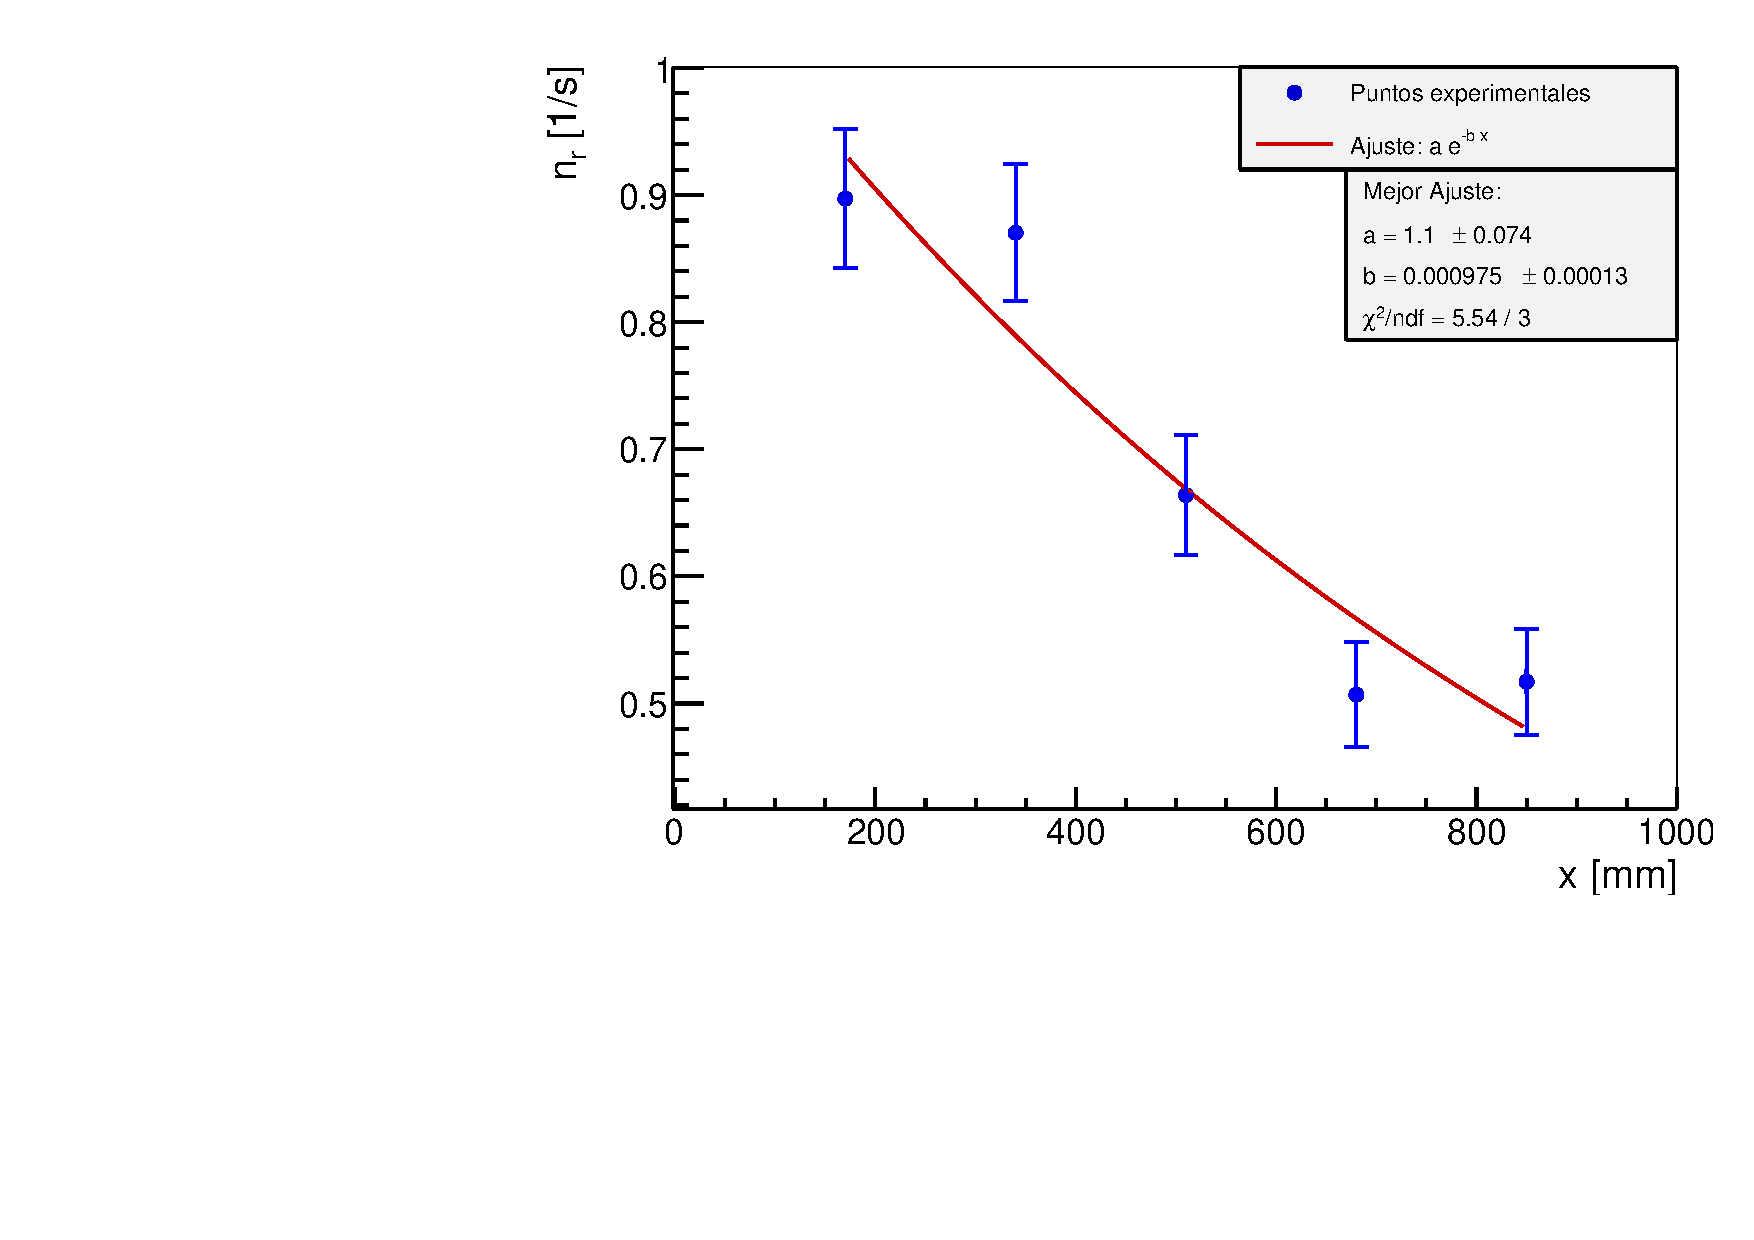
\includegraphics[width=1\linewidth]{../Graficas/PlomoCeltia.pdf}
\end{minipage}

\subsection{Conclusiones} \label{Subsec:6.5}

En este apartado vamos a extraer los resultados finales de los apartados anteriores. Como hemos dicho, los valores de $n_r^e(0)$ y $n_r^\mu(0)$ no los podemos extraer de los datos de Celtia, ya que el ajuste exponencial para el hierro no supera el test de chi cuadrado, por lo que estos los tendremos que obtener de nuestros resultados que si son aceptables. De los datos de Celtia lo único relevante que podemos extraer es \textbf{el recorrido libre medio másico muónico} ya que ella si tomo medidas de la atenuación con bloques de plomo, que como hemos podido ver tiene un valor: 

\begin{equation}
	\lambda_m^\mu = 1163(155) \ \unit{g/cm^2}
\end{equation}
el cual es similar al que nos dan teóricmente, al menos en orden. Lógicamente con 5 datos pocos resultados concluyentes podemos tomar. Por otro lado, los valores de la tasa de coincidencias los vamos a obtener usando nuestros datos, tal que: 

\begin{equation}
	n_r(0) = 7.51(18)  \ \unit{cuentas/s}  \tquad 
	n_r^\mu (0) = 6.02(14) \ \unit{cuentas/s} 
\end{equation}
con los que podemos extraer $n_r^e(0)$, que sería: 

\begin{equation}
	n_r^e(0) = 1.49(22)  \ \unit{cuentas/s}   
\end{equation}
donde hemos aplicado trivialmente que la componente electrónica es la diferencia de la total y la muónica: 

\begin{equation}
	n_r^e (0) = n_r (0) - n_r^\mu (0) \tquad u(n_r^e(0))=\sqrt{u(n_r (0) )^2 + u(n_r^\mu (0) )^2}
\end{equation}
 
\section{Flujo en la superficie}

En este apartado vamos a obtener el flujo de las componentes muónicas y electrónicas a partir de los valores anteriores y el área activa $A$. Aunque sea trivial, la ecuación para obtener el flujo $J$ y la incertidumbre del flujo a partir del area $A$ y la tasa de cuentas $n_r(0)$ es: 

\begin{equation}
	J = \frac{n_r(0)}{A} \qquad u(J) = \frac{u(n_r(0))}{A}
\end{equation}
El area activa que usamos es $300$ cm$^{-2}$ que es un valor ya dado para los centelleadores que teníamos. \textcolor{blue}{Dado que no tenemos acceso a él, ni información acerca del mismo, no podemos darle ningún tipo de incertidumbre de tipo A o B. Lo tomaremos como una cosntante universal sin incertidumbre}. Así obtenemos:

\begin{equation}
	J = 250.3(60)  \ \unit{m^{-2}s^{-1}} \qquad 
	J^\mu = 200.6(46) \ \unit{m^{-2}s^{-1}} \qquad 
	J^e = 49.7(73) \ \unit{m^{-2}s^{-1}}
\end{equation}
Los valores medidos en situaciones parecidas son de $ J \sim$ 180 $ \unit{m^{-2}s^{-1}}$, con flujos parciales de $J^\mu \sim$ 130 $ \unit{m^{-2}s^{-1}}$ para la componente muónica y $J^e \sim$ 50 $ \unit{m^{-2}s^{-1}}$ para la electromagnética, al menos eso según el guion \cite{P2}. Otros datos como Jeng-Wei Lin \cite{LIN201024} arrojan valores más parecidos a los nuestors con $J^\mu\sim 190 \ \unit{m^{-2}s^{-1}}$ (en EEUU), siendo la componente electrónica entorno a $1/4$, compatible con nuestros datos. Los resultados que obtuvimos está claro que no son muy \textcolor{blue}{compatibles con los} dados por el guión, ya que aunque la componente electrónica casa bastante, la componente total y muónica distan mucho (incluso sin hacer un test de chi cuadrado podemos ver que no son compatibles). \textcolor{blue}{Con esto no queremos decir que nuestros datos sean ``buenos o malos'', ni que sean mas o menos creibles, directamente no los juzgamos. Simplemente explicitamos otros datos para hacer una comparación con los nuestros, y ver si se alejan mucho o si siguen una tendencia.} 


Para mejorar los resultados evidentemente tendríamos que tomar más datos, sobretodo para estudiar si existe alguna fuente de error desconocida. Con más control sobre la disposición geométrica podríamos reducir posibles errores, ya que recordemos que al estar tapadas con una lona negra, no nos percatamos de posibles fallos en el trascurso de las medidas, a pesar de que hiciéramos comprobaciones permanentes. Además medir flujos de electrones y muones en un laboratorio de físcia nuclear en el que hay presentes más fuentes y radiación de la que podría haber en una situación normal también puede afectar a nuestras medidas, aunque posibles errores y mejoras para tomar las medidas serán discutidas con mas desarrollo en la sección de conclusiones. En cualquier caso, parace que las láminas de hierro si pueden llegar a ser suficientes para parar la radiación electrónica, sin reducir significativamente las muónicas, al menos nuestros datos avalan esa conclusión.

\section{Dependencia con el ángulo}

En esta sección vamos a estudiar la dependencia de la radiación cósmica con el ángulo al que orientamos el detector respecto al suelo, i.e. $\theta=0$ significa que la perpendicular del detector y el suelo son paralelos. Cabe destacar que las medidas se realizaron a una distancia de $d=36.10(21)$ cm entre ellos, por razones que serán comentadas más adelante, primero vamos a explicar porqué es interseante estudiar esta $n_r(\theta)$. El punto es que uno esperaría que la mayor parte de la radiación cósmica lleguera efectivamente con $0^\circ$ y que para $\theta=90^\circ$ no llegara prácticamente radiación cósmica. Esto último se debería, en parte, a que los rayos cósmicos horizontales tendrían que atravesar una gran cantidad de atmósfera siendo atenuados mucho más que los verticales (fenómeno similar al que ocurre cuando hay un atardecer y la dispersión Rayleigh). También es cierto que existen coincidencias accidentales las cuales no tendrían por que dejar de verse si estuvieran a $90^\circ$. Sin embargo la parte mas intersante es que nos ayuda a entender como funciona el ángulo sólido/distancia. 


Ahora tratemos cómo medimos los ángulos, ya que es una cuestión interesante. Sea $\Delta \theta$ la diferencia entre el ángulo real de entrada de una partícula y el ángulo con el que la etiquetamos. Para poder afirmar que una partícula incide con un ángulo $\theta$ (definido como el ángulo entre la vertical del laboratorio y la trayectoria de la partícula), es necesario separar suficientemente los detectores. ¿Por qué? Porque la separación entre detectores define un ángulo de aceptación $\theta_a$, que puede interpretarse como la desviación angular máxima $\Delta \theta^{\max}$ compatible con una coincidencia.

\begin{equation}
	\tan (\theta_a) = \frac{l_{\max}}{d}
\end{equation}
\begin{minipage}[t]{0.64\linewidth}
donde $l_{\max}$ es el lado más largo del detector, y $d$ la distancia entre ellos. Cuanto mayor sea $d$, más estrecho será el cono de aceptación, lo que implica una mayor precisión angular, pero también una menor tasa de detección. \\[0.1em]

No obstante, esto no significa que la incertidumbre angular sea simplemente $u(\theta) = \theta_a^{\max}$, ya que la probabilidad de detección de una partícula con ángulo exactamente igual a $\theta_a$ es muy baja. Es decir, el ángulo de aceptación nos da el rango geométrico máximo de desviación posible entre la trayectoria real y el ángulo con el que clasificamos la partícula. Por ello, conviene minimizarlo aumentando la separación entre detectores. En la imagen  de la derecha hecha en tikz tratamos de reflejar este ángulo de aceptancia, en el que podemos ver que una partícula en el rango de $(-\theta_a+\theta,\theta+\theta_a)$ podría ser etiquetada como $\theta$. De hecho sería un estudio interesante calcular esta incertidumbre dada por la apertura. 
\end{minipage}
\hfill
\begin{minipage}[t]{0.3\linewidth}
\begin{center}
\hspace*{-0.75cm}
\begin{tikzpicture}[scale=1]
\begin{scope}[shift={(-2,0)}]
	\begin{scope}[rotate=-45]
	% Detectores

	\draw[fill=blue!20] (-1.2, 0) rectangle (1.2, 0.3);
	\draw[fill=blue!20] (-1.2, 4) rectangle (1.2, 4.3);
	\node[rotate=-45] at (0, -0.4) {\small Detector inferior};
	\node[rotate=-45] at (0, 4.7) {\small Detector superior};
	
	% Cono de aceptación
	\draw[dashed, thick, red] (-1.2, 4.3) -- (1.2, 0.3);
	\draw[dashed, thick, red] (1.2, 4.3) -- (-1.3, 0.3);

	
	% Arco para theta_a
	\draw[thick,red,fill=red] (0.85, 0.8) arc[start angle=135, delta angle=33, radius=1];
	% Distancia d
	\draw(1.6, 0.3) -- (1.6, 4);
	\node[rotate=45] at (1.9, 2.3) {\small Distancia $d$};
	
	% Lado l_max-
	\draw (-1.2, -0.6) -- (1.2, -0.6);
	\node[rotate=-45] at (0, -0.9) {\small Lado $l_{\max}$};
	
	% Etiqueta
	\draw[thick] (0.0,0.0) -- (0.0,4);  % eje y
	\filldraw[black] (0.0,4) -- (-0.1,3.85) -- (0.1,3.85) -- cycle;  % punta eje y

	\draw[thick,blue] (0.0, 1.0) arc[start angle=90, delta angle=45, radius=1];

	\end{scope}

		
	\draw[thick] (0.0,0) -- (0.0,4);  % eje y
	\node at (1.4, -0.3) {\textcolor{red}{$\theta_a$}};
	\node at (0.2, 0.6) {\textcolor{blue}{$\theta$}};


	% Flechitas manuales
	\filldraw[black] (0.0,4) -- (-0.1,3.85) -- (0.1,3.85) -- cycle;  % punta eje y
\end{scope}
\end{tikzpicture}
\end{center}
\end{minipage}

\subsection{Distribuciones angulares y contraste con los datos}

A la energía que llegan los muones $2$ GeV se considera una buena distribución angular una que vaya con el coseno cuadrado respecto el ángulo de incidencia:
\begin{equation}
	j (\theta) = j_0 \cos^2 (\theta)
\end{equation}
sin embargo otros (Jeng-Wei Lin, \cite{LIN201024}) apuntan a que el exponente podría ser un parámetro libre para $\theta\leq 70^\circ$:

\begin{equation}
	j (\theta) = j_0 \cos^n (\theta)	
\end{equation}
Nosotros consideraremos ambos, además de añadir un término constante que sería esta ``incidencia  cósmica horizontal'' (aunque también podría haber una gran parte de coincidencias accidentales). Así pues, nosotros estudiaremos dos ajustes:

\begin{equation}
	j_1 (\theta) = a_1 + b_1 \cos^2(\theta)	 \tquad 
	j_2 (\theta) = a_2 + b_2 |\cos(\theta)|^n
\end{equation}
donde trivialmente $a_{1,2}=j_{\text{horizontal}}$ y $b_{1,2}=j_0$. Ahora bien, hemos dicho que esta ecuación sirve para los muones, ¿también sirve para los electrones? Dado que la masa del muon es unas 200 veces superior, uno podría pensar que aparecen más términos angulares (al ser más relativista) .La distribución angular de la radiación cósmica secundaria en la superficie terrestre está dominada por los muones, cuya componente sigue aproximadamente una ley del tipo $|\cos(\theta)|^n$, con $n \approx 2$ para energías superiores a 1 GeV. Esta dependencia se debe al alargamiento efectivo del trayecto atmosférico con el ángulo cenital, y al hecho de que los muones, al ser más masivos y menos propensos a desviaciones o pérdidas por interacción, mantienen su dirección y energía incluso tras recorrer trayectos inclinados. Por ello, el modelo angular simple con un término $|\cos(\theta)|^n$ se ajusta muy bien a su comportamiento.

Sin embargo, los electrones secundarios (producidos por cascadas electromagnéticas iniciadas por fotones o interacciones hadrónicas) son mucho más ligeros, y por tanto más sensibles a la dispersión múltiple, pérdidas por radiación y absorción. Esto hace que su flujo angular sea más isotrópico y menos direccional. En consecuencia, la dependencia con $|\cos(\theta)|^n$ puede no ser una buena descripcion; tendiendo a mostrar una componente más horizontal y difusa. Por tanto, la expresión ajustada es adecuada para muones, pero no necesariamente para electrones, que requerirían modelos más complejos o una descripción experimental específica. A primer orden todo indica a pensar que es válida \cite{P2}. Luego comentaremos el posible contraste de esto con nuestros datos. 

\begin{center}
\begin{table}[H]
\scriptsize
\caption{Medidas de coincidencias a una distancia $33.3$ cm entre los detectores a diferentes ángulos. Factor de cobertura al ángulo de $k=3$.}
\label{Tab:angulo}
\begin{tabular}{cccccccccccccccccccccc}
\toprule
$\theta$ ($^\circ$) & $N_1$  & $N_2$ & $N_{12}$ & $t$ [s] & $n_1$ [s$^{-1}$] & $n_2$  [s$^{-1}$] & $n_{acc}$ [s$^{-1}$] & $n_{r}$ [s$^{-1}$] \\
\midrule
\num{0.00} & \num{44041.0000000000(209.8594767934)} & \num{18297.0000000000(135.2664038111)} & \num{324.0000000000(18.0000000000)} & \num{172.8000000000(0.1300000000)} & \num{254.8668981481(1.2295074061)} & \num{105.8854166667(0.7868344241)} & \num{0.7415941781(0.0157292873)} & \num{1.1334058219(0.1053569869)} \\
\num{10.0000000000(0.8400000000)} & \num{55792.0000000000(236.2033022631)} & \num{25452.0000000000(159.5368296037)} & \num{399.0000000000(19.9749843554)} & \num{227.8300000000(0.1300000000)} & \num{244.8843435895(1.0461263694)} & \num{111.7148751262(0.7031404583)} & \num{0.7517765118(0.0158536022)} & \num{0.9995292864(0.0891023711)} \\
\num{25.0000000000(0.8400000000)} & \num{51215.0000000000(226.3073131828)} & \num{22894.0000000000(151.3076336475)} & \num{331.0000000000(18.1934053987)} & \num{210.6000000000(0.1300000000)} & \num{243.1861348528(1.0850181877)} & \num{108.7084520418(0.7215867426)} & \num{0.7264719499(0.0153462314)} & \num{0.8452279552(0.0877462853)} \\
\num{45.0000000000(0.8400000000)} & \num{65255.0000000000(255.4505823051)} & \num{27374.0000000000(165.4508990607)} & \num{316.0000000000(17.7763888346)} & \num{259.8700000000(0.1300000000)} & \num{251.1063223920(0.9909874155)} & \num{105.3372840266(0.6388449225)} & \num{0.7268695779(0.0153046083)} & \num{0.4891230338(0.0700987542)} \\
\num{60.0000000000(0.8400000000)} & \num{52123.0000000000(228.3046210658)} & \num{23612.0000000000(153.6619666671)} & \num{303.0000000000(17.4068951855)} & \num{219.3800000000(0.1300000000)} & \num{237.5923055885(1.0501617100)} & \num{107.6305953141(0.7033352378)} & \num{0.7027240915(0.0148373861)} & \num{0.6784410101(0.0807253596)} \\
\num{67.0000000000(0.8400000000)} & \num{56803.0000000000(238.3337995333)} & \num{27445.0000000000(165.6653252796)} & \num{315.0000000000(17.7482393493)} & \num{218.2500000000(0.1300000000)} & \num{260.2657502864(1.1029711076)} & \num{125.7502863688(0.7627488804)} & \num{0.8993789775(0.0189496636)} & \num{0.5439199916(0.0835037875)} \\
\num{77.0000000000(0.8400000000)} & \num{68655.0000000000(262.0209915255)} & \num{29397.0000000000(171.4555335940)} & \num{301.0000000000(17.3493515729)} & \num{267.5000000000(0.1300000000)} & \num{256.6542056075(0.9874271286)} & \num{109.8953271028(0.6431764675)} & \num{0.7750760897(0.0163044246)} & \num{0.3501575552(0.0668776062)} \\
\num{90.0000000000(0.8400000000)} & \num{72191.0000000000(268.6838290631)} & \num{30162.0000000000(173.6721048413)} & \num{292.0000000000(17.0880074906)} & \num{280.0100000000(0.1300000000)} & \num{257.8157922931(0.9669875466)} & \num{107.7175815149(0.6222482657)} & \num{0.7631551487(0.0160463202)} & \num{0.2796647506(0.0631026352)} \\
\bottomrule
\end{tabular}
\end{table}
\end{center}


En la \cref{Tab:angulo} mostramos los valroes obtenidos, mientras que en las figuras \cref{Fig:angulo1} y \cref{Fig:angulo2} mostramos las representaciones gráficas y los ajustes. En particualr en la primera represntamos todos los datos y en la segunda elminamos lso valores de 60$^\circ$ y 67$^\circ$, ya que consdieramos incluso en el mismo laboratorio que hubo algún tipo de error con la geometría puediendo hacer que las superficies activas dejaran de estar superpuestas. Como podemos ver para la primera imagen $\chi^2_{0.99,5}=15.086$ la primera regresión no es un buen ajuste, mientras que $\chi^2_{0.95,4}=9.488$ el ajuste es un poco mejor solo descartable con un 95\% probabilidad. Como podemos ver dista bastante del $n=2$ el mejor ajuste, lo que afianza nuestra creencia de que en dichos datos hubo un fallo en el trascurso de la medida que afecto a los datos. 

Para la figura \cref{Fig:angulo2} los valores de la $\chi^2$/ndf$<$1 para $n=4.63$, y el ajuste $n=2$ $\chi^2$/ndf$\sim$1 por lo que tanto el ajuste con $n=2$ como el que deja $n$ como parámetro libre son compatibles, por lo que podemos considerar que efectivamente las coincidencias obtenidas son compatibles con una distribución angular $j_1(\theta)$ y $j_2(\theta)$. Sin embargo está claro que $n=4.63$ ajusta mucho mejor nuestros datos que $n=2$, por lo que es probable que para el rango de energías de nuestros muones $n=4.63$ sea mejor ajuste.

\begin{minipage}[t]{0.47\linewidth}
	\captionof{figure}{Ajuste $a + b \cos^2(\theta)$ y $a + b \cos^n(\theta)$  a los valores experimentales.}
	\label{Fig:angulo1}
	\begin{center}
	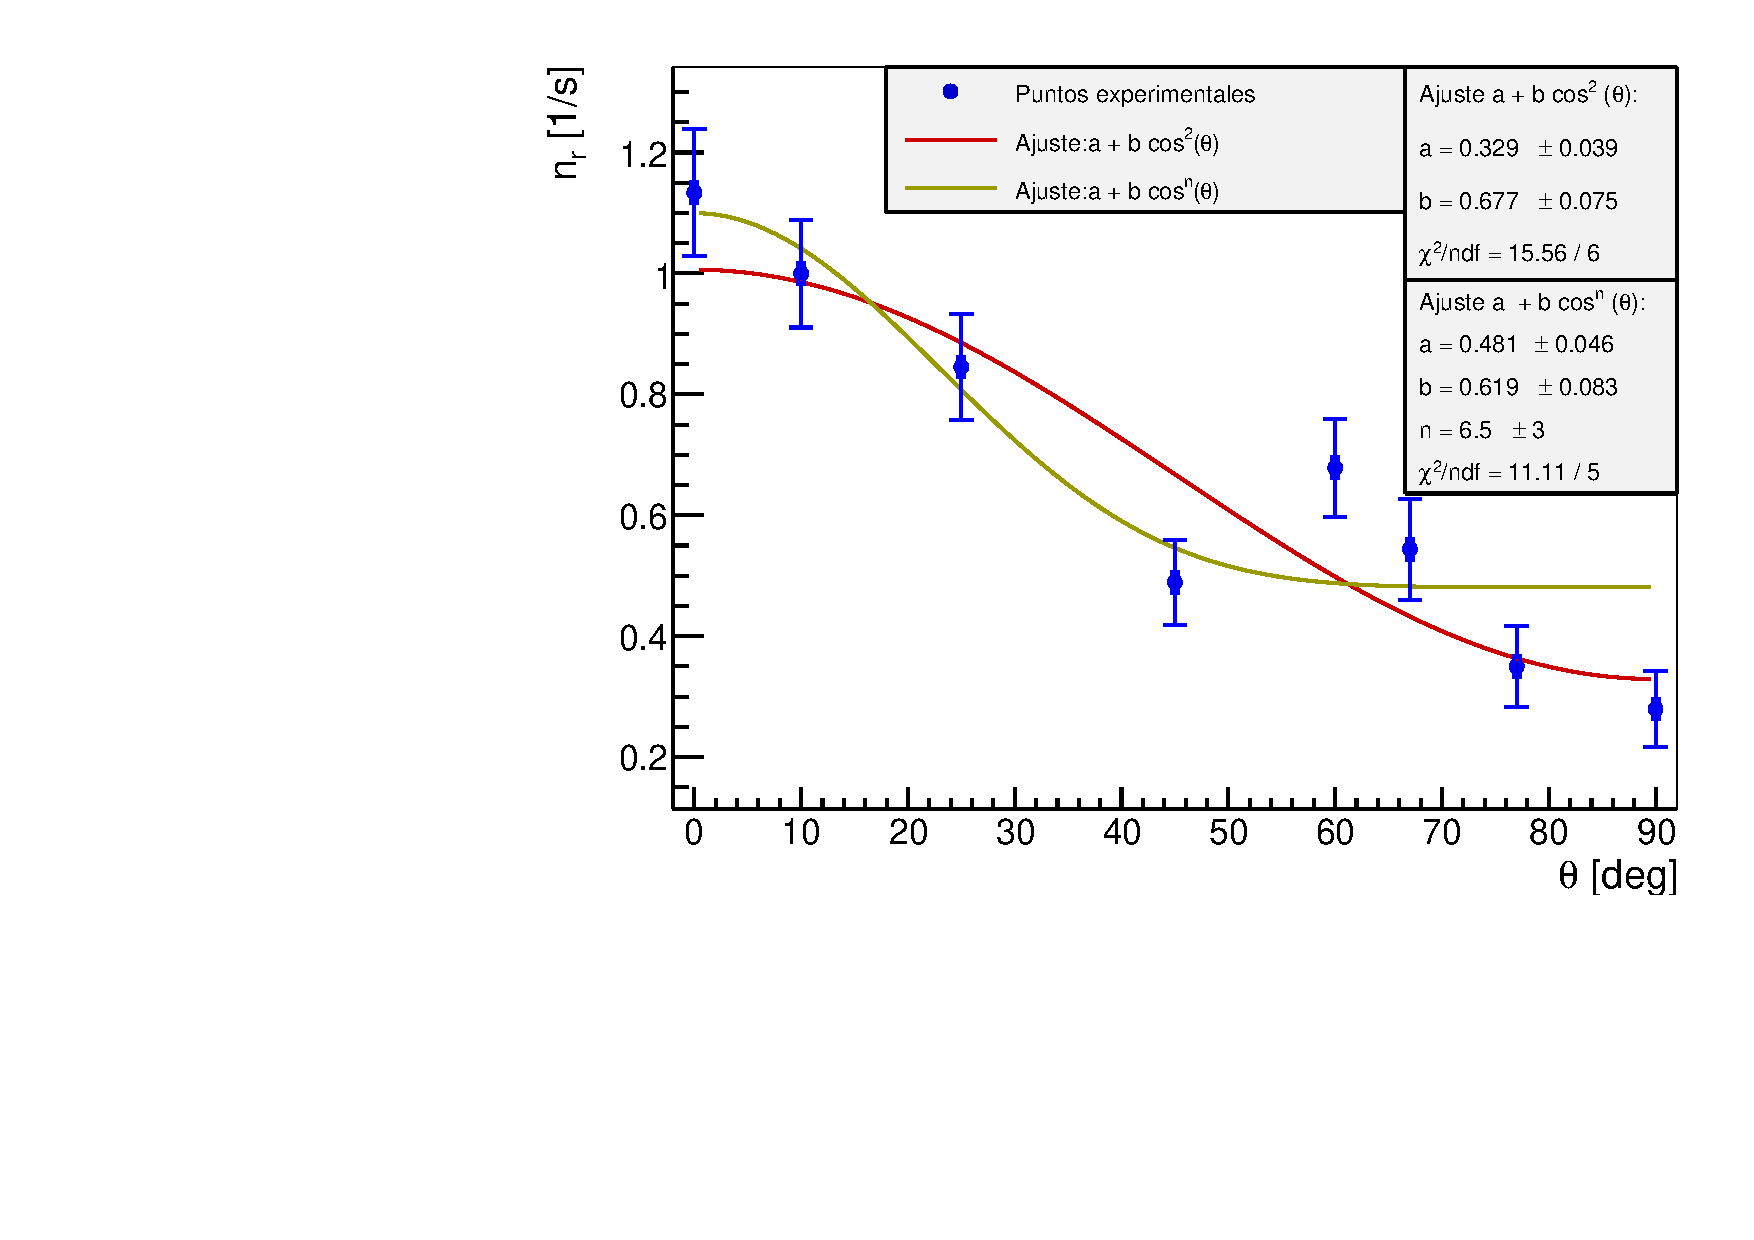
\includegraphics[width=0.99\linewidth]{../Graficas/Angulos.pdf}
	\end{center}
\end{minipage}
\hfill
\begin{minipage}[t]{0.47\linewidth}
	\captionof{figure}{Ajuste $a + b \cos^2(\theta)$ y $a + b \cos^n(\theta)$ a los valores experimentales eliminando 60$^\circ$ y 67$^\circ$.}
	\label{Fig:angulo2}
	\begin{center}
	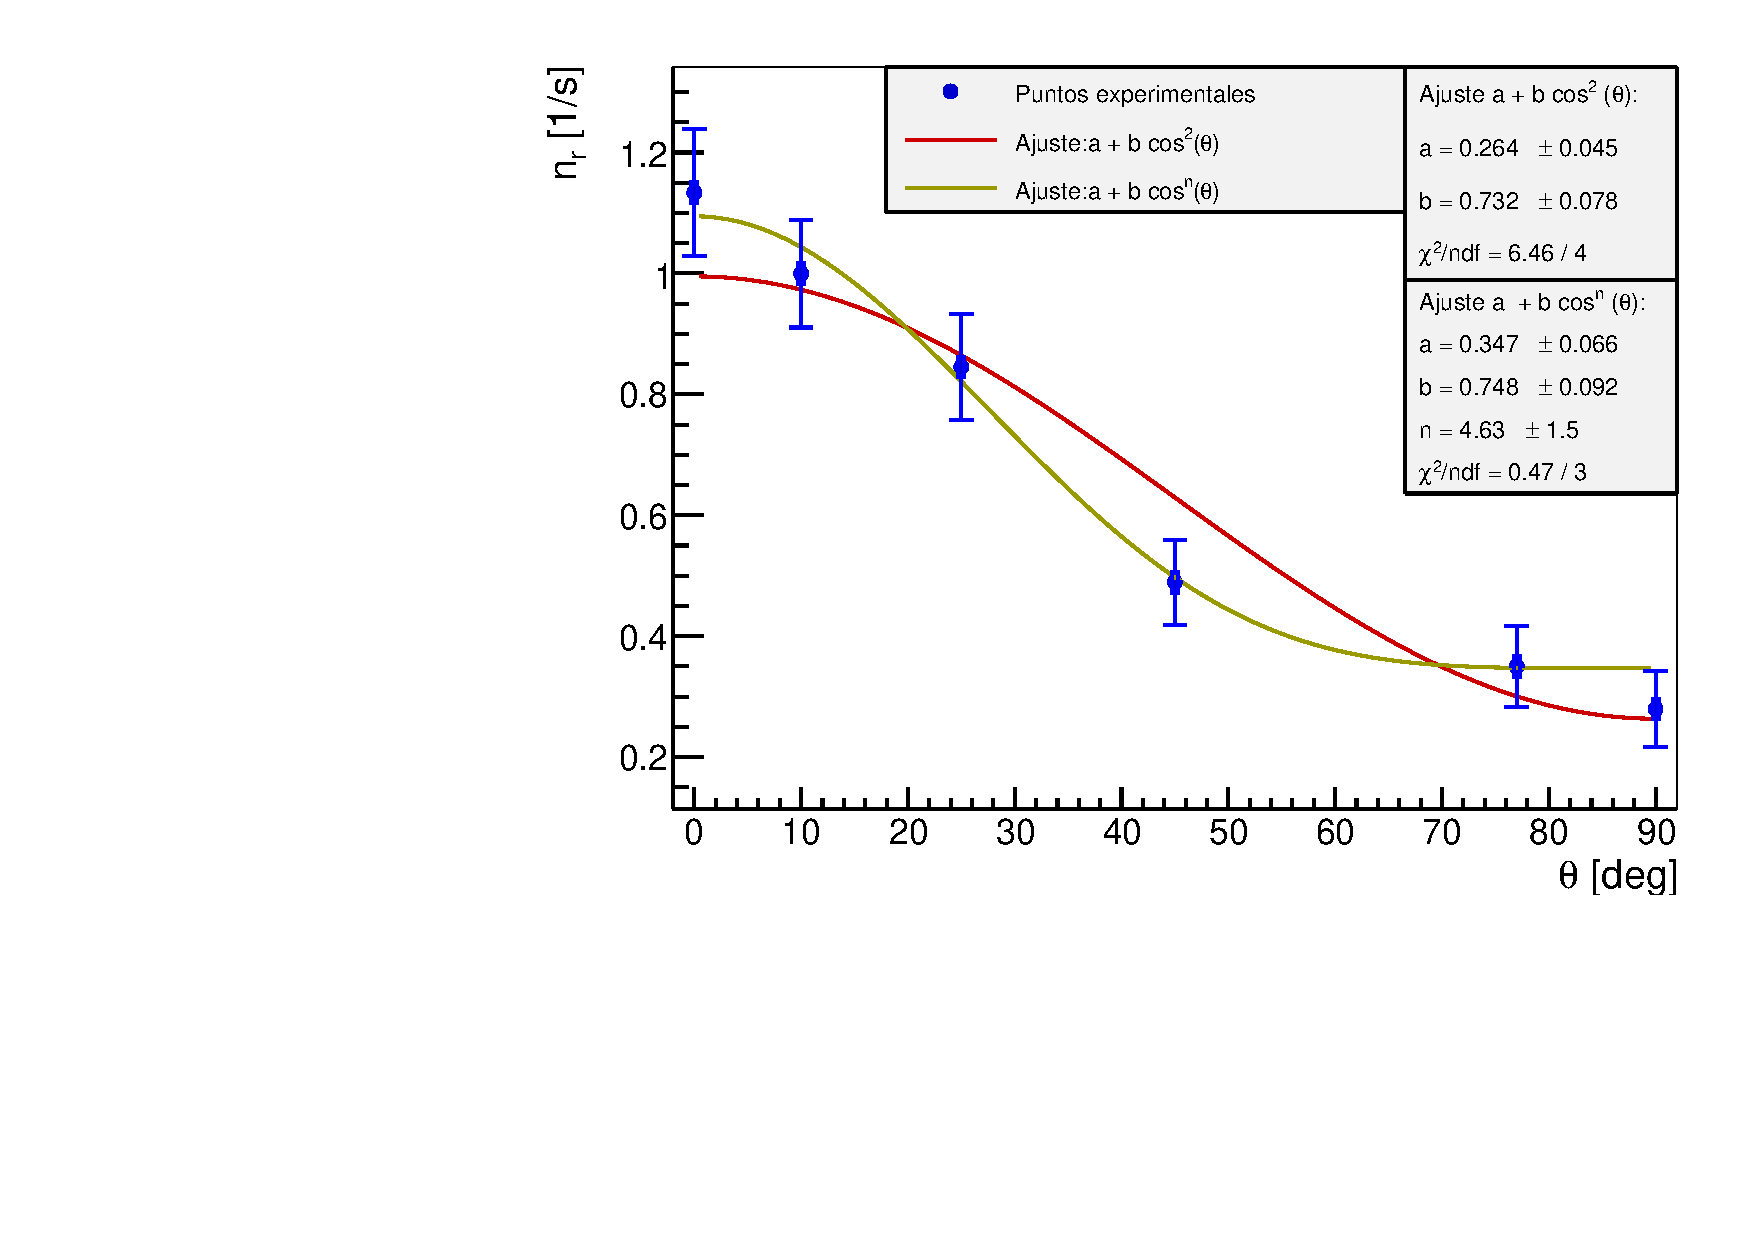
\includegraphics[width=0.99\linewidth]{../Graficas/Angulos_2.pdf}
	\end{center}
\end{minipage}


\subsection{¿Separación de componente muónica y electrónica?}

En el guion se nos pide que evaluemos con nuestros resultados si la componente blanda (electrónica) sigue realmente la misma distribución que la componente dura. Sin una atenuación es complicado comprobarlo, la única manera sería estudiando un comportamiento quizás como la suma de dos potencias del coseno:

\begin{equation}
	j(\theta)=a \cos^{n_1}(\theta)+ b \cos^{n_2}(\theta) + c
\end{equation}
pero ni siquiera así podríamos afirmar que no siguen la misma distribución, ya que en los datos no parece haber este comportamiento, y si se ajusta mejor también se deberá a la gran cantidad de parámetros libres. Francamente no nos parece que con los datos qeu tenemos podemos afirmar que no sigue la misma distribución, aunque tampoco podemos afirmar lo contrario. \textcolor{blue}{Sencillamente tenemos una falta de sensibilidad a una y otra distribución, que solo podría remediarse  obteniendo más datos y reduciendo la incertidumbre de los datos, ambas a la vez. Una vez ocurra esto, deberíamos ser capaces de diferenciar uno y otro comportamiento, y quizás inferir alguna conclusión estadísticamente plausible.}. El único indicio que nos parece hablar de ello es que en \cref{Fig:angulo2} es ajustable para 2 valores de $n$ diferentes, aunque no es concluyente estadísticamente. Otra manera sería suponer que efectivament $n_1=2$ tal que: 

\begin{equation}
	j_{3}(\theta)=a \cos^{2}(\theta)+ b \cos^{n_2}(\theta) + c
\end{equation}
o incluso con $b=a/4$ obteniendo igual que antes 3 parámetros libres (considerando que efectivamente la radiación electrónica incidente es un cuarto de la radiación muónica). Como podemos ver en \cref{Fig:angulo3} y \cref{Fig:angulo4}, el ajsute $j_3$ es compatible con nuestros datos, aunque no se ajusta mejor que $j_2(\theta)$, por lo que no podmos concluir ningún resultado sobre si la componente muónica y electrónica son diferentes.

\begin{minipage}[t]{0.47\linewidth}
	\captionof{figure}{Ajuste $j_1$ y $j_3$  a los valores experimentales.}
	\label{Fig:angulo3}
	\begin{center}
	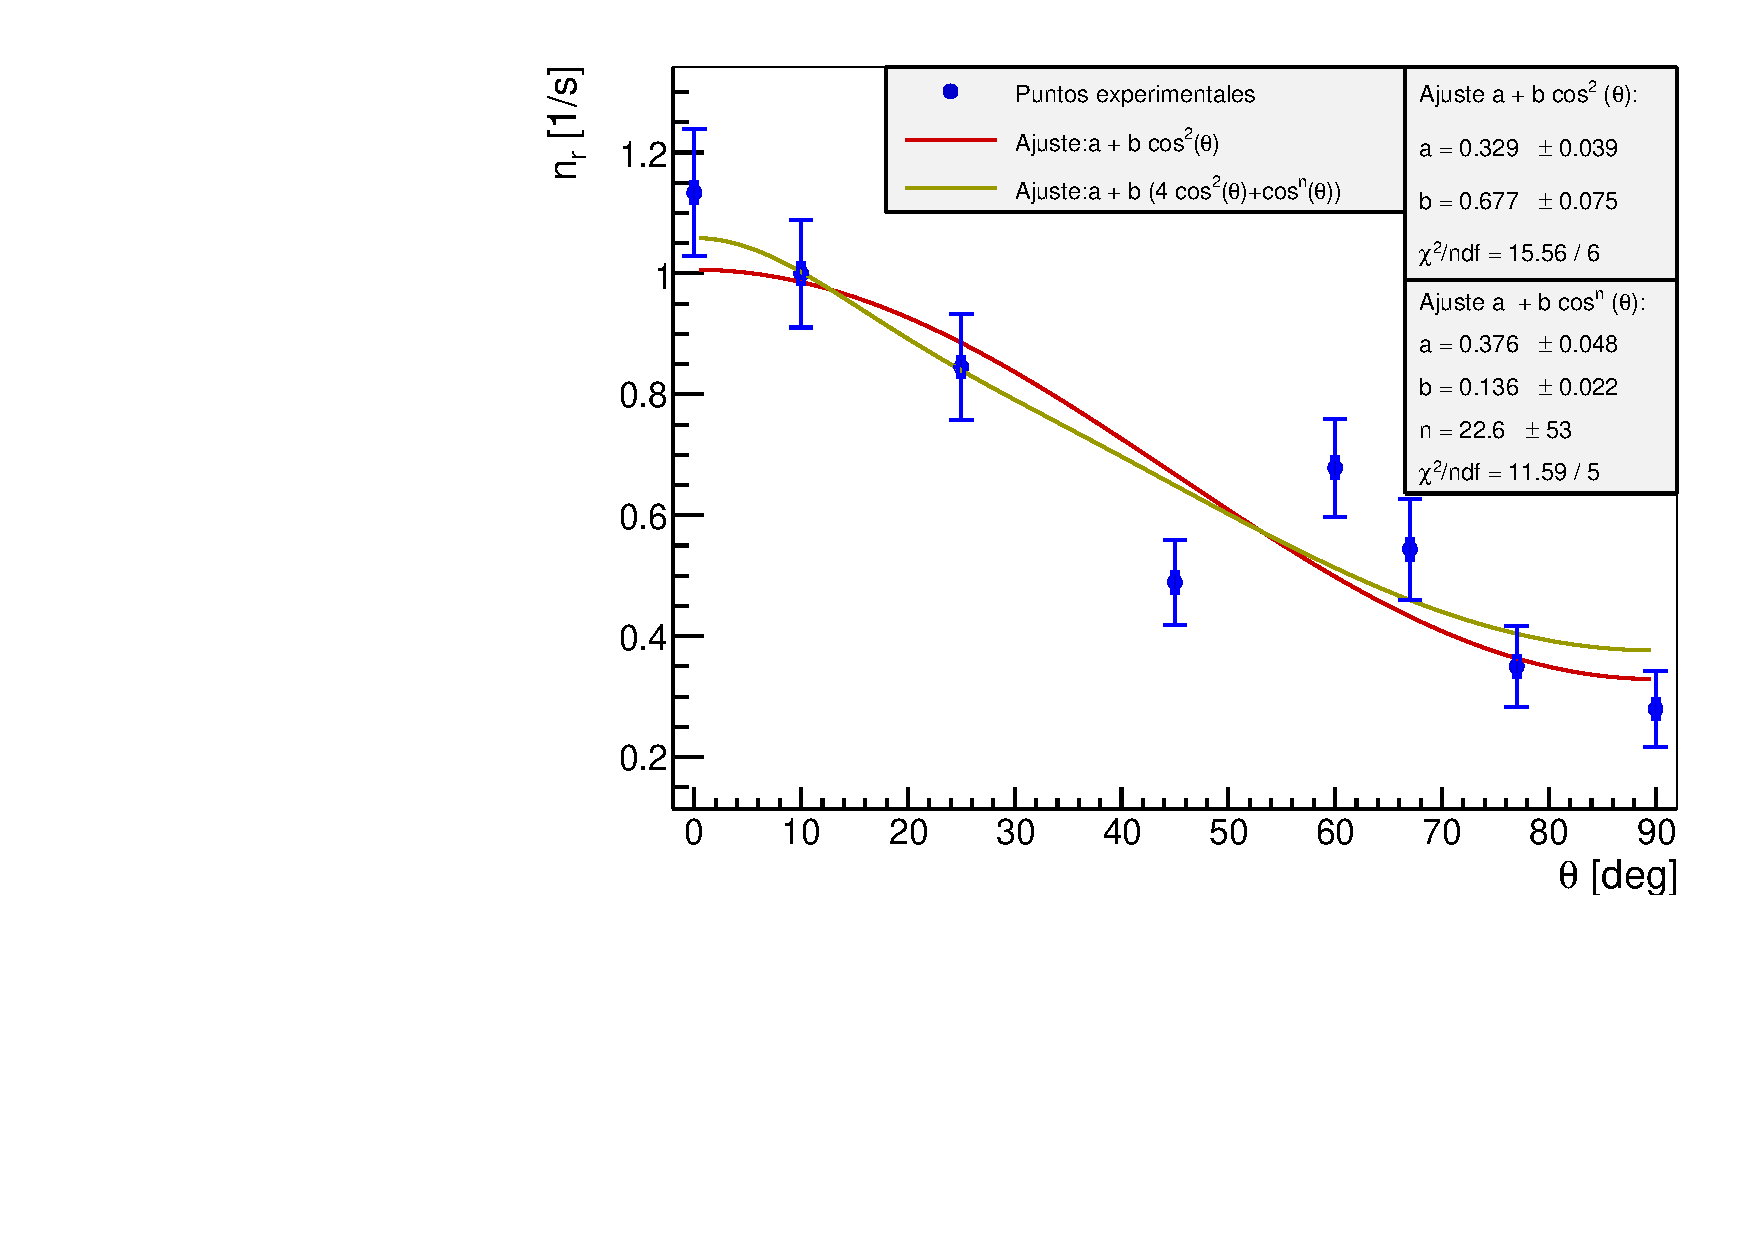
\includegraphics[width=0.99\linewidth]{../Graficas/Angulos_3.pdf}
	\end{center}
\end{minipage}
\hfill
\begin{minipage}[t]{0.47\linewidth}
	\captionof{figure}{Ajuste $j_1$ y $j_3$ a los valores experimentales eliminando 60$^\circ$ y 67$^\circ$.}
	\label{Fig:angulo4}
	\begin{center}
	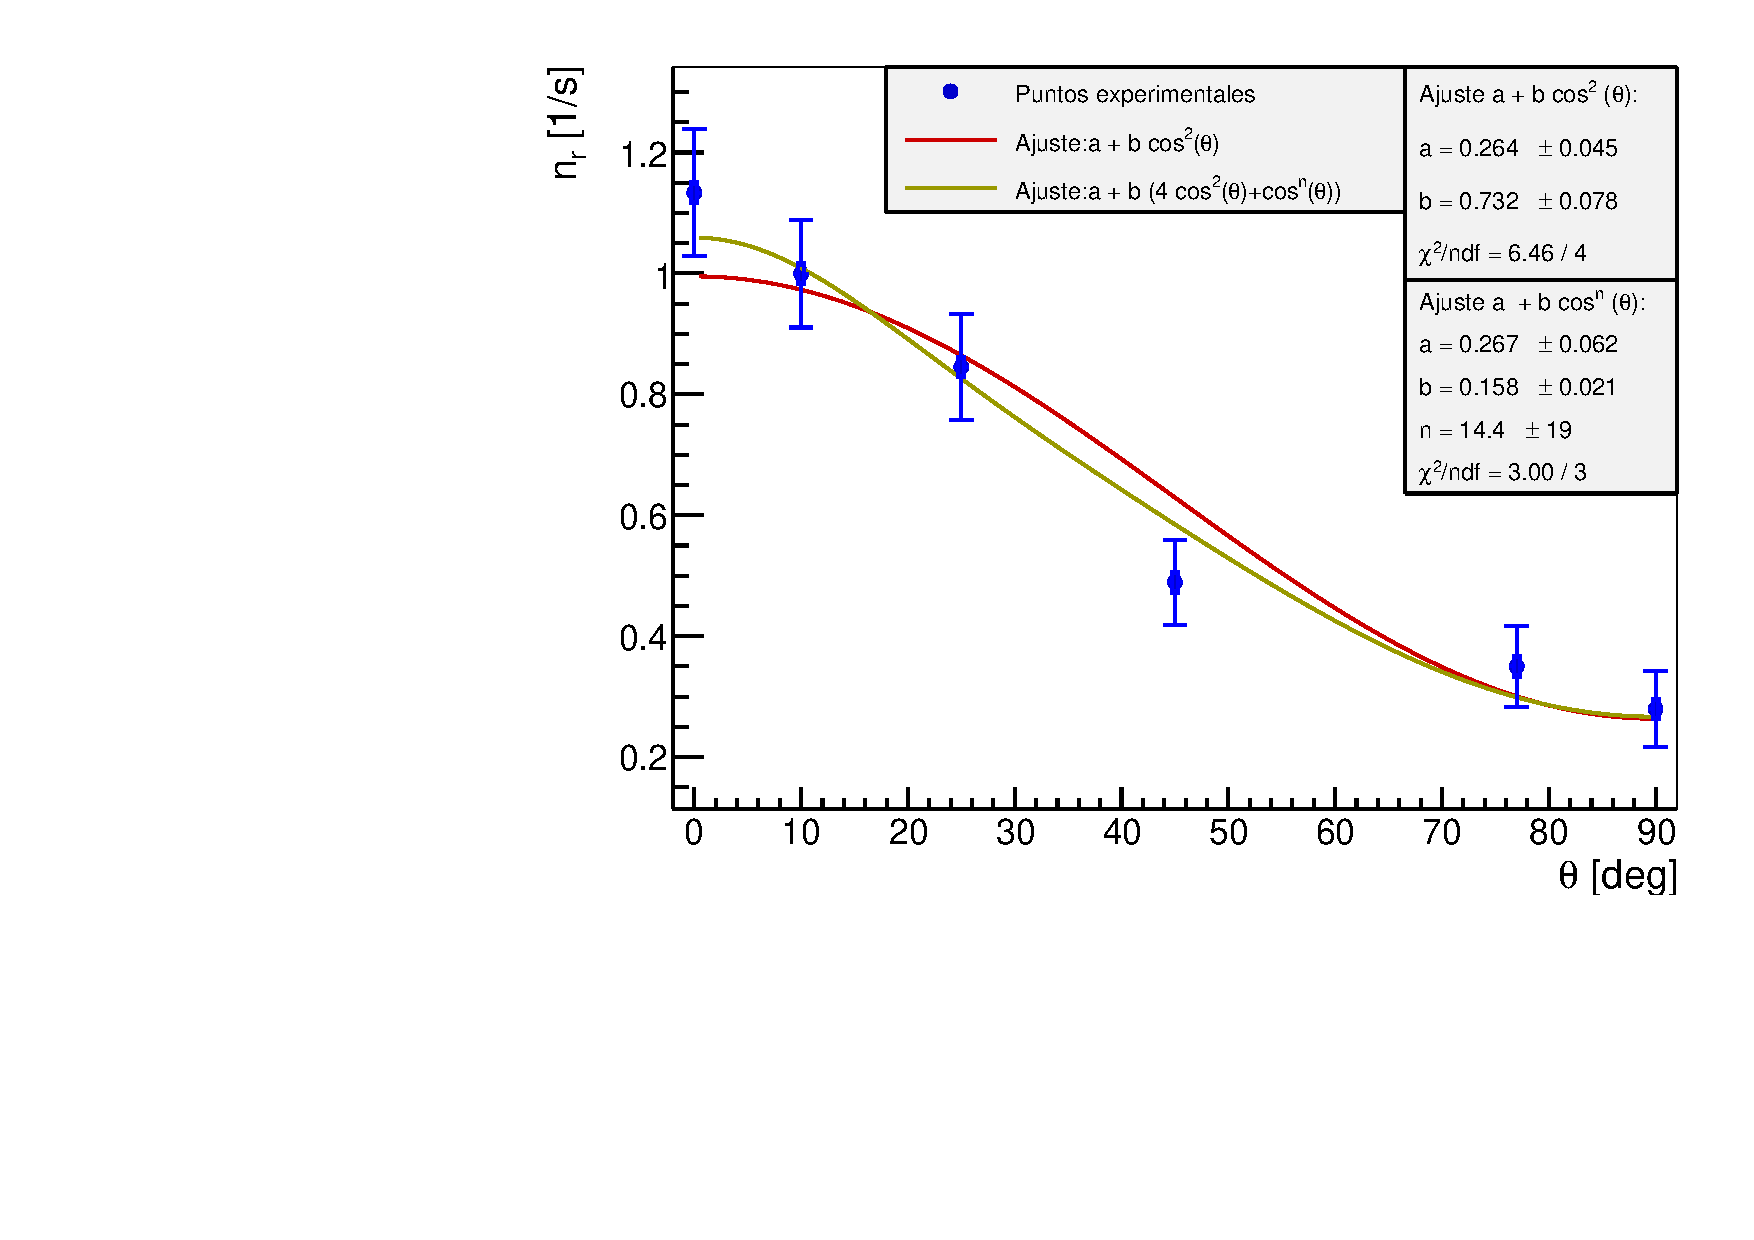
\includegraphics[width=0.99\linewidth]{../Graficas/Angulos_4.pdf}
	\end{center}
\end{minipage}


\section{Eficiencia geométrica}

\subsection{Toma de medidas y valor real de la distancia $d$}

Para tomar cada medida simpelemente separamos los detectores una distancia $d$ a través de un mueble de manera tratando  qeu es la que tomaremos como base, ya que con tan poca distanciade superponer al máximo las superficies activas, tapándo en cada medida el conjutno con una lona. Las medidas de la distancia se realizaron entre el borde de metal que proteje a un centelleador y el otro. Luego medimos la distancia entre el centelleador real y la parte de metal (con una regla), obteniendo una distancia $d_1=0.500(28)$ cm. Además el grosor del centelleador $d_2=1.7950(14)$ cm (medido con un calibrador) también será un valor de interés, ya que si la medida se realiza en la superficie externa o interna del detector superior cambia el valor real de $d$ (es decir, más cerca o más lejos del otro detector). Nostros tendremos en cuenta estos valores, de tal modo que sumaremos a la distancia $d$ realmente medida 2 veces el valor $d_1$ (ya que hay dos protectores de metal) y una vez $d_2$ (supondremos que en promedio las detecciones se hacen en medio del centelleador, que, aunque no sea verdad, es mejor que tomar un valor límite como las superficies externas):

\begin{equation}
	d_{\text{real}} = d_{\text{medida}} + 2 \cdot d_1 + d_2 
\end{equation}
tal que
\begin{equation}
	u(d_{\text{real}}) = \sqrt{u(d_{\text{medida}})^2 + (2 u(d_1))^2 + u(d_2)^2}
\end{equation}
obteniedo $u(d_{\text{real}})=2.1$ mm para cada medida. Esto que acabaos de contar hace que jamás tengamos una distancia $d=0$, lo cual es cierto, las superficies de contacto nunca estarán pegadas. El valor más pequeño que se puede alcanzar es $d_0=2.80(21)$ cm, que tomaremos como referencia para los resultados posteriores. Los obsevables están en la \cref{Tab:distancia}.

\begin{center}
\begin{table}[H]
\caption{Medidas de coincidencias a una distancia $d$ entre los detectores.}
\label{Tab:distancia}
\footnotesize
\begin{tabular}{cccccccccccccccccccccc}
\toprule
$d_{\text{real}}$ (cm) & $N_1$  & $N_2$ & $N_{12}$ & $t$ [s] & $n_1$ [s$^{-1}$] & $n_2$  [s$^{-1}$] & $n_{acc}$ [s$^{-1}$] & $n_{r}$ [s$^{-1}$] \\
\midrule
\num{2.7950000000(0.2100000000)} & \num{10319.0000000000(101.5824788042)} & \num{4468.0000000000(66.8430998683)} & \num{301.0000000000(17.3493515729)} & \num{41.1600000000(0.1300000000)} & \num{250.7045675413(2.5919038702)} & \num{108.5519922255(1.6597784794)} & \num{0.7478539177(0.0169783229)} & \num{6.5650712523(0.4224836365)} \\
\num{6.0950000000(0.2100000000)} & \num{8569.0000000000(92.5688932633)} & \num{3684.0000000000(60.6959636220)} & \num{212.0000000000(14.5602197786)} & \num{35.7400000000(0.1300000000)} & \num{239.7593732513(2.7329442325)} & \num{103.0777839955(1.7391596504)} & \num{0.6791370071(0.0156922779)} & \num{5.2525921479(0.4082654631)} \\
\num{6.0950000000(0.2100000000)} & \num{16455.0000000000(128.2770439323)} & \num{7216.0000000000(84.9470423264)} & \num{408.0000000000(20.1990098767)} & \num{69.1100000000(0.1300000000)} & \num{238.0986832586(1.9093998095)} & \num{104.4132542324(1.2447501412)} & \num{0.6831708914(0.0149963837)} & \num{5.2204609998(0.2928684246)} \\
\num{11.0950000000(0.2100000000)} & \num{22589.0000000000(150.2963738751)} & \num{9313.0000000000(96.5038859321)} & \num{411.0000000000(20.2731349327)} & \num{80.6500000000(0.1300000000)} & \num{280.0867947923(1.9174711458)} & \num{115.4742715437(1.2109668395)} & \num{0.8887806551(0.0192571525)} & \num{4.2073135793(0.2522421291)} \\
\num{11.0950000000(0.2100000000)} & \num{24440.0000000000(156.3329779669)} & \num{9925.0000000000(99.6242942259)} & \num{430.0000000000(20.7364413533)} & \num{89.9100000000(0.1300000000)} & \num{271.8273829385(1.7826391098)} & \num{110.3881659437(1.1194811437)} & \num{0.8245793415(0.0178137531)} & \num{3.9579809966(0.2314257978)} \\
\num{16.3950000000(0.2100000000)} & \num{29857.0000000000(172.7917822120)} & \num{12252.0000000000(110.6887528162)} & \num{416.0000000000(20.3960780544)} & \num{113.4800000000(0.1300000000)} & \num{263.1036305957(1.5522072527)} & \num{107.9661614381(0.9832135908)} & \num{0.7806048233(0.0167362779)} & \num{2.8852393784(0.1805591813)} \\
\num{21.5950000000(0.2100000000)} & \num{37079.0000000000(192.5590818424)} & \num{15964.0000000000(126.3487237767)} & \num{406.0000000000(20.1494416796)} & \num{141.6800000000(0.1300000000)} & \num{261.7094861660(1.3801636594)} & \num{112.6764539808(0.8977623996)} & \num{0.8103438941(0.0172485076)} & \num{2.0552687541(0.1432842454)} \\
\num{26.2950000000(0.2100000000)} & \num{48584.0000000000(220.4177851263)} & \num{20692.0000000000(143.8471410908)} & \num{419.0000000000(20.4694894905)} & \num{190.6800000000(0.1300000000)} & \num{254.7933710929(1.1689357556)} & \num{108.5168869310(0.7580094256)} & \num{0.7598050570(0.0160767553)} & \num{1.4375937263(0.1085574472)} \\
\num{30.9950000000(0.2100000000)} & \num{37162.0000000000(192.7744796388)} & \num{16595.0000000000(128.8215820428)} & \num{313.0000000000(17.6918060130)} & \num{152.2400000000(0.1300000000)} & \num{244.1014188124(1.2832952513)} & \num{109.0055176038(0.8512785517)} & \num{0.7311988734(0.0155524141)} & \num{1.3247653936(0.1172591881)} \\
\num{36.0950000000(0.2100000000)} & \num{44041.0000000000(209.8594767934)} & \num{18297.0000000000(135.2664038111)} & \num{324.0000000000(18.0000000000)} & \num{172.8000000000(0.1300000000)} & \num{254.8668981481(1.2295074061)} & \num{105.8854166667(0.7868344241)} & \num{0.7415941781(0.0157292873)} & \num{1.1334058219(0.1053569869)} \\
\num{40.9950000000(0.2100000000)} & \num{53537.0000000000(231.3806387752)} & \num{23429.0000000000(153.0653455228)} & \num{338.0000000000(18.3847763109)} & \num{218.3000000000(0.1300000000)} & \num{245.2450755841(1.0699349806)} & \num{107.3247824095(0.7040765782)} & \num{0.7232976278(0.0152710543)} & \num{0.8250303612(0.0855962423)} \\
\num{50.9950000000(0.2100000000)} & \num{59969.0000000000(244.8856876177)} & \num{26718.0000000000(163.4564162093)} & \num{325.0000000000(18.0277563773)} & \num{243.6300000000(0.1300000000)} & \num{246.1478471453(1.0136990854)} & \num{109.6662972540(0.6734678292)} & \num{0.7417984993(0.0156291432)} & \num{0.5921915676(0.0756323487)} \\
\num{57.2950000000(0.2100000000)} & \num{44514.0000000000(210.9834116702)} & \num{19942.0000000000(141.2161463856)} & \num{210.0000000000(14.4913767462)} & \num{180.4000000000(0.1300000000)} & \num{246.7516629712(1.1829712455)} & \num{110.5432372506(0.7868373835)} & \num{0.7495644750(0.0158769298)} & \num{0.4145153476(0.0818874302)} \\
\bottomrule
\end{tabular}
\end{table}
\end{center}


\subsection{Eficiencia geométrica}

En este apartado trataremos de estudiar la eficiencia geométrica de neustro experimento. Así pues compararemos los datos tomados en la práctica y los contrastaremos con un estudio Monte Carlo. Para esto último nos basaremos en el artículo N8 \cite{N8}. Definimos como eficiencia $\epsilon_T$ la tasa de eventos detectados y la tasa de eventos realmente ocurrentes, tal que:

\begin{equation}
	\epsilon_T = \frac{J_{\text{detectadas}}}{J_{\text{reales}}}
\end{equation}
Podemos separar la eficiencia total en eficiencia intrínseca $\epsilon_i$ y la eficiencia geométrica $\epsilon_g$, tal que:

\begin{equation}
	\epsilon_t = \epsilon_g \times \epsilon_i
\end{equation}
Definimos eficiencia geométrica $\epsilon_g$ como el cociente entre el número de sucesos que llegan al detector y el número de sucesos que es emitidos por la fuente y relacionarlo con la distancia que separa los detectores $d$ \cite{Raul} tal que 

\begin{equation}
	\epsilon_g (d) = \frac{J(d)}{J(0)} \tquad 
	u(\epsilon_g(d)) = \sqrt{\parentesis{\frac{u(J(d))}{J(0)}}^2+\parentesis{\frac{J(d)u(J(0))}{J(0)^2}}^2}
\end{equation}
siendo $J(d)$ el flujo de rayos cósmicos incidentes cuando los detectores estan separados una distancia $d$. Lógicamente el flujo se relaciona con nuestros datos tal y como hemos descrito previamente: 

\begin{equation}
	J(d) = \frac{n_r(d)}{A}
\end{equation}
siendo $A=300$ m$^2$. Así pues, a través de un Monte Carlo vamos a tratar de calcular $\epsilon_g(d)$ para las mismas distancias que las que tenemos. 

Se trata de determinar cual es la mejor aproximación a los resultados experimentales. Para esto calcularemos (véase N6 \cite{N6})

\begin{equation}
	\chi^2_{\text{MC}} = \sum_i \frac{\parentesis{\epsilon_T(d_i)- P_{\
	\text{MC}} \epsilon_{MC}(d_i)}}{\ccorchetes{u(E_t(d_i))}^2}
\end{equation}
tratando de obtener el valor $P$ que minimize $\chi^2$. Así, el valor $P$ corresponderá al multiplicador a aplicar a $\epsilon_g$ para que las distancias entre $\epsilon_T$ y $\epsilon_g$ sean mínimas. De esta forma, minimizando el $\chi^2$ en cada una delas aproxiaciones encontraremos cual es la mejor y encontraremos el mejor parámetro $P$ para cada uno. ¿El significado de $P$? Queda claro que es la eficiencia intrínseca tal que:

\begin{equation}
	P \equiv \epsilon_i
\end{equation}
en este apartado nuestro principal objetivo será obtner $\chi^2$ para nuestro montecarlo, el parámetro $P$ para cada aproximación y cuál será la mejor aproximación (y por qué) en función de $\chi^2$ \cite{N6}. Como nostros vamos a hacerlo en un principio para la tasa: 

\begin{equation}
	\chi^2_{\text{MC}} = \sum_i \frac{\parentesis{n_r(d_i)- \alpha \epsilon_{\text{MC}} (d_i)}}{\ccorchetes{u(n_r(d_i))}^2}
\end{equation}
Para nosotros:

\begin{equation}
	\epsilon_g(d=2.8 \unit{cm}) = 1
\end{equation}
de lo que se deduce que
\begin{equation}
	\epsilon_i = \alpha / n_r
\end{equation}
usando el valor obtenido en el apartado \ref{Subsec:6.5} $n_r=7.51(18)$ s$^{-1}$. El valor: 

\begin{equation}
	\epsilon_g(d_i) = \frac{n_r(d_i)}{n_r(d_0)}  \qquad 
	\epsilon_{\text{MC}}(d_i) = \frac{n_\text{MC}(d_i)}{n_r(d_0)}
\end{equation}

\subsection{Resulados de Monte Carlo y contraste con los datos}

Los resultados de montecarlo los presentamos en la tabla \cref{Tab:montecarlo} (con $N=10^7$ pruebas por posición) donde indicamos con superíndice 1 al de $n=2$ y con superíndice $2$ al obtenido con $n=4.73$. Como podemos 

\begin{equation}
n = 2: \  \alpha_{MC} =  7.48425 \quad \chi^2 =8.63226 \qquad 
n = 4.63 : \  \alpha_{MC} = 6.19439 \quad \chi^2 = 24.837
\end{equation}
para 11 grados de libertad. Así podemos ver que el resultado para $n=2$ es bastante bueno y es compatible con los datos, mientras que para $n=4.63$ no lo es porque $\chi^2_{0.999,11}= 24.725$ lo cual vemos que sobrepasa completamente, siendo no compatibles con los datos.\textcolor{blue}{Esto nos da información acerca de que quizás la falta de sensibilidad en el método anterior podría ser corregido aquí, ya que si parece que somos sensibles a uno u otro exponente con este método.} Obtenemos a partir del dato concluyente de $\epsilon_i$ usando qeu $n_r=7.51(18)$ s$^{-1}$. así pues: 

\begin{equation}
	\epsilon_i = 0.996(23)
\end{equation}
lo cual es un resultado físico $\epsilon_i<1$ y que cuadra con el guion \cite{P2} que dice ``la eficiencia intrínseca de los plásticos orgánicos gruesos para partículas cargadas energéticas a las energñias de los rayos cósmicos es cercana del 100\%''.

\begin{figure}[h!]
	\centering
	\captionof{figure}{Montecarlo para $n=2$ y $n=4.63$}
	\label{Fig:montecarlo}
	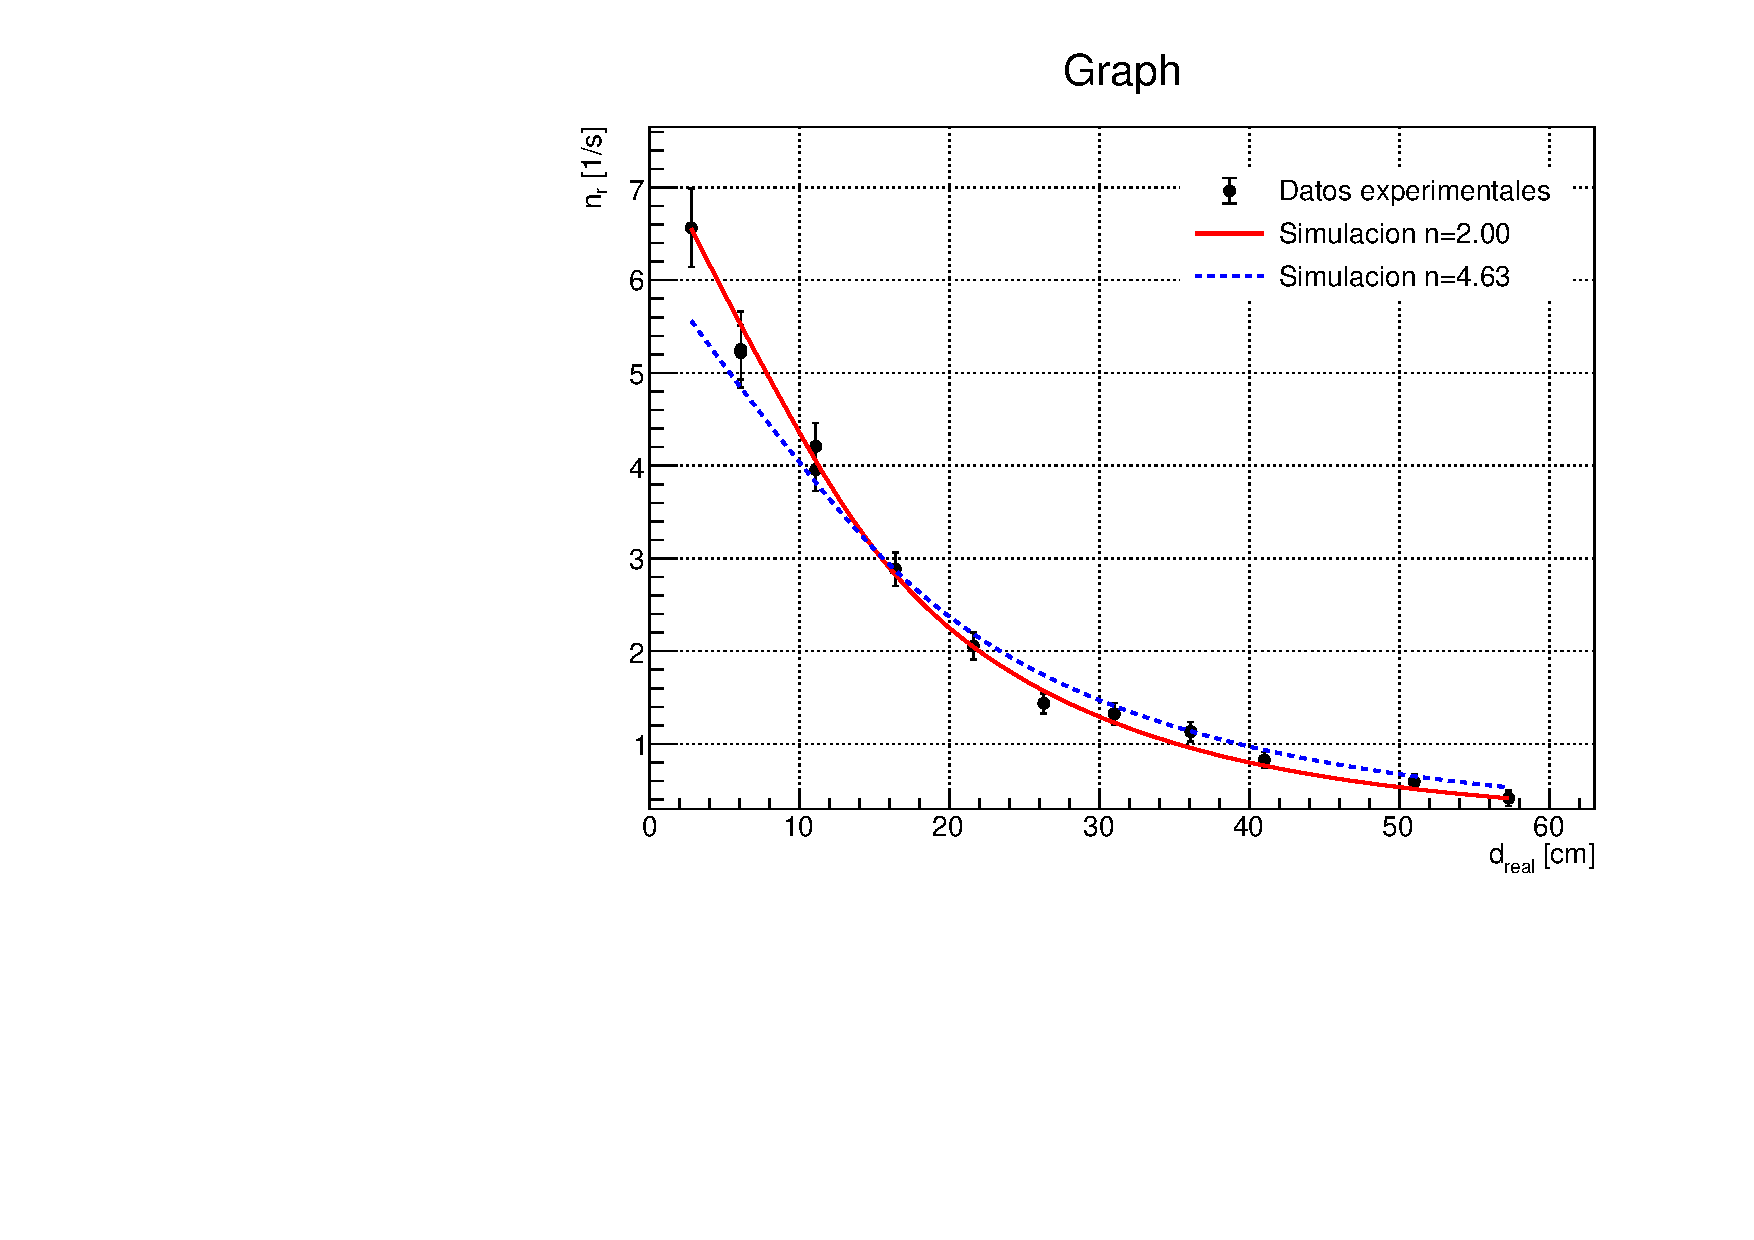
\includegraphics[width=0.7\linewidth]{../Graficas/Montecarlo.pdf}
\end{figure}


\begin{center}
\begin{table}[H]
\caption{Medidas de la eficiencia.}
\label{Tab:montecarlo}
\centering
\begin{tabular}{cccccccccccccccccccccc}
\toprule
$d_{\text{real}}$ (cm) & $\epsilon_{g}$ & $\epsilon_{\text{MC}}^1$ & $\epsilon_{\text{MC}}^2$ \\
\midrule
\num{2.7950000000(0.2100000000)} & \num{1.0000000000(0.0643532447)} & \num{0.9989899192(0.0001186918)} & \num{0.8471347509(0.0000903692)} \\
\num{6.0950000000(0.2100000000)} & \num{0.8000815141(0.0621875144)} & \num{0.8402010866(0.0001587142)} & \num{0.7376386050(0.0001232390)} \\
\num{6.0950000000(0.2100000000)} & \num{0.7951872568(0.0446100908)} & \num{0.8403366526(0.0001586898)} & \num{0.7377680780(0.0001232113)} \\
\num{11.0950000000(0.2100000000)} & \num{0.6408633536(0.0384218418)} & \num{0.6170793651(0.0001796355)} & \num{0.5817453997(0.0001450761)} \\
\num{11.0950000000(0.2100000000)} & \num{0.6028846976(0.0352510718)} & \num{0.6171890364(0.0001796325)} & \num{0.5819723584(0.0001450589)} \\
\num{16.3950000000(0.2100000000)} & \num{0.4394833304(0.0275030041)} & \num{0.4304858076(0.0001747689)} & \num{0.4378627268(0.0001488005)} \\
\num{21.5950000000(0.2100000000)} & \num{0.3130611497(0.0218252384)} & \num{0.3123027795(0.0001607781)} & \num{0.3335074237(0.0001426356)} \\
\num{26.2950000000(0.2100000000)} & \num{0.2189761042(0.0165356084)} & \num{0.2394764565(0.0001468525)} & \num{0.2652644477(0.0001341349)} \\
\num{30.9950000000(0.2100000000)} & \num{0.2017899491(0.0178610686)} & \num{0.1872850960(0.0001335781)} & \num{0.2148643854(0.0001251264)} \\
\num{36.0950000000(0.2100000000)} & \num{0.1726418158(0.0160481102)} & \num{0.1456291887(0.0001203373)} & \num{0.1731466356(0.0001154947)} \\
\num{40.9950000000(0.2100000000)} & \num{0.1256696736(0.0130381285)} & \num{0.1165207460(0.0001092052)} & \num{0.1423760633(0.0001068017)} \\
\num{50.9950000000(0.2100000000)} & \num{0.0902033725(0.0115204155)} & \num{0.0786095048(0.0000913434)} & \num{0.0993283964(0.0000915719)} \\
\num{57.2950000000(0.2100000000)} & \num{0.0631395048(0.0124731975)} & \num{0.0628678630(0.0000822907)} & \num{0.0810135914(0.0000835919)} \\
\bottomrule
\end{tabular}
\end{table}
\end{center}


\section{Conclusiones}

Durante esta memoria hemos tratado de caracterizar detalladamente tanto los detectores como la radiación cósmica. Como en la mayor parte de los apartados ya hemos incluido algunas conclusiones, aquí nos limitaremos a resumirlas y a comentar, finalmente, nuestras sensaciones y posibles mejoras de cara al futuro. 

En la primera parte caracterizamos nuestro detector, obteniendo una ventaa de coincidencias $\tau_13.74(57)$ s$^{-1}$ que era un valor concluyente, ya que está en el orden de lo que nos imaginábamos. Esta ventana de coincidencias es fundamental ya que la hemos usado en todos los apartados posteriores para calcular $n_r$ a partir de $n_{12}$. Consecuentemente me hubiera gustado tomar más medidas de la misma, ya que tomamos 3 medidas cada una con un $5/10$ \% de incertidumbre relativa. 

Luego caracterizamos el comportamiento de $n_r$ frente a $U_{1,2}$ y $V_{1,2}$ obteniendo un resultado extraño, ya que el alto voltaje no parecía mostrar ningún \textit{plateu} claro, lo cual nos dejo ciertas dudas para elegir adecuadaente $V_1$ y $V_2$ para los siguientes apartados. Nosotros elegimos un alto voltaje alto, por razones explicadas anteriormente, aunque con cierta desconfianza. De hecho este creo que es el primer aspecto que mejoraría de esta práctica, haber tomado más datos y con mayor tiempo para obtener así un valor de $V$ y $U$ con ciertas garantías, minimizando las accidentales.

Posteriormente tratamos de caracetrizar la distribucción que seguía nuestros datos. Las conclusiones extraidas en este apartado eran claras: los datos siguen una distribución de poisson para coincidencias medidas en un intervalo temporal mayor a 1s. Un análisis que nos hubiera gustado hacer sería incluir el ajueste binomial de alguna forma, ya que en \cite{Knoll:1300754} afrimaba que este es el \textit{modelo más general y con mayores campos de aplicación}. 

La caracterización de la compontente dura y blanda fue un éxito parcial, ya que no tomamos los datos de los bloques de plomo, lo cual no nos permitió caracterizar adecuadamente $\lambda_m^\mu$, e incluso con los datos de Celtia Jabares tampoco obtuvimos el resultado esperado. Sin embargo, los resultados obtenidos con nuestros propios datos frenando la radiación electrónica solo con las planchas de hierro fue sorprendentemente bien, obteniendo un flujo electrónica $J_e=50$ m$^{-2}$s$^{-1}$, y un valor de flujo muónico compatible con los datos  de Jeng-Wei Lin \cite{LIN201024}. De hecho que los resultados sean compatibles con un frenado electrónico únicamente con 20 planchas de hierro es un éxito, y lo considero uno de los grandes resutlados de esta práctica.

Luego estudiamos la distribucción angular de los rayos cósmicos enfrentando varios modelos, obteniendo como resultado que $j_1(\theta)\propto cos^2(\theta)$ es efectivamente compatible con los datos pero que el mejor ajuste a la distribución angular del flujo en la superficie terrestre para nuestros datos es $j_2(\theta)\propto cos^4.63(\theta)$. También tratamos de diferenciar componetne electrónica y muónica con nuestros datos, para ver si la componente blanda seguía la misma relación que la muónica, aunque sin ningún resultado concluyente.

Finalmente estudiamos la eficiencia geométrica, donde podríamos en el punto de mira los resultados obtenidos en el apartado anterior. La eficiencia geométrica puso en entredicho directamente que $j_2$ sera la mejor forma de describir la tasa, ya que como podemos ver en \cref{Fig:montecarlo} ni siquiera es compatible con los resultados, mientras que $j_1$ es compatible tanto con la distribución angular como con la eficiencia geométrica. Nuestro estudio de montecarlo describe perfectamente la distribución geométtrica obtenida, con un $\chi^2$/ndf$<$1. Como resultado concluimos que nuestros datos son compatibles con una distribución $j(\theta)\propto \cos^2(\theta)$. 

Lógicamente faltarían tomar más medidas para obtenr un buen estudio en todos los puntos. Un factor que me parece interesante a mejorar de cada a futuro es la disposición, debiendo estar todo el aparataje de medida en la parte más adentro del laboratorio, ya que al medir rayos cósmicos debería estar pegado a la ventana al lado de rayos cósmicos digital. Otro factor podría ser que el aparato experimental estar mas aislado del resto del laboratorio, ya que hay fuentes de electrones que pueden afectar a nuestras medidas. 

para final me gustaría agradecer la ayuda de Celtia Jabares por pasarme sus datos de la atenuación y a mi padre por ayudarme a realizar la red neuronal. También fue de vital importancia la memoria de Raul Lois \cite{Raul}.

\newpage

\appendix

\section{Codigo y Método Monte Carlo}

En este apartado comentaremos un poco en qué nos hemos basado para desarrollar el código, qué hemos tenido en cuenta y, finalmente, escribiremos el código. 

\subsection{Método Monte Carlo}

Para simular direcciones aleatorias de incidencia de rayos cósmicos, se tiene en cuenta que la densidad de probabilidad asociada a una dirección dada por los ángulos $\theta$ y $\phi$ se puede obtener como el producto de dos distribuciones angulares independientes. En particular, se asume que la distribución en $\theta$ (ángulo polar) está modulada por un factor $\cos^{n+1}\theta$, el cual proviene de considerar el ángulo de incidencia respecto a un detector plano \cite{N8}.

La función de densidad de probabilidad toma la forma:

\begin{equation}
f(\theta, \phi) \D  \theta \D \phi = A (\cos\theta)^{n+1} \frac{1}{2\pi} \sin\theta \D \theta \D  \phi
\end{equation}

donde $A$ es una constante de normalización, que se se determina imponiendo la condición de que la integral total sobre el hemisferio sea 1. De ahí se obtiene:

\begin{equation}
A = n + 2
\end{equation}
Así, la función de distribución acumulada $F(\theta, \phi)$ se calcula integrando la densidad de probabilidad, dando como resultado:

\begin{equation}
F(\theta, \phi) = \iint f(\theta,\phi) \D  \theta \D \phi = \frac{\phi}{2\pi} \left( 1 - \cos^{n+2}\theta \right)
\end{equation}
Dado que las variables $\theta$ y $\phi$ son estadísticamente independientes, se pueden generar de forma separada utilizando variables aleatorias uniformes $u_1, u_2 \in [0,1]$. Aplicando la inversa de la función acumulada se obtienen:

\begin{equation}
\theta = \arccos\left( (1 - u_1)^{\frac{1}{n+2}} \right), \qquad \phi = 2\pi u_2
\end{equation}
Para determinar el punto en el que el rayo cósmico incide en el primer detector, se generan coordenadas aleatorias $(x_1, y_1)$ dentro del área activa del mismo, usualmente delimitada por $x_1 \in [0,30]\,\mathrm{cm}$ y $y_1 \in [0,10]\,\mathrm{cm}$.

Luego, empleando consideraciones geométricas y suponiendo una trayectoria rectilínea, la posición en el segundo detector separado una distancia $d$ se calcula como:

\begin{equation}
x_2 = x_1 - d \tan\theta \cos\phi, \qquad y_2 = y_1 - d \tan\theta \sin\phi
\end{equation}
Se registra una coincidencia si las coordenadas $(x_2, y_2)$ también se encuentran dentro del área activa del segundo detector, es decir, si $x_2 \in [0,30]\,\mathrm{cm}$ y $y_2 \in [0,10]\,\mathrm{cm}$. Nosotros no consideraremos aquí el grosor del detector, ya que habría que aumentar la distancia $d$ usada en una variable aleatoria nueva tal qeu $d=d+u_3$ siendo $u_3\in [-0.7975,0.7975]$ el cual es bastante pequeño en comparación de las distancias tomadas. Se puede dejar para un revisión posterior, si hiciera falta. 

\subsection{Codigo}

El código usado fue el presentado justo abajo. Es importante mencionar dos puntos: sin la ayuda de las inteligencias artificiales (chatGPT) este código no habría sido posible, ya que nos ayudo a depurar los numerosos fallos en cada momento y a comentar cada paso que hacíamos (aunque el código dipuesto abajo está sin comentar). También fue de gran ayuda e inspiración el código realizado por Raúl Lois Coins \cite{Raul}, del que tomamos alguna idea. \\[1em] 

\begin{lstlisting}[language=C++, caption={Simulación Monte Carlo de eficiencia de detección en C++ROOT \cite{Root}. Formato \href{https://ctan.org/pkg/listings}{lstlisting} basado en \href{https://gist.github.com/mpdehnel/cc43e89a09c18ef6a602}{
mpdehnel}} Martin Dehnel-Wil.]
#include <iostream>
#include <fstream>
#include <sstream>
#include <vector>
#include <cmath>
#include <string>
#ifndef M_PI
#define M_PI 3.14159265358979323846
#endif
#include "TRandom3.h"
#include "TCanvas.h"
#include "TGraphErrors.h"
#include "TGraph.h"
#include "TLegend.h"
#include "TAxis.h"
#include "TROOT.h"
#include "TApplication.h"
#include "TString.h"

const int Nparticles = 10000000;
const double detectorRadius = 10.0;

void SetEstiloPublicacion() {
    gStyle->SetOptStat(0);
    gStyle->SetOptTitle(0);
    gStyle->SetTitleFont(42, "XYZ");
    gStyle->SetLabelFont(42, "XYZ");
    gStyle->SetTitleSize(0.05, "XYZ");
    gStyle->SetLabelSize(0.045, "XYZ");
    gStyle->SetFrameLineWidth(1.3);
    gStyle->SetLineWidth(2.3);
    gStyle->SetHistLineWidth(1.3);
    gStyle->SetTickLength(0.03, "X");
    gStyle->SetTickLength(0.03, "Y");
}

bool LeerDatosCSV(const char* filename,
                  std::vector<double> &dist, std::vector<double> &errDist,
                  std::vector<double> &rate, std::vector<double> &errRate)
{
    std::ifstream infile(filename);
    if (!infile.is_open()) {
        std::cerr << "No se pudo abrir el archivo: " << filename << std::endl;
        return 1;
    }

    std::string linea;
    std::getline(infile, linea); // saltar cabecera

    std::vector<double> x, sx, y, sy;

    while (std::getline(infile, linea)) {
        std::stringstream ss(linea);
        std::string campo;
        std::vector<double> fila;

        while (std::getline(ss, campo, ',')) {
            fila.push_back(std::stod(campo));
        }

        if (fila.size() == 4) {
            x.push_back(fila[0]);
            sx.push_back(fila[1]);
            y.push_back(fila[2]);
            sy.push_back(fila[3]);
        }
    }

    dist = x; errDist = sx;
    rate = y; errRate = sy;

    return true;
}

double SimularEficiencia(double n, double d, TRandom3 &randGen)
{
    long long countCoincident = 0;
    for (int i = 0; i < Nparticles; ++i)
    {
        double x1 = randGen.Uniform()*30;
        double y1 = randGen.Uniform()*10;
        double r = detectorRadius * std::sqrt(std::pow(x1,2)+std::pow(y1,2));
        double u2 = randGen.Uniform();
        double cosTheta = std::pow(u2, 1.0 / (n + 2.0));
        double sinTheta = std::sqrt(1 - cosTheta * cosTheta);
        double phi_dir = randGen.Uniform(0, 2 * M_PI);
        double x2 = x1 + d * (sinTheta * std::cos(phi_dir));
        double y2 = y1 + d * (sinTheta * std::sin(phi_dir));
        if (x2 > 0 && x2 < 30 && y2 > 0 && y2 < 10) {
            countCoincident++;
        }
    }
    return (double)countCoincident / (double)Nparticles;
}

int Montecarlo()
{
    const char* nombreArchivo = "Distancias.csv";

    std::vector<double> dist, errDist, rate, errRate;
    if (!LeerDatosCSV(nombreArchivo, dist, errDist, rate, errRate)) return 1;
    int Npoints = dist.size();
    if (Npoints == 0) return 1;

    TRandom3 randGen;
    randGen.SetSeed(0);
    double n1 = 2.0;
    double n2 = 4.63;
    std::vector<double> eff_n1, eff_n2;
    eff_n1.reserve(Npoints);
    eff_n2.reserve(Npoints);

    for (int i = 0; i < Npoints; ++i) {
        eff_n1.push_back(SimularEficiencia(n1, dist[i], randGen));
        eff_n2.push_back(SimularEficiencia(n2, dist[i], randGen));
    }

    double chi2_n1 = 0.0, chi2_n2 = 0.0;
    double scale_n1 = 1.0, scale_n2 = 1.0;

    {
        double num = 0.0, den = 0.0;
        for (int i = 0; i < Npoints; ++i) {
            double sigma = (errRate[i] == 0.0 ? 1.0 : errRate[i]);
            num += rate[i] * eff_n1[i] / (sigma * sigma);
            den += eff_n1[i] * eff_n1[i] / (sigma * sigma);
        }
        if (den != 0.0) scale_n1 = num / den;

        for (int i = 0; i < Npoints; ++i) {
            double sigma = (errRate[i] == 0.0 ? 1.0 : errRate[i]);
            double diff = eff_n1[i] * scale_n1 - rate[i];
            chi2_n1 += (diff * diff) / (sigma * sigma);
        }
    }

    {
        double num = 0.0, den = 0.0;
        for (int i = 0; i < Npoints; ++i) {
            double sigma = (errRate[i] == 0.0 ? 1.0 : errRate[i]);
            num += rate[i] * eff_n2[i] / (sigma * sigma);
            den += eff_n2[i] * eff_n2[i] / (sigma * sigma);
        }
        if (den != 0.0) scale_n2 = num / den;

        for (int i = 0; i < Npoints; ++i) {
            double sigma = (errRate[i] == 0.0 ? 1.0 : errRate[i]);
            double diff = eff_n2[i] * scale_n2 - rate[i];
            chi2_n2 += (diff * diff) / (sigma * sigma);
        }
    }

    std::cout << "Resultado del ajuste:\n";
    std::cout << "  n = " << n1 << " -> escala = " << scale_n1 << ", chi-cuadrado = " << chi2_n1 << std::endl;
    std::cout << "  n = " << n2 << " -> escala = " << scale_n2 << ", chi-cuadrado = " << chi2_n2 << std::endl;

    TGraphErrors *grData = new TGraphErrors(Npoints, dist.data(), rate.data(), errDist.data(), errRate.data());
    grData->GetXaxis()->SetTitle("d_{real} [cm]");
    grData->GetYaxis()->SetTitle("n_{r} [1/s]");
    grData->SetMarkerStyle(20);
    grData->SetMarkerColor(kBlack);
    grData->SetLineColor(kBlack);
    grData->SetLineWidth(1);

    int NcurvePoints = 100;
    double d_min = *std::min_element(dist.begin(), dist.end());
    double d_max = *std::max_element(dist.begin(), dist.end());
    double step = (d_max - d_min) / (NcurvePoints - 1);
    std::vector<double> curve_d, curve_sim1, curve_sim2;

    for (int j = 0; j < NcurvePoints; ++j)
    {
        double d_val = d_min + j * step;
        double eff1 = SimularEficiencia(n1, d_val, randGen);
        double eff2 = SimularEficiencia(n2, d_val, randGen);
        curve_d.push_back(d_val);
        curve_sim1.push_back(eff1 * scale_n1);
        curve_sim2.push_back(eff2 * scale_n2);
    }

    TGraph *grSim1 = new TGraph(NcurvePoints, curve_d.data(), curve_sim1.data());
    TGraph *grSim2 = new TGraph(NcurvePoints, curve_d.data(), curve_sim2.data());
    grSim1->SetLineColor(kRed); grSim1->SetLineWidth(2); grSim1->SetLineStyle(1);
    grSim2->SetLineColor(kBlue); grSim2->SetLineWidth(2); grSim2->SetLineStyle(2);

    TCanvas *c1 = new TCanvas("c1", "Simulacion vs Datos", 800, 600);
    c1->SetGrid();
    grData->Draw("AP");
    grSim1->Draw("L SAME");
    grSim2->Draw("L SAME");

    TLegend *legend = new TLegend(0.55, 0.7, 0.88, 0.85);
    legend->SetBorderSize(0); legend->SetFillColor(0);
    legend->AddEntry(grData, "Datos experimentales", "PE");
    legend->AddEntry(grSim1, TString::Format("Simulacion n=%.2f", n1), "L");
    legend->AddEntry(grSim2, TString::Format("Simulacion n=%.2f", n2), "L");
    legend->Draw();

    c1->SetRightMargin(0.03);
    c1->SetTopMargin(0.03);
    c1->Update();
    c1->SaveAs("../Graficas/Montecarlo.pdf");

    std::ofstream outfile("../Datos Crudos/Eficiencias.csv");
    if (!outfile.is_open()) {
        std::cerr << "No se pudo crear el archivo de salida Montecarlo_resultados.csv" << std::endl;
    } else {
        outfile << "distancia,sim_n1,err_sim_n1,sim_n2,err_sim_n2\n";
        for (int i = 0; i < Npoints; ++i) {
            double e1 = eff_n1[i], e2 = eff_n2[i];
            double sim_n1 = e1 * scale_n1;
            double sim_n2 = e2 * scale_n2;
            double err_sim_n1 = scale_n1 * std::sqrt(e1 * (1.0 - e1) / Nparticles);
            double err_sim_n2 = scale_n2 * std::sqrt(e2 * (1.0 - e2) / Nparticles);
            outfile << dist[i] << "," << sim_n1 << "," << err_sim_n1 << ","
                    << sim_n2 << "," << err_sim_n2 << "\n";
        }
        outfile.close();
        std::cout << ">> Resultados guardados en Montecarlo_resultados.csv" << std::endl;
    }

    return 0;
}
\end{lstlisting}


\newpage

\section{Tablas} \label{Sec:tablas}

\subsection{Distribuciones}
\begin{center}
\begin{table}[H]
\caption{Valores del histograma 1ms}
\label{Tab:histo_1s}
\begin{tabular}{ccccc}
\toprule
Frecuencia & Cuentas \\
\midrule
\num{    0} & \num{28487} \\
\num{    1} & \num{13393} \\
\num{    2} & \num{ 3615} \\
\num{    3} & \num{  643} \\
\num{    4} & \num{  187} \\
\num{    5} & \num{  416} \\
\num{    6} & \num{  488} \\
\num{    7} & \num{  258} \\
\num{    8} & \num{   94} \\
\num{    9} & \num{   58} \\
\num{   10} & \num{   53} \\
\num{   11} & \num{   12} \\
\num{   12} & \num{    7} \\
\num{   13} & \num{    1} \\
\num{   14} & \num{    0} \\
\num{   15} & \num{    1} \\
\num{   16} & \num{    1} \\
\bottomrule
\end{tabular}
\end{table}
\end{center}

\begin{center}
\begin{table}[H]
\caption{Valores del histograma 2ms}
\label{Tab:histo_2s}
\begin{tabular}{ccccc}
\toprule
Frecuencia & Cuentas \\
\midrule
\num{    0} & \num{ 8366} \\
\num{    1} & \num{ 8444} \\
\num{    2} & \num{ 4287} \\
\num{    3} & \num{ 1487} \\
\num{    4} & \num{  411} \\
\num{    5} & \num{  232} \\
\num{    6} & \num{  213} \\
\num{    7} & \num{  169} \\
\num{    8} & \num{   97} \\
\num{    9} & \num{   47} \\
\num{   10} & \num{   32} \\
\num{   11} & \num{   16} \\
\num{   12} & \num{    8} \\
\num{   13} & \num{    3} \\
\num{   14} & \num{    0} \\
\num{   15} & \num{    1} \\
\num{   16} & \num{    1} \\
\num{   17} & \num{    0} \\
\num{   18} & \num{    0} \\
\num{   19} & \num{    2} \\
\num{   20} & \num{   17} \\
\num{   21} & \num{   10} \\
\num{   22} & \num{    1} \\
\num{   23} & \num{    1} \\
\num{   24} & \num{    0} \\
\num{   25} & \num{    0} \\
\num{   26} & \num{    0} \\
\num{   27} & \num{    0} \\
\num{   28} & \num{    0} \\
\num{   29} & \num{    1} \\
\num{   30} & \num{    1} \\
\num{   31} & \num{    4} \\
\num{   32} & \num{    2} \\
\num{   33} & \num{    1} \\
\num{   34} & \num{    2} \\
\bottomrule
\end{tabular}
\end{table}
\end{center}

\begin{center}
\begin{table}[H]
\caption{Valores del histograma 5ms}
\label{Tab:histo_5s}
\begin{tabular}{ccccc}
\toprule
Frecuencia & Cuentas \\
\midrule
\num{    0} & \num{  767} \\
\num{    1} & \num{ 1782} \\
\num{    2} & \num{ 2320} \\
\num{    3} & \num{ 1991} \\
\num{    4} & \num{ 1347} \\
\num{    5} & \num{  673} \\
\num{    6} & \num{  347} \\
\num{    7} & \num{  174} \\
\num{    8} & \num{   81} \\
\num{    9} & \num{   66} \\
\num{   10} & \num{   35} \\
\num{   11} & \num{   15} \\
\num{   12} & \num{    9} \\
\num{   13} & \num{    6} \\
\num{   14} & \num{    3} \\
\num{   15} & \num{    1} \\
\num{   16} & \num{    1} \\
\num{   17} & \num{    1} \\
\num{   18} & \num{    0} \\
\num{   19} & \num{    0} \\
\num{   20} & \num{    0} \\
\num{   21} & \num{    2} \\
\num{   22} & \num{    1} \\
\num{   23} & \num{    1} \\
\num{   24} & \num{    0} \\
\num{   25} & \num{    0} \\
\num{   26} & \num{    0} \\
\num{   27} & \num{    0} \\
\num{   28} & \num{    0} \\
\num{   29} & \num{    0} \\
\num{   30} & \num{    0} \\
\num{   31} & \num{    0} \\
\num{   32} & \num{    2} \\
\num{   33} & \num{    1} \\
\num{   34} & \num{    1} \\
\num{   35} & \num{    1} \\
\num{   36} & \num{    0} \\
\num{   37} & \num{    0} \\
\num{   38} & \num{    0} \\
\num{   39} & \num{    0} \\
\num{   40} & \num{    0} \\
\num{   41} & \num{    3} \\
\num{   42} & \num{    1} \\
\num{   43} & \num{    2} \\
\num{   44} & \num{    1} \\
\num{   45} & \num{    0} \\
\num{   46} & \num{    0} \\
\num{   47} & \num{    1} \\
\num{   48} & \num{    0} \\
\num{   49} & \num{    0} \\
\num{   50} & \num{    3} \\
\num{   51} & \num{    2} \\
\num{   52} & \num{    3} \\
\num{   53} & \num{    1} \\
\num{   54} & \num{    2} \\
\num{   55} & \num{    0} \\
\num{   56} & \num{    0} \\
\num{   57} & \num{    0} \\
\num{   58} & \num{    1} \\
\num{   59} & \num{    0} \\
\num{   60} & \num{    2} \\
\num{   61} & \num{    1} \\
\num{   62} & \num{    2} \\
\num{   63} & \num{    3} \\
\num{   64} & \num{    1} \\
\num{   65} & \num{    0} \\
\num{   66} & \num{    0} \\
\num{   67} & \num{    0} \\
\num{   68} & \num{    0} \\
\num{   69} & \num{    0} \\
\num{   70} & \num{    1} \\
\num{   71} & \num{    1} \\
\num{   72} & \num{    4} \\
\num{   73} & \num{    1} \\
\num{   74} & \num{    1} \\
\num{   75} & \num{    0} \\
\num{   76} & \num{    0} \\
\num{   77} & \num{    0} \\
\num{   78} & \num{    0} \\
\num{   79} & \num{    0} \\
\num{   80} & \num{    0} \\
\num{   81} & \num{    0} \\
\num{   82} & \num{    0} \\
\num{   83} & \num{    1} \\
\bottomrule
\end{tabular}
\end{table}
\end{center}

\begin{center}
\begin{table}[H]
\caption{Tabla para 7 s con $\mu=3.79$, $N=6849$, $\chi^2_{\text{Poisson}}=111.56$  y $\chi^2_{\text{Gauss}}=334.93$}
\label{Tab:histo_m_7s}
\begin{tabular}{cccccccc}
\toprule
 & $h(x_j)$ & $N \cdot P_{\text{poisson}} (x_j)$ & $\chi^2_{\text{poisson}}(x_j)$ & $N \cdot P_{\text{gauss}} (x_j)$ & $\chi^2_{\text{gauss}}(x_j)$ \\
\midrule
0 & \num{  214} & \num{154.10} & \num{16.77} & \num{210.41} & \num{0.06} \\
1 & \num{  646} & \num{584.69} & \num{5.82} & \num{501.33} & \num{32.40} \\
2 & \num{ 1130} & \num{1109.23} & \num{0.38} & \num{917.75} & \num{39.87} \\
3 & \num{ 1382} & \num{1402.91} & \num{0.32} & \num{1290.83} & \num{6.02} \\
4 & \num{ 1302} & \num{1330.76} & \num{0.64} & \num{1394.92} & \num{6.63} \\
5 & \num{  891} & \num{1009.85} & \num{15.85} & \num{1158.17} & \num{80.11} \\
6 & \num{  585} & \num{638.61} & \num{4.91} & \num{738.81} & \num{40.44} \\
7 & \num{  344} & \num{346.15} & \num{0.01} & \num{362.11} & \num{0.95} \\
8 & \num{  148} & \num{164.17} & \num{1.77} & \num{136.36} & \num{0.92} \\
9 & \num{   83} & \num{69.21} & \num{2.29} & \num{39.45} & \num{22.85} \\
10 & \num{   49} & \num{26.26} & \num{10.55} & \num{8.77} & \num{33.03} \\
11 & \num{   28} & \num{9.06} & \num{12.81} & \num{1.50} & \num{25.08} \\
12 & \num{   24} & \num{2.86} & \num{18.61} & \num{0.20} & \num{23.61} \\
13 & \num{    8} & \num{0.84} & \num{6.42} & \num{0.02} & \num{7.96} \\
14 & \num{    7} & \num{0.23} & \num{6.55} & \num{0.00} & \num{7.00} \\
15-21 & \num{    8} & \num{0.07} & \num{7.85} & \num{0.00} & \num{8.00} \\
\bottomrule
\end{tabular}
\end{table}
\end{center}


\begin{center}
\begin{table}[H]
\caption{Valores del histograma 1s}
\label{Tab:histo_1s}
\begin{tabular}{ccccc}
\toprule
Frecuencia & Cuentas \\
\midrule
\num{    0} & \num{    8} \\
\num{    1} & \num{   28} \\
\num{    2} & \num{   82} \\
\num{    3} & \num{  201} \\
\num{    4} & \num{  334} \\
\num{    5} & \num{  496} \\
\num{    6} & \num{  651} \\
\num{    7} & \num{  715} \\
\num{    8} & \num{  640} \\
\num{    9} & \num{  598} \\
\num{   10} & \num{  420} \\
\num{   11} & \num{  309} \\
\num{   12} & \num{  209} \\
\num{   13} & \num{  124} \\
\num{   14} & \num{   71} \\
\num{   15} & \num{   39} \\
\num{   16} & \num{   25} \\
\num{   17} & \num{   14} \\
\num{   18} & \num{    3} \\
\bottomrule
\end{tabular}
\end{table}
\end{center}

\begin{center}
\begin{table}[H]
\caption{Valores del histograma 2s}
\label{Tab:histo_2s}
\begin{tabular}{ccccc}
\toprule
Frecuencia & Cuentas \\
\midrule
\num{    0} & \num{    2} \\
\num{    1} & \num{    1} \\
\num{    2} & \num{    2} \\
\num{    3} & \num{    0} \\
\num{    4} & \num{    3} \\
\num{    5} & \num{    8} \\
\num{    6} & \num{   10} \\
\num{    7} & \num{   26} \\
\num{    8} & \num{   38} \\
\num{    9} & \num{   76} \\
\num{   10} & \num{  102} \\
\num{   11} & \num{  146} \\
\num{   12} & \num{  222} \\
\num{   13} & \num{  217} \\
\num{   14} & \num{  225} \\
\num{   15} & \num{  253} \\
\num{   16} & \num{  245} \\
\num{   17} & \num{  223} \\
\num{   18} & \num{  185} \\
\num{   19} & \num{  153} \\
\num{   20} & \num{  110} \\
\num{   21} & \num{   83} \\
\num{   22} & \num{   65} \\
\num{   23} & \num{   40} \\
\num{   24} & \num{   18} \\
\num{   25} & \num{   23} \\
\num{   26} & \num{    3} \\
\num{   27} & \num{    7} \\
\num{   28} & \num{    5} \\
\num{   29} & \num{    4} \\
\num{   30} & \num{    1} \\
\num{   31} & \num{    0} \\
\num{   32} & \num{    1} \\
\num{   33} & \num{    0} \\
\num{   34} & \num{    1} \\
\num{   35} & \num{    1} \\
\num{   36} & \num{    2} \\
\bottomrule
\end{tabular}
\end{table}
\end{center}

\begin{center}
\begin{table}[H]
\caption{Valores del histograma 5s}
\label{Tab:histo_5s}
\begin{tabular}{ccccc}
\toprule
Frecuencia & Cuentas \\
\midrule
\num{    0} & \num{    0} \\
\num{    1} & \num{    0} \\
\num{    2} & \num{    0} \\
\num{    3} & \num{    0} \\
\num{    4} & \num{    0} \\
\num{    5} & \num{    0} \\
\num{    6} & \num{    0} \\
\num{    7} & \num{    0} \\
\num{    8} & \num{    0} \\
\num{    9} & \num{    0} \\
\num{   10} & \num{    0} \\
\num{   11} & \num{    0} \\
\num{   12} & \num{    0} \\
\num{   13} & \num{    0} \\
\num{   14} & \num{    0} \\
\num{   15} & \num{    0} \\
\num{   16} & \num{    0} \\
\num{   17} & \num{    0} \\
\num{   18} & \num{    1} \\
\num{   19} & \num{    0} \\
\num{   20} & \num{    0} \\
\num{   21} & \num{    0} \\
\num{   22} & \num{    0} \\
\num{   23} & \num{    3} \\
\num{   24} & \num{    2} \\
\num{   25} & \num{    7} \\
\num{   26} & \num{    7} \\
\num{   27} & \num{   12} \\
\num{   28} & \num{   13} \\
\num{   29} & \num{   17} \\
\num{   30} & \num{   28} \\
\num{   31} & \num{   44} \\
\num{   32} & \num{   42} \\
\num{   33} & \num{   44} \\
\num{   34} & \num{   59} \\
\num{   35} & \num{   57} \\
\num{   36} & \num{   57} \\
\num{   37} & \num{   69} \\
\num{   38} & \num{   77} \\
\num{   39} & \num{   57} \\
\num{   40} & \num{   52} \\
\num{   41} & \num{   66} \\
\num{   42} & \num{   52} \\
\num{   43} & \num{   48} \\
\num{   44} & \num{   28} \\
\num{   45} & \num{   30} \\
\num{   46} & \num{   24} \\
\num{   47} & \num{   34} \\
\num{   48} & \num{   17} \\
\num{   49} & \num{   11} \\
\num{   50} & \num{   16} \\
\num{   51} & \num{    7} \\
\num{   52} & \num{    4} \\
\num{   53} & \num{    0} \\
\num{   54} & \num{    5} \\
\num{   55} & \num{    1} \\
\num{   56} & \num{    1} \\
\num{   57} & \num{    4} \\
\num{   58} & \num{    2} \\
\num{   59} & \num{    1} \\
\num{   60} & \num{    0} \\
\num{   61} & \num{    0} \\
\num{   62} & \num{    0} \\
\num{   63} & \num{    0} \\
\num{   64} & \num{    0} \\
\num{   65} & \num{    0} \\
\num{   66} & \num{    0} \\
\num{   67} & \num{    0} \\
\num{   68} & \num{    0} \\
\num{   69} & \num{    0} \\
\num{   70} & \num{    0} \\
\num{   71} & \num{    0} \\
\num{   72} & \num{    0} \\
\num{   73} & \num{    0} \\
\num{   74} & \num{    0} \\
\num{   75} & \num{    1} \\
\num{   76} & \num{    0} \\
\num{   77} & \num{    0} \\
\num{   78} & \num{    0} \\
\num{   79} & \num{    0} \\
\num{   80} & \num{    0} \\
\num{   81} & \num{    0} \\
\num{   82} & \num{    0} \\
\num{   83} & \num{    0} \\
\num{   84} & \num{    0} \\
\num{   85} & \num{    0} \\
\num{   86} & \num{    0} \\
\num{   87} & \num{    0} \\
\num{   88} & \num{    0} \\
\num{   89} & \num{    1} \\
\bottomrule
\end{tabular}
\end{table}
\end{center}

\begin{center}
\begin{table}[H]
\caption{Valores del histograma 10s}
\label{Tab:histo_10s}
\begin{tabular}{ccccc}
\toprule
Frecuencia & Cuentas \\
\midrule
\num{    0} & \num{    0} \\
\num{    1} & \num{    0} \\
\num{    2} & \num{    0} \\
\num{    3} & \num{    0} \\
\num{    4} & \num{    0} \\
\num{    5} & \num{    0} \\
\num{    6} & \num{    0} \\
\num{    7} & \num{    0} \\
\num{    8} & \num{    0} \\
\num{    9} & \num{    0} \\
\num{   10} & \num{    0} \\
\num{   11} & \num{    0} \\
\num{   12} & \num{    0} \\
\num{   13} & \num{    0} \\
\num{   14} & \num{    0} \\
\num{   15} & \num{    0} \\
\num{   16} & \num{    0} \\
\num{   17} & \num{    0} \\
\num{   18} & \num{    0} \\
\num{   19} & \num{    1} \\
\num{   20} & \num{    0} \\
\num{   21} & \num{    0} \\
\num{   22} & \num{    0} \\
\num{   23} & \num{    0} \\
\num{   24} & \num{    0} \\
\num{   25} & \num{    0} \\
\num{   26} & \num{    0} \\
\num{   27} & \num{    0} \\
\num{   28} & \num{    0} \\
\num{   29} & \num{    0} \\
\num{   30} & \num{    0} \\
\num{   31} & \num{    1} \\
\num{   32} & \num{    0} \\
\num{   33} & \num{    0} \\
\num{   34} & \num{    0} \\
\num{   35} & \num{    0} \\
\num{   36} & \num{    0} \\
\num{   37} & \num{    0} \\
\num{   38} & \num{    0} \\
\num{   39} & \num{    0} \\
\num{   40} & \num{    0} \\
\num{   41} & \num{    0} \\
\num{   42} & \num{    0} \\
\num{   43} & \num{    0} \\
\num{   44} & \num{    0} \\
\num{   45} & \num{    0} \\
\num{   46} & \num{    0} \\
\num{   47} & \num{    0} \\
\num{   48} & \num{    0} \\
\num{   49} & \num{    0} \\
\num{   50} & \num{    0} \\
\num{   51} & \num{    0} \\
\num{   52} & \num{    0} \\
\num{   53} & \num{    0} \\
\num{   54} & \num{    2} \\
\num{   55} & \num{    2} \\
\num{   56} & \num{    1} \\
\num{   57} & \num{    1} \\
\num{   58} & \num{    3} \\
\num{   59} & \num{    0} \\
\num{   60} & \num{    6} \\
\num{   61} & \num{    3} \\
\num{   62} & \num{    7} \\
\num{   63} & \num{    4} \\
\num{   64} & \num{   10} \\
\num{   65} & \num{   10} \\
\num{   66} & \num{    7} \\
\num{   67} & \num{    9} \\
\num{   68} & \num{   25} \\
\num{   69} & \num{   17} \\
\num{   70} & \num{   18} \\
\num{   71} & \num{   20} \\
\num{   72} & \num{   21} \\
\num{   73} & \num{   19} \\
\num{   74} & \num{   18} \\
\num{   75} & \num{   18} \\
\num{   76} & \num{   21} \\
\num{   77} & \num{   25} \\
\num{   78} & \num{   22} \\
\num{   79} & \num{   23} \\
\num{   80} & \num{   18} \\
\num{   81} & \num{   15} \\
\num{   82} & \num{   15} \\
\num{   83} & \num{   26} \\
\num{   84} & \num{   15} \\
\num{   85} & \num{   17} \\
\num{   86} & \num{   14} \\
\num{   87} & \num{    7} \\
\num{   88} & \num{   11} \\
\num{   89} & \num{    7} \\
\num{   90} & \num{    5} \\
\num{   91} & \num{    7} \\
\num{   92} & \num{    0} \\
\num{   93} & \num{    4} \\
\num{   94} & \num{    1} \\
\num{   95} & \num{    4} \\
\num{   96} & \num{    2} \\
\num{   97} & \num{    2} \\
\num{   98} & \num{    3} \\
\num{   99} & \num{    1} \\
\num{  100} & \num{    3} \\
\num{  101} & \num{    0} \\
\num{  102} & \num{    1} \\
\num{  103} & \num{    0} \\
\num{  104} & \num{    0} \\
\num{  105} & \num{    0} \\
\num{  106} & \num{    0} \\
\num{  107} & \num{    0} \\
\num{  108} & \num{    0} \\
\num{  109} & \num{    0} \\
\num{  110} & \num{    0} \\
\num{  111} & \num{    0} \\
\num{  112} & \num{    0} \\
\num{  113} & \num{    0} \\
\num{  114} & \num{    0} \\
\num{  115} & \num{    1} \\
\num{  116} & \num{    0} \\
\num{  117} & \num{    0} \\
\num{  118} & \num{    0} \\
\num{  119} & \num{    0} \\
\num{  120} & \num{    0} \\
\num{  121} & \num{    0} \\
\num{  122} & \num{    0} \\
\num{  123} & \num{    0} \\
\num{  124} & \num{    0} \\
\num{  125} & \num{    0} \\
\num{  126} & \num{    0} \\
\num{  127} & \num{    0} \\
\num{  128} & \num{    0} \\
\num{  129} & \num{    0} \\
\num{  130} & \num{    0} \\
\num{  131} & \num{    0} \\
\num{  132} & \num{    0} \\
\num{  133} & \num{    1} \\
\bottomrule
\end{tabular}
\end{table}
\end{center}







\printbibliography
\addcontentsline{toc}{section}{Referencias}


\end{document}